\documentclass[enabledeprecatedfontcommands,fontsize=12pt,paper=a4,twoside]{scrartcl}


\newcommand{\grad}{\ensuremath{^{\circ}} }
\renewcommand{\strut}{\vrule width 0pt height5mm depth2mm}

\usepackage{longtable}
\usepackage[utf8]{inputenc}
\usepackage[T1]{fontenc}
\usepackage[final]{pdfpages}
% obere Seitenränder gestalten können
\usepackage{fancyhdr}
\usepackage{moreverb}
% Graphiken als jpg, png etc. einbinden können
\usepackage{graphicx}
\usepackage[normalem]{ulem}
\useunder{\uline}{\ul}{}
\usepackage{stmaryrd}
% Floats Objekte mit [H] festsetzen
\usepackage{float}
% setzt URL's schön mit \url{http://bla.laber.com/~mypage}
\usepackage{url}
% Externe PDF's einbinden können
\usepackage{pdflscape}
% Verweise innerhalb des Dokuments schick mit " ... auf Seite ... "
% automatisch versehen. Dazu \vref{labelname} benutzen
\usepackage[ngerman]{varioref}
\usepackage[ngerman]{babel}
\usepackage{ngerman}
% Bibliographie
\usepackage{bibgerm}
% Tabellen
\usepackage{tabularx}
\usepackage{supertabular}
\usepackage[colorlinks=true, pdfstartview=FitV, linkcolor=blue,
            citecolor=blue, urlcolor=blue, hyperfigures=true,
            pdftex=true]{hyperref}
\usepackage{bookmark}
\usepackage{rotating}
\usepackage{float}
\usepackage{hyperref}

\hyphenation{Arbeits-paket}

% Damit Latex nicht zu lange Zeilen produziert:
\sloppy
%Uneinheitlicher unterer Seitenrand:
%\raggedbottom

% Kein Erstzeileneinzug beim Absatzanfang
% Sieht aber nur gut aus, wenn man zwischen Absätzen viel Platz einbaut
\setlength{\parindent}{0ex}

% Abstand zwischen zwei Absätzen
\setlength{\parskip}{1ex}

% Seitenränder für Korrekturen verändern
\addtolength{\evensidemargin}{-1cm}
\addtolength{\oddsidemargin}{1cm}

\bibliographystyle{gerapali}

% Lustige Header auf den Seiten
  \pagestyle{fancy}
  \setlength{\headheight}{70.55003pt}
  \fancyhead{}
  \fancyhead[LO,RE]{Software--Projekt 2\\ WiSe 2019/2020
  \\Architekturbeschreibung}
  \fancyhead[LE,RO]{Seite \thepage\\\slshape \leftmark\\\slshape \rightmark}

%Unicode Minuszeichen deklarieren, um es nicht überall austauschen zu müssen
\DeclareUnicodeCharacter{2212}{-}

%
% Und jetzt geht das Dokument los....
%

\begin{document}

% Lustige Header nur auf dieser Seite
  \thispagestyle{fancy}
  \fancyhead[LO,RE]{ }
  \fancyhead[LE,RO]{Universität Bremen\\FB 3 -- Informatik\\
  Prof. Dr. Rainer Koschke \\TutorIn: Marcel Steinbeck}
  \fancyfoot[C]{}

% Start Titelseite
  \vspace{3cm}

  \begin{minipage}[H]{\textwidth}
  \begin{center}
  \bf
  \Large
  Software--Projekt 2 WiSe 2019/2020\\
  \smallskip
  \small
  VAK 03-BA-901.02\\
  \vspace{3cm}
  \end{center}
  \end{minipage}
  \begin{minipage}[H]{\textwidth}
  \begin{center}
  \vspace{1cm}
  \bf
  \Large Testprotokoll\\ Data Colorado\\
  \vfill
  \end{center}
  \centering
  
\includegraphics[width=0.4\textwidth]{Bilder/Logo.png}\\
  \end{minipage}
  \vfill
  \begin{minipage}[H]{\textwidth}
  \begin{center}
  \sf
  \begin{tabular}{lr}
  Liam Hurwitz & hurwitz@tzi.de \\
  Kevin Santiago Rodriguez Rey & kev\textunderscore rey@tzi.de \\
  Fabian Kehlenbeck & fkehlenb@tzi.de \\
  Aaron Rudkowski & rudkowsk@tzi.de \\
  Samuel Nejati Masouleh & samnej@tzi.de \\
  Leonard Haddad & s\textunderscore xsipo6@tzi.de \\  
\end{tabular}
  \\ ~
  \vspace{2cm}
  \\
  \it Abgabe: 08.03.2020 --- Version 1.0\\ ~
  \end{center}
  \end{minipage}

% Ende Titelseite

% Start Leerseite

\newpage

  \thispagestyle{fancy}
  \fancyhead{}
  \fancyhead[LO,RE]{Software--Projekt \\  2019/2020
  \\Benutzerhandbuch}
  \fancyhead[LE,RO]{Seite \thepage\\\slshape \leftmark\\~}
  \fancyfoot{}
  \renewcommand{\headrulewidth}{0.4pt}
  \tableofcontents

\newpage

  \fancyhead[LE,RO]{Seite \thepage\\\slshape \leftmark\\\slshape \rightmark}


%%%%%%%%%%%%%%%%%%%%%%%%%%%%%%%%%%%%%%%%%%%%%%%%%%%%%%%%%%%%%%%%%%%%%%%%


\section*{Version und Änderungsgeschichte}

{\em Die aktuelle Versionsnummer des Dokumentes sollte eindeutig und gut zu
identifizieren sein, hier und optimalerweise auf dem Titelblatt.}

\begin{tabular}{ccl}
Version & Datum & Änderungen \\
\hline
%0.1 & TT.MM.JJJJ & Dokumentvorlage als initiale Fassung kopiert \\
0.1 & 03.03.2020 & Erste Schritte \\
0.2 & 03.03.2020 & Administrator \\
\end{tabular}


%%%%%%%%%%%%%%%%%%%%%%%%%%%%%%%%%%%%%%%%%%%%%%%%%%%%%%%%%%%%%%%%%%%%%%%%

\newpage
\section{Einführung}

%%%%%%%%%%%%%%%%%%%%%%%%%%%%%%%%%%%%%%%%%%%%%%%%%%%%%%%%%%%%%%%%%%%%%%%%

\newpage
\section{Übersicht}

%%%%%%%%%%%%%%%%%%%%%%%%%%%%%%%%%%%%%%%%%%%%%%%%%%%%%%%%%%%%%%%%%%%%%%%%

\newpage
\section{Tests}

\subsection{Tests zur Generellen Funktion}

\subsubsection{Anwendungsfall: Login unterschiedlicher Nutzer}

\textbf{Testvorbedingungen:} Sobald man die Webseite aufruft, wird man auf die \hyperlink{sc3.1.1.1}{Startseite}  geleitet. \\

\hypertarget{sc3.1.1.1}{
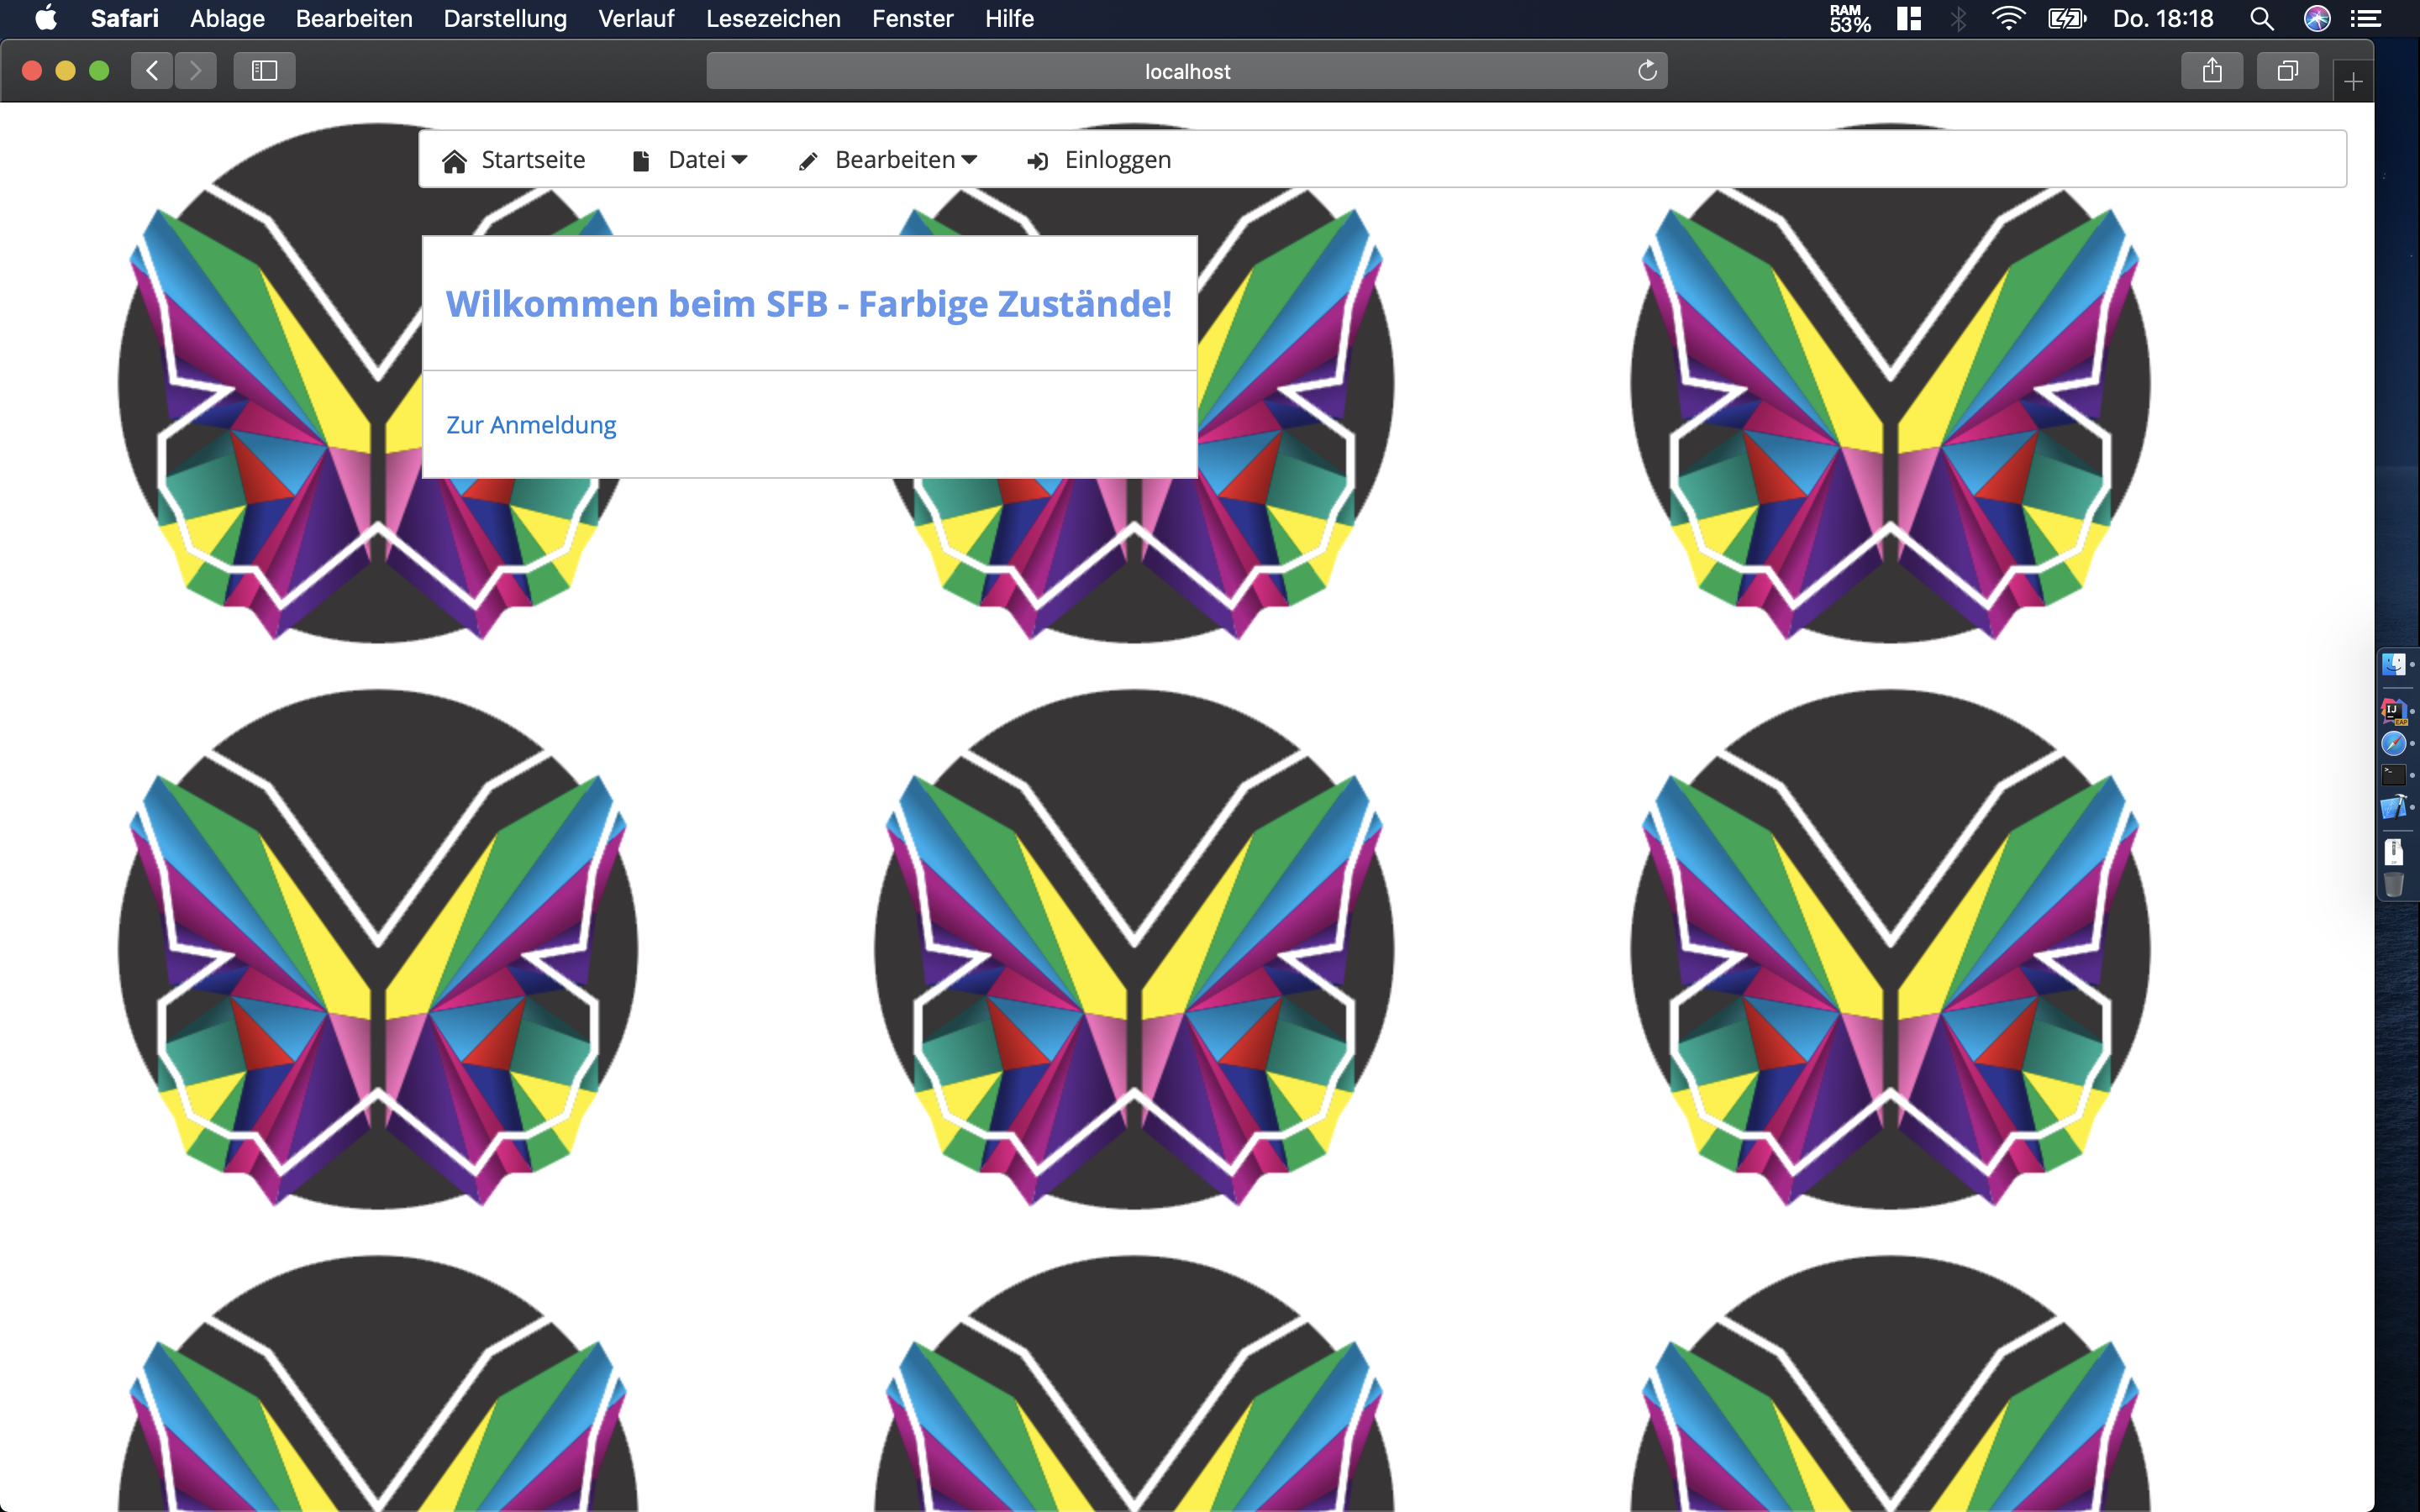
\includegraphics[width=1\textwidth]{Screenshots/311StartSite.png}
\textit{Abbildung 3.1.1.1: Startseite}
} \\

Hier kann man nun auf den Button \textit{Zur Anmeldung} drücken, um zur \hyperlink{sc3.1.1.2}{Loginseite} weitergeleitet zu werden. Ein valider Login ist der Benutzername \textit{admin} und das Passwort \textit{12345678}. \\

\hypertarget{sc3.1.1.2}{
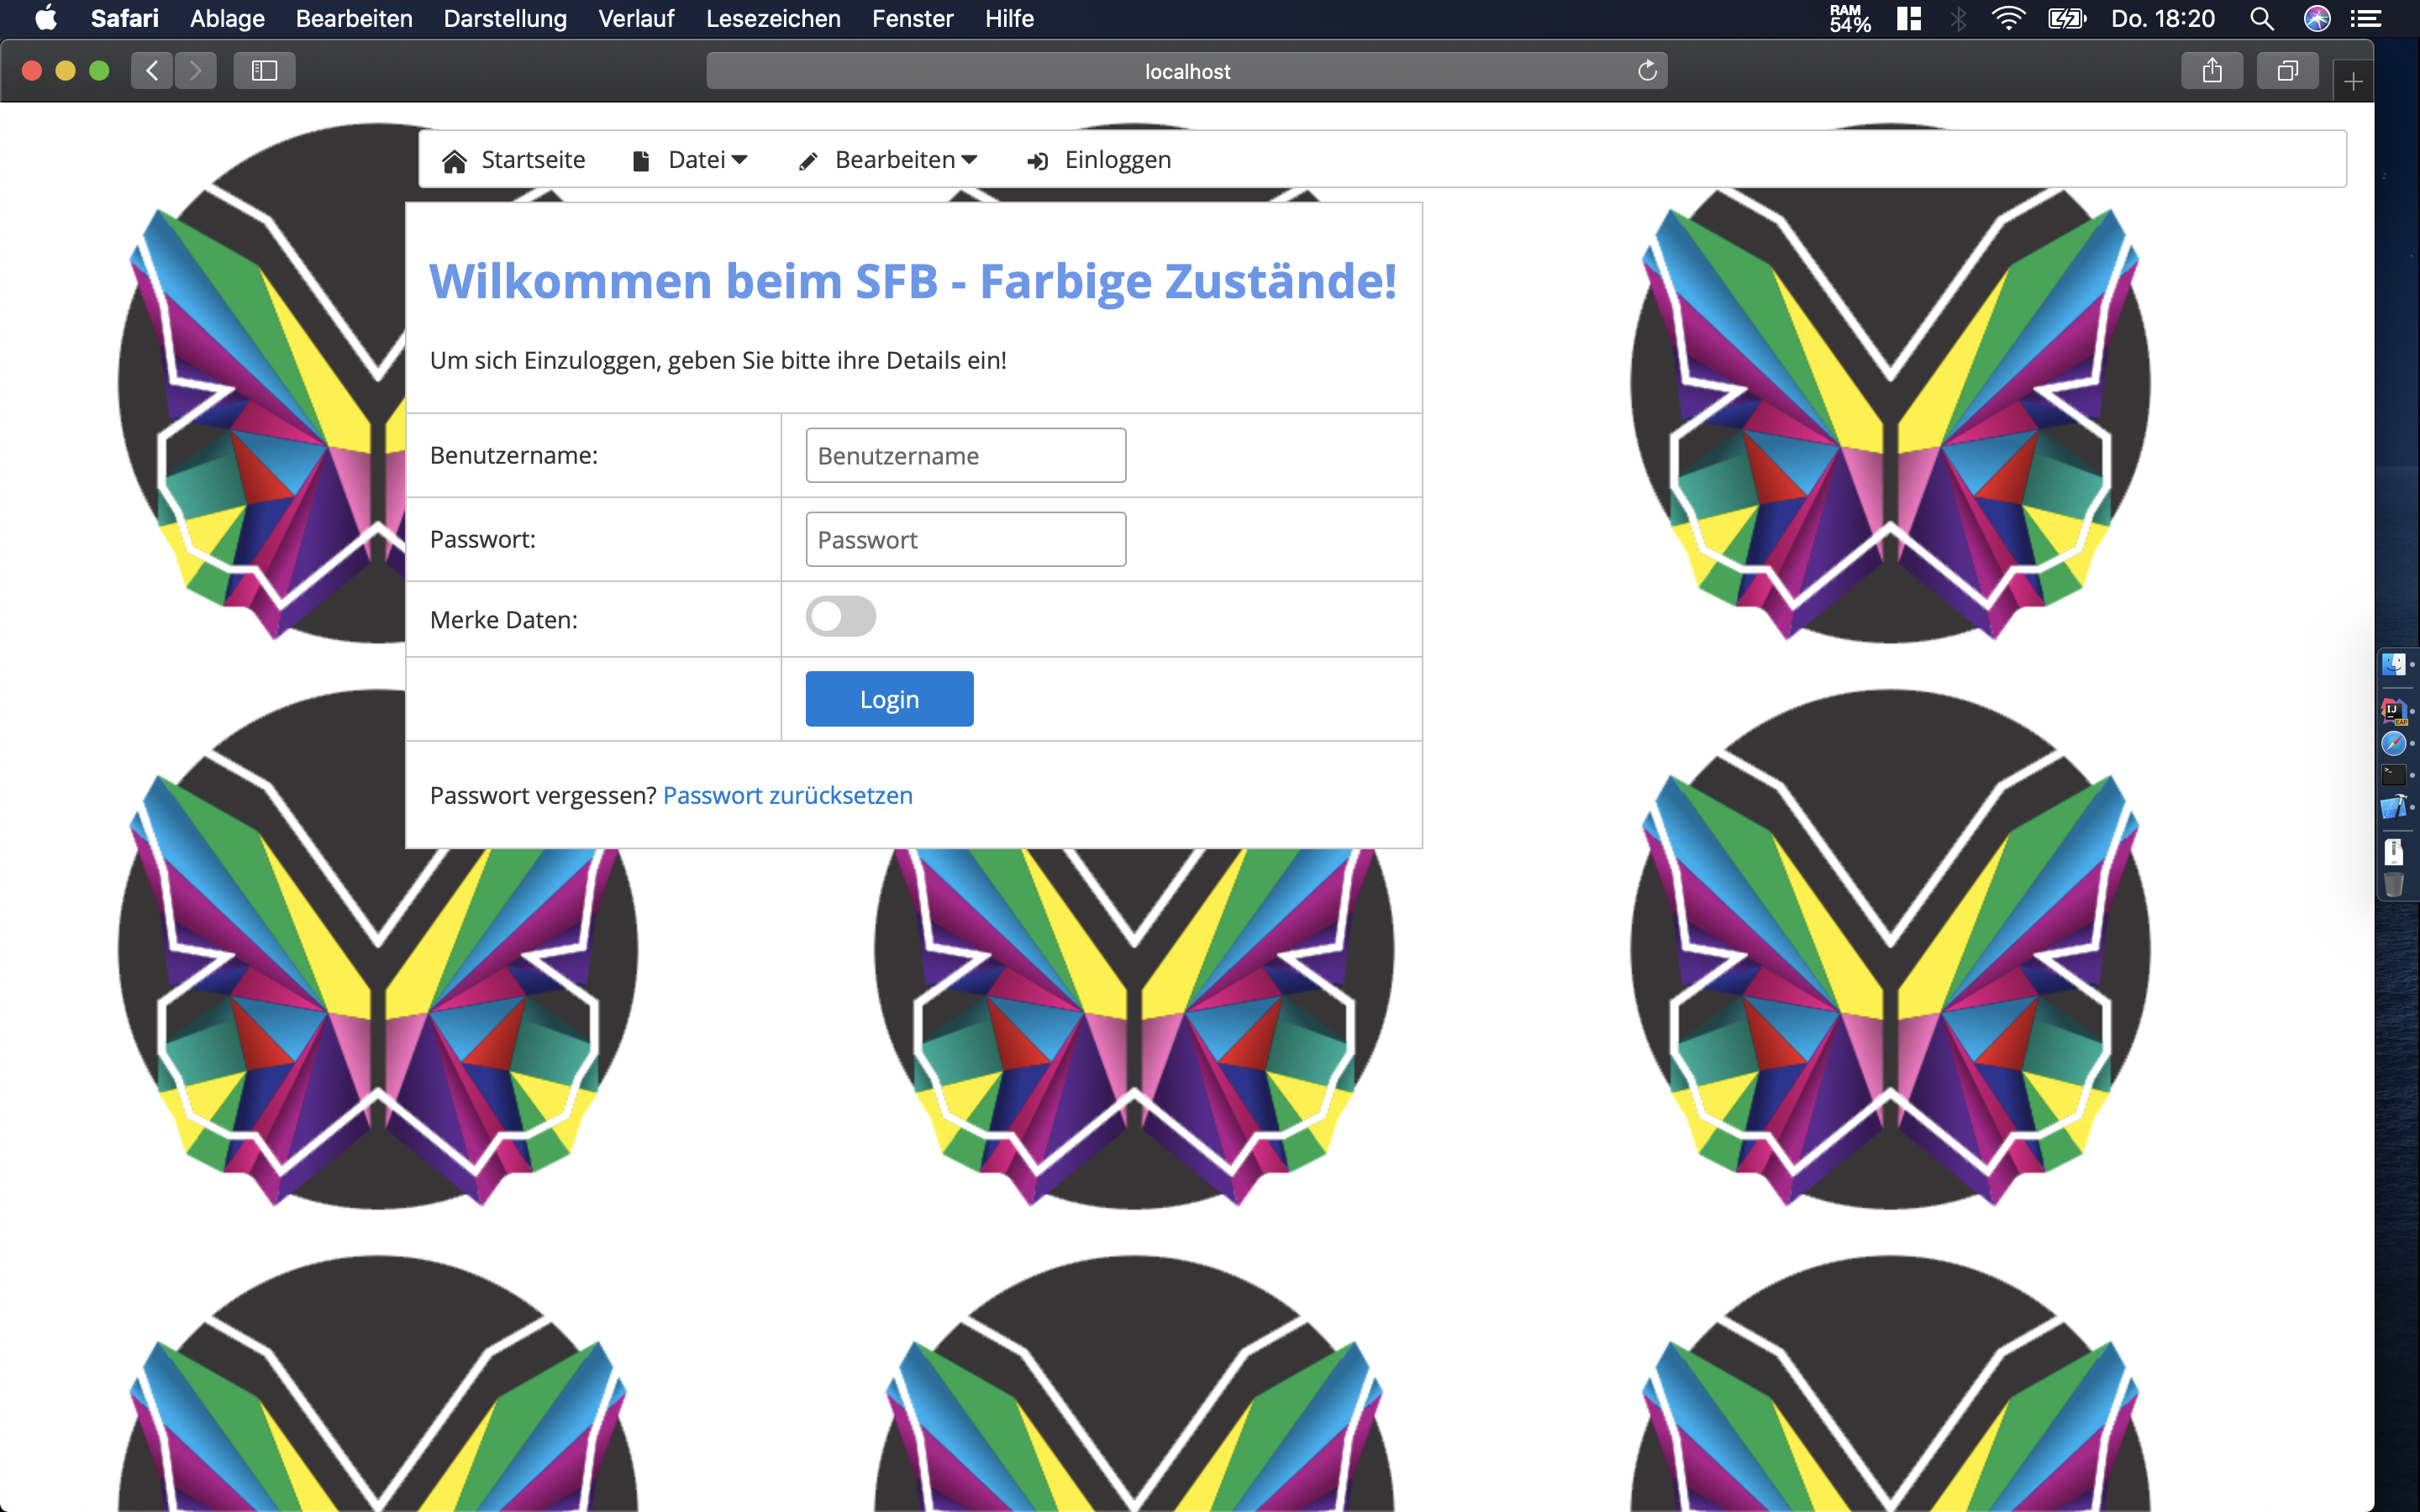
\includegraphics[width=1\textwidth]{Screenshots/311LoginSite.png}
\textit{Abbildung 3.1.1.2: Loginseite}
} \\

Jetzt haben wir uns als erstes mit einem falschen Passwort angemeldet, was eine Fehlermeldung wirft, wie man auf dem nächsten  \hyperlink{sc3.1.1.3}{Screenshot} in der oberen Ecke sieht.\\

\hypertarget{sc3.1.1.3}{
\includegraphics[width=1\textwidth]{Screenshots/311wrongPassword.png}
\textit{Abbildung 3.1.1.3: Falsches Passwort für Admin eingegeben}
} \\

Anschließend wurde versucht, sich mit den validen Logindaten des Admins einzuloggen und man kommt auf die \hyperlink{sc3.1.1.4}{Startseite des Admins}. \\

\hypertarget{sc3.1.1.4}{
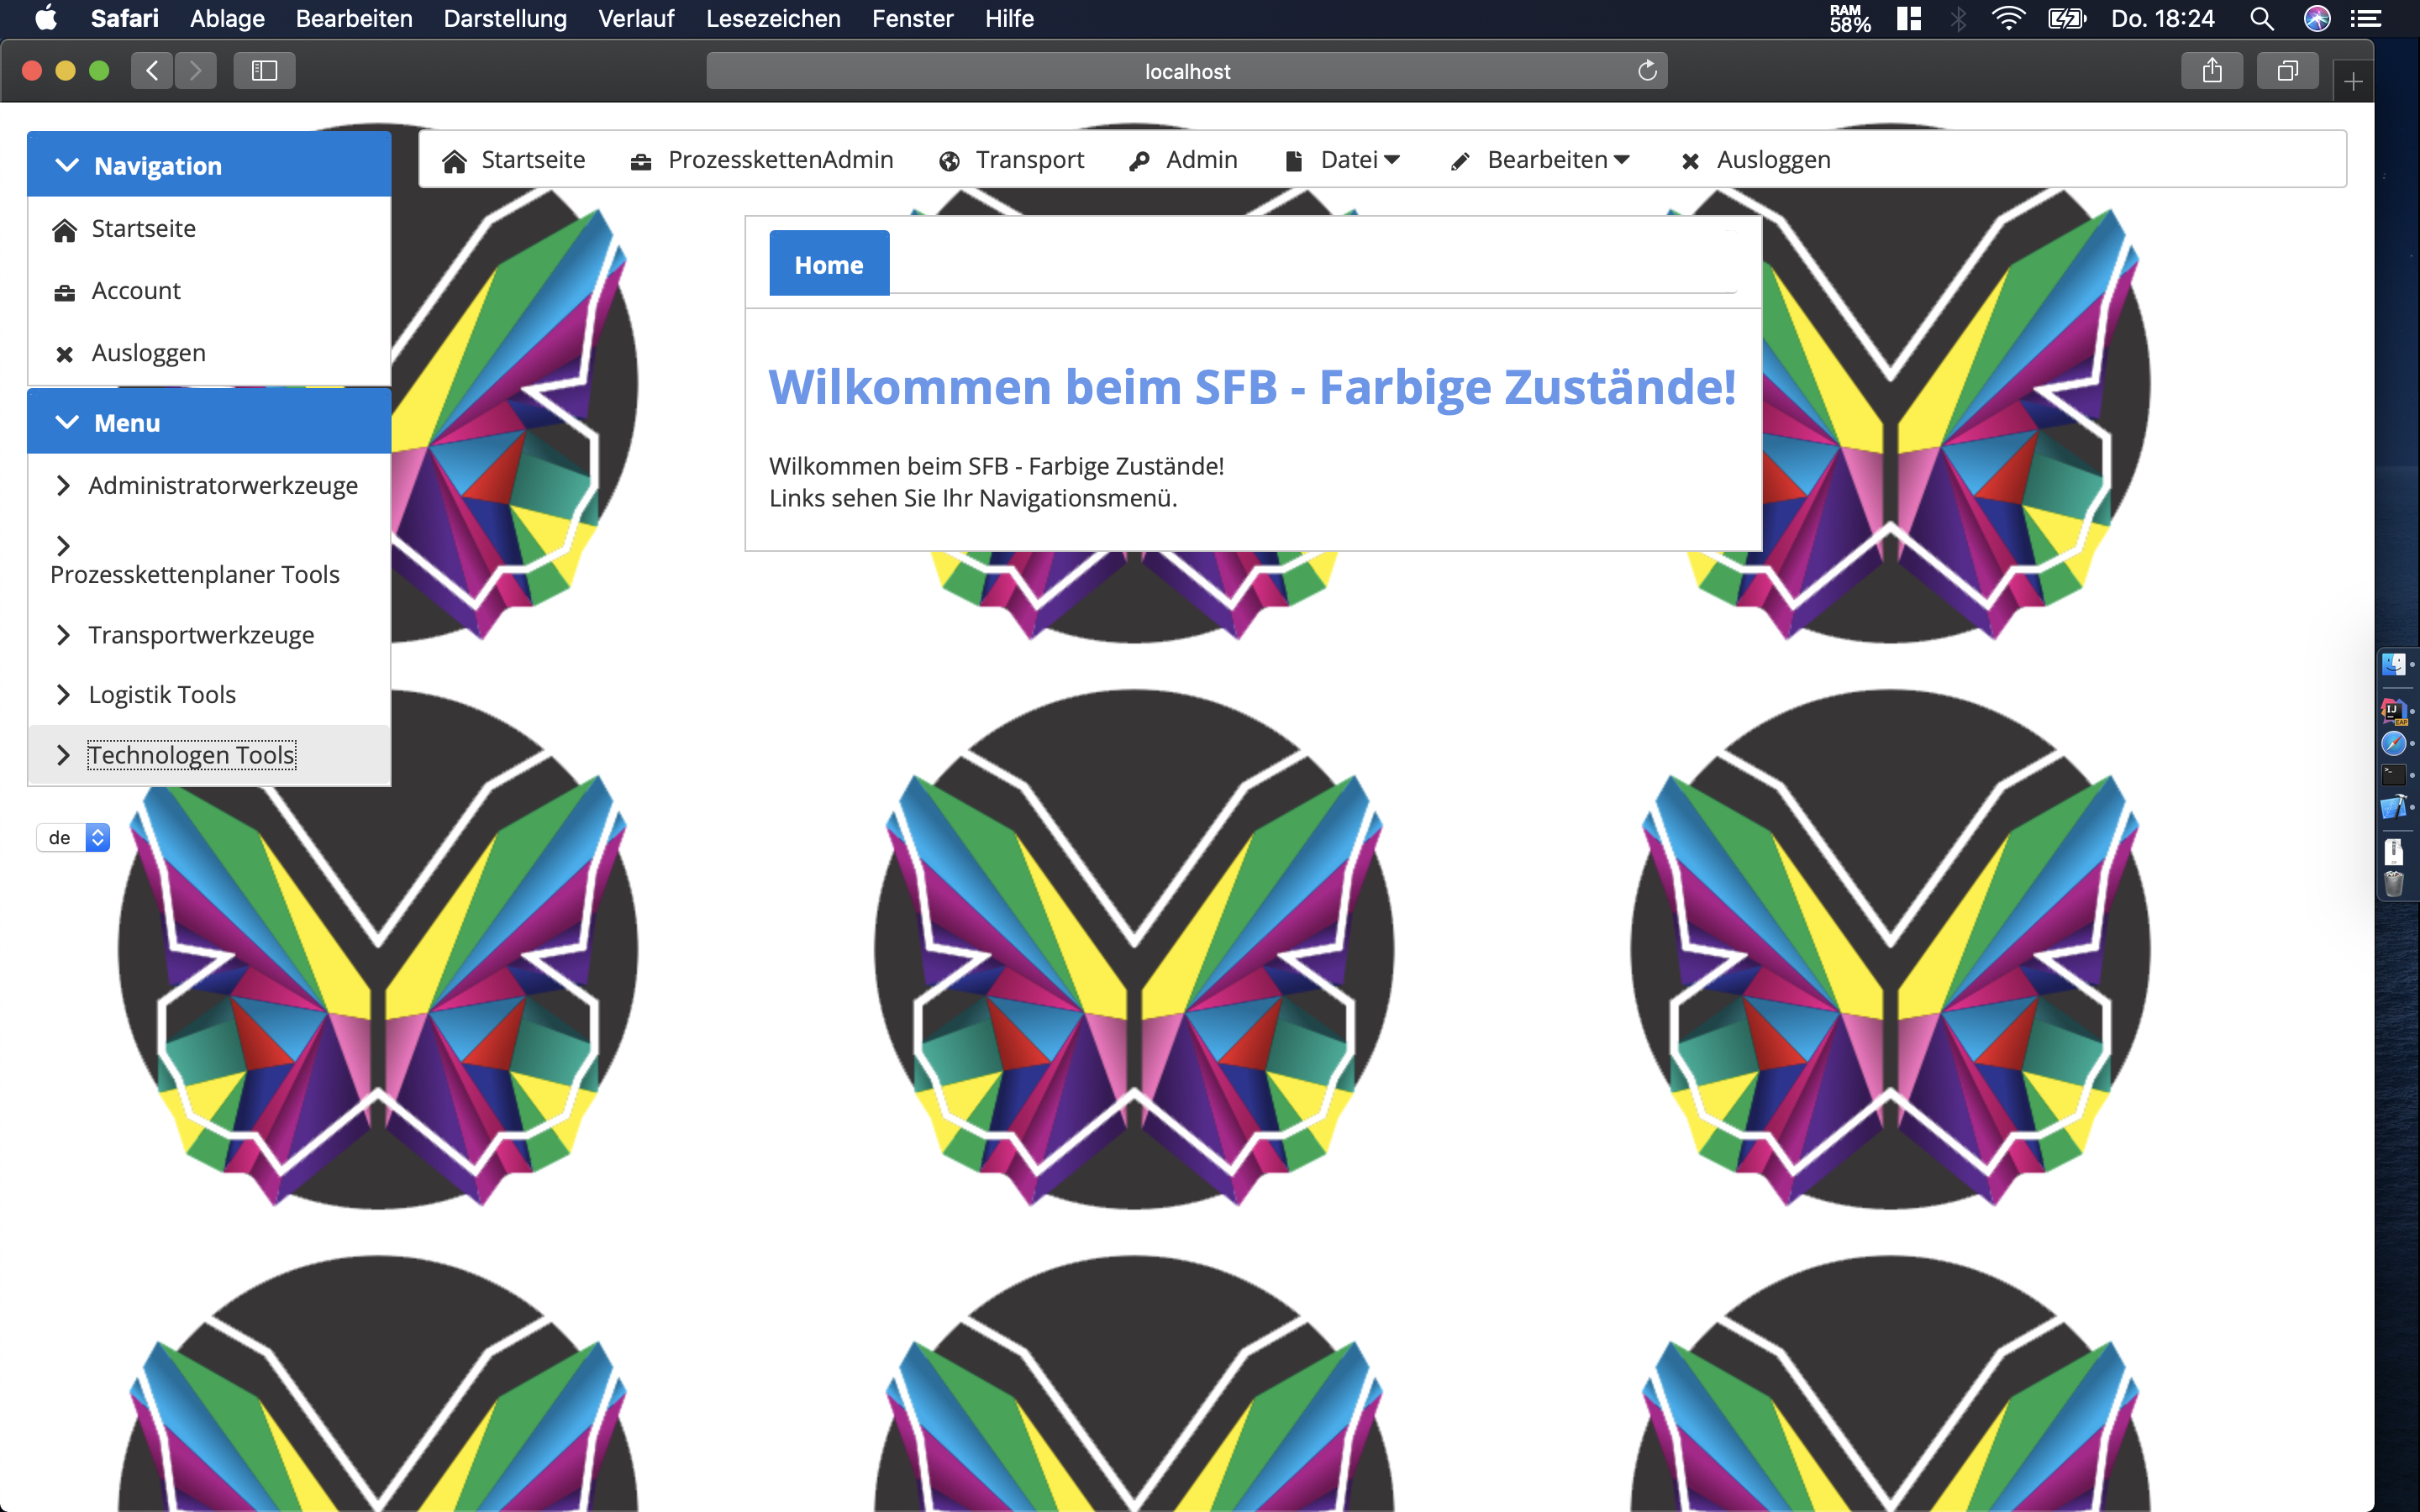
\includegraphics[width=1\textwidth]{Screenshots/311AdminView.png}
\textit{Abbildung 3.1.1.4: Richtiges Passwort für Admin eingegeben}
} \\

Jetzt wurde sich noch versucht, mit den validen Logindaten für den Technologen einzuloggen. Man wird auf die \hyperlink{sc3.1.1.5}{Startseite des Technologen} weitergeleitet. \\

\hypertarget{sc3.1.1.5}{
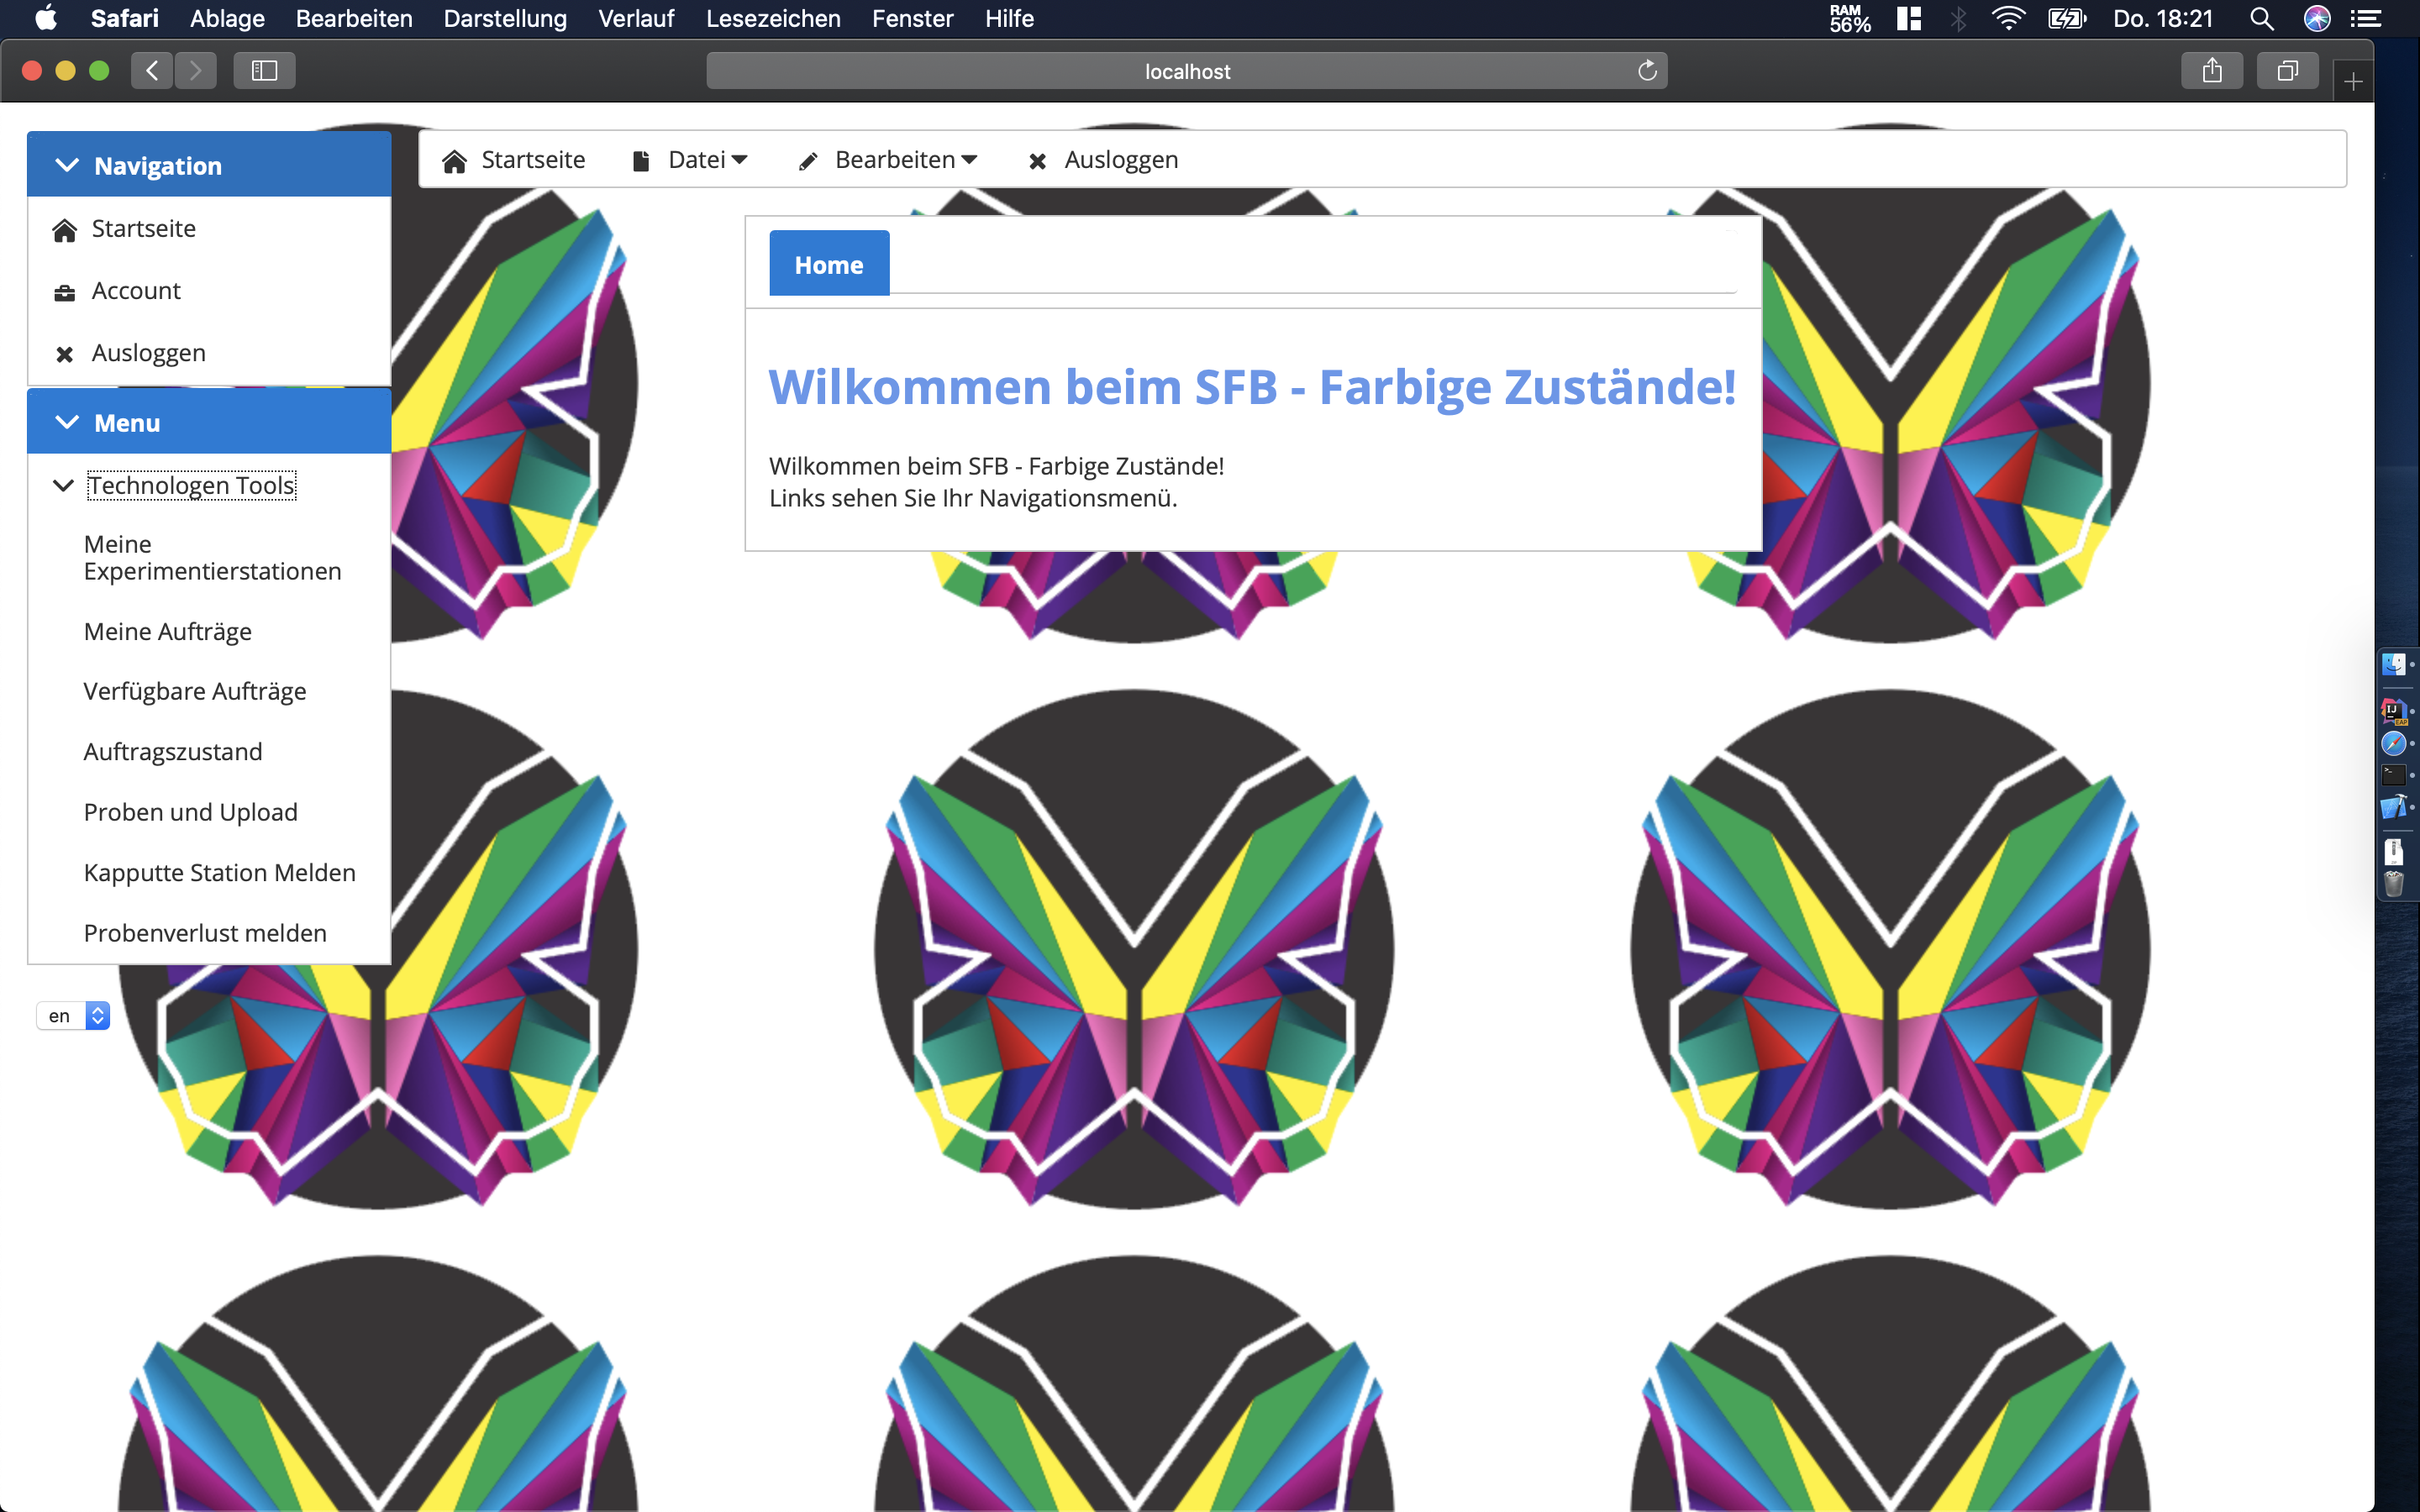
\includegraphics[width=1\textwidth]{Screenshots/311TechnologeView.png}
\textit{Abbildung 3.1.1.5: Richtiges Passwort für Technologen eingegeben}
} \\

Wie man in den Beispielen sehen kann, kann man sich mit unterschiedlichen Benutzern einloggen, welche unterschiedliche den Rollen entsprechende Features haben. Man muss das richtige Passwort für den Benutzernamen eingeben, um sich einloggen zu können. Die Tests verliefen erfolgreich. \\ 

\hypertarget{sc3.1.1.6}{
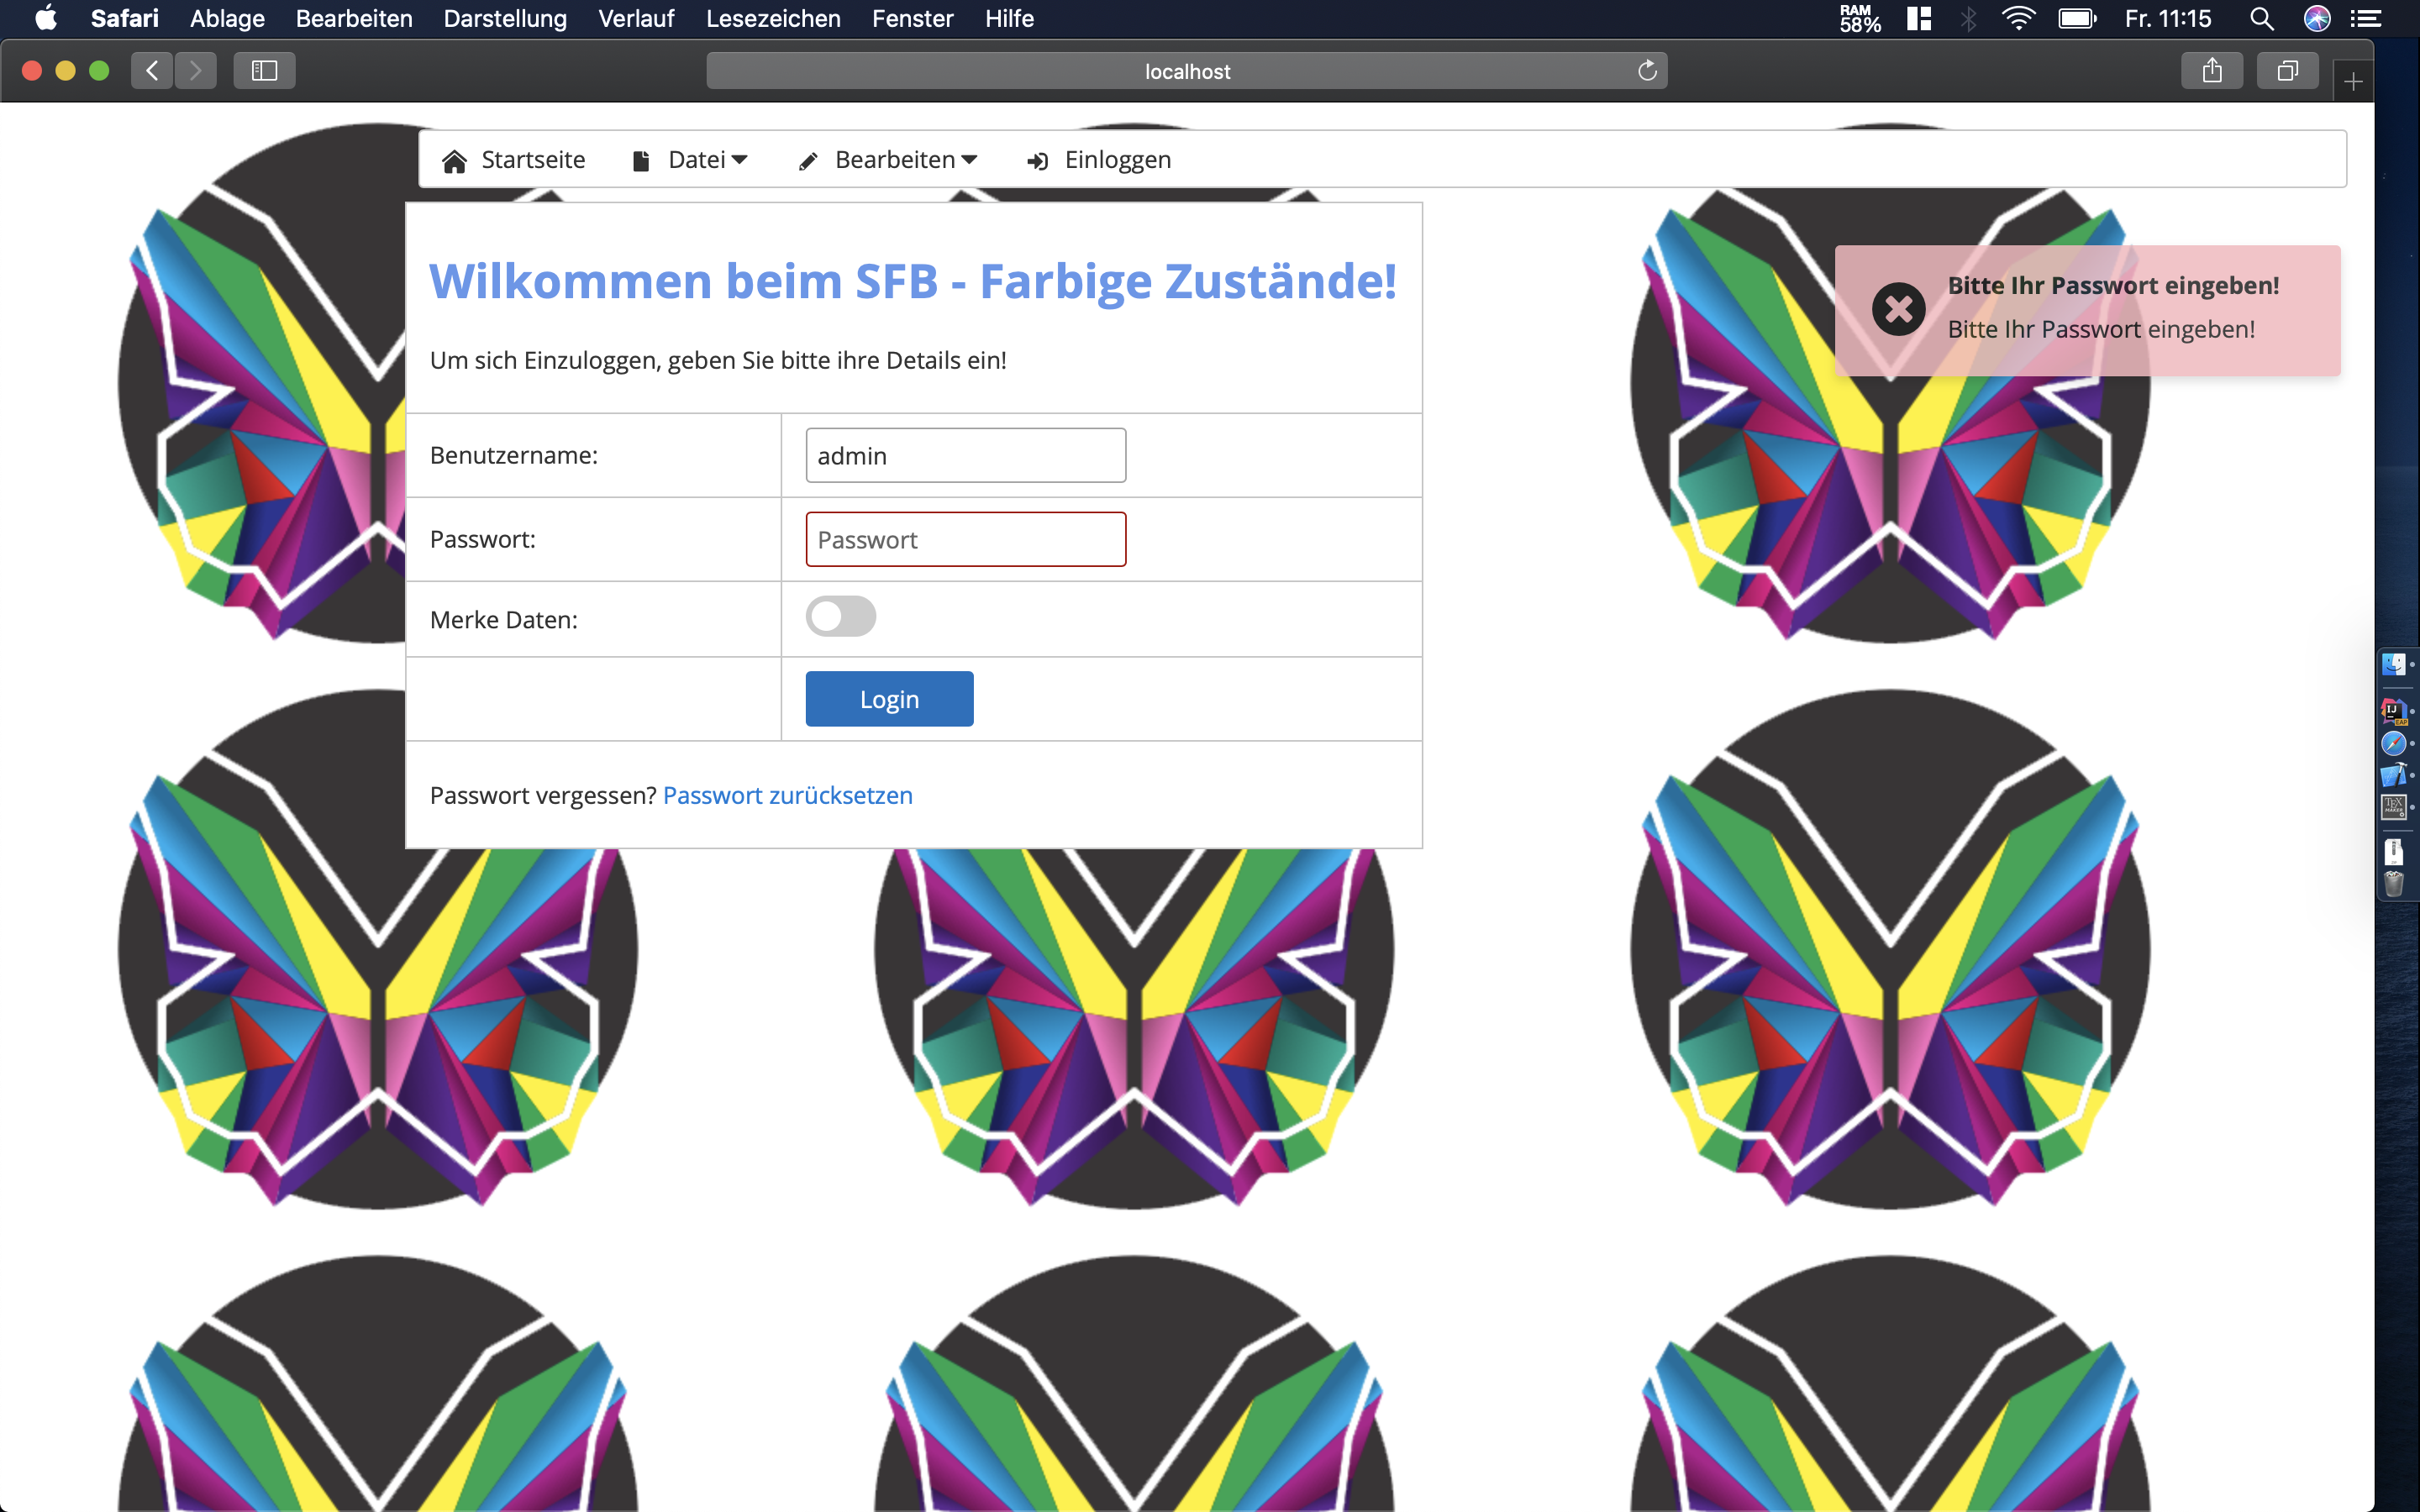
\includegraphics[width=1\textwidth]{Screenshots/311BittePasswordEingeben.png}\\ \textit{Abbildung 3.1.1.6: Benutzer ohne password}
} \\

\hypertarget{sc3.1.1.7}{
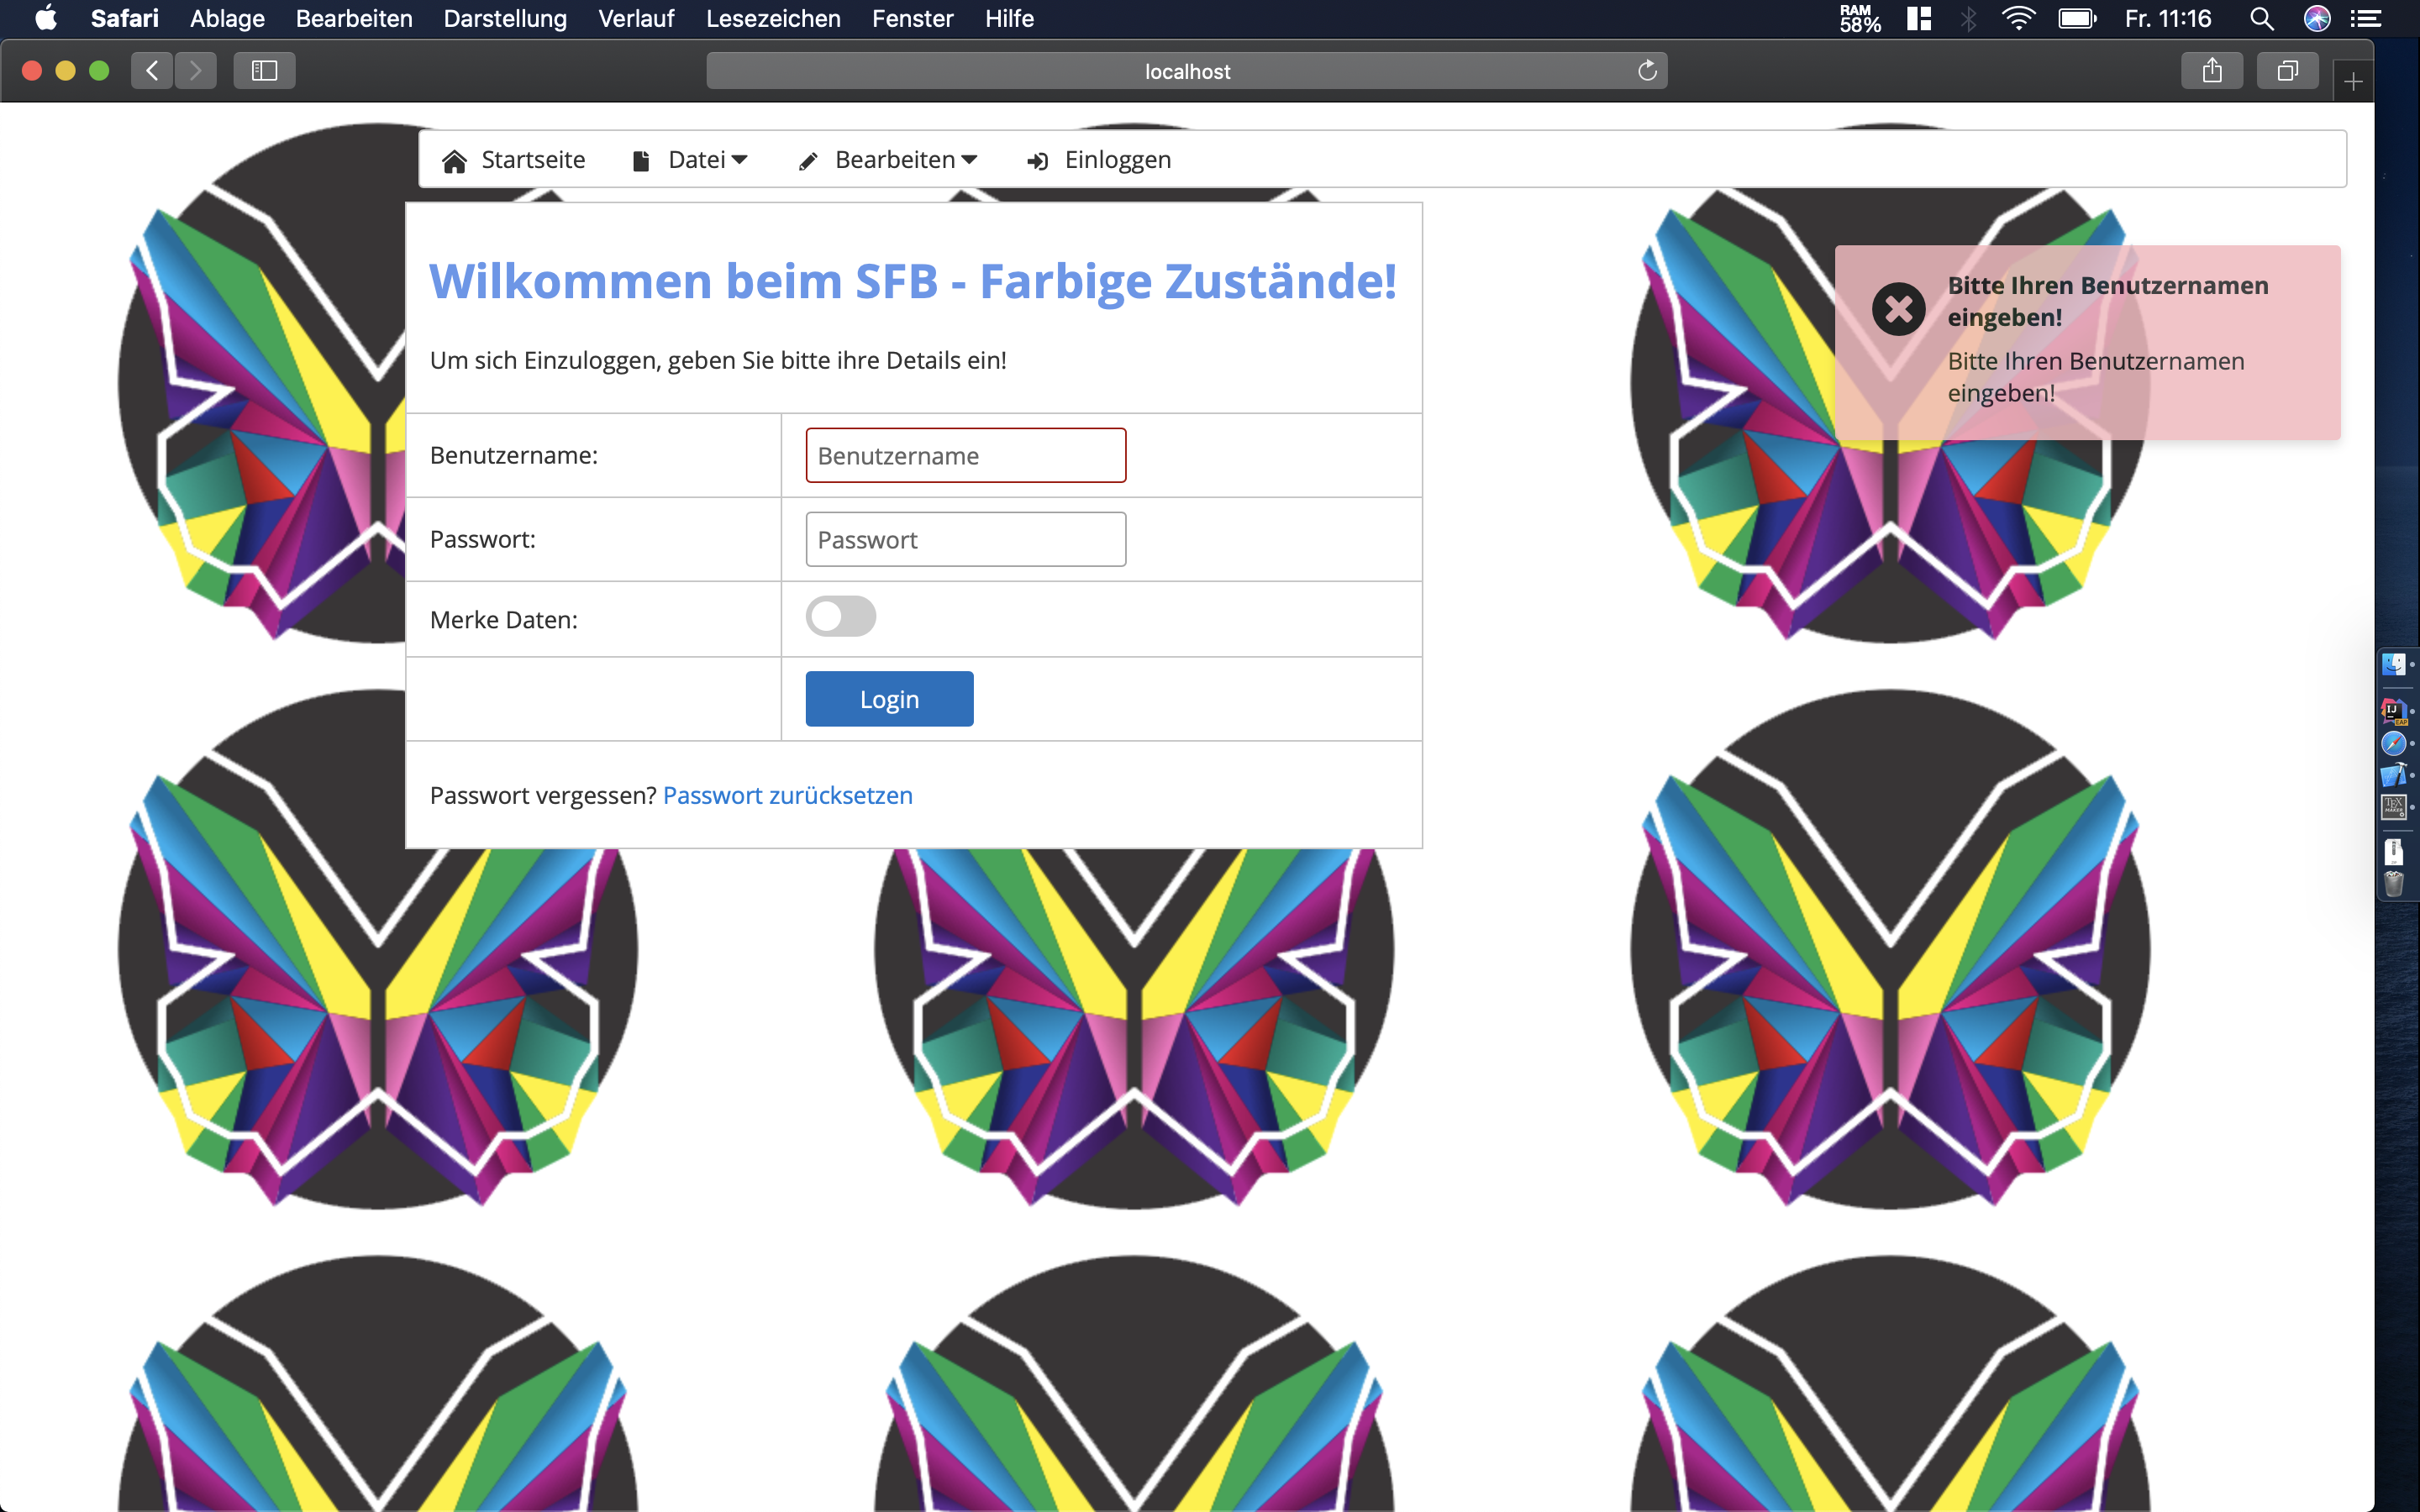
\includegraphics[width=1\textwidth]{Screenshots/311PasswordohneBenutzer.png}
\textit{Abbildung 3.1.1.7: password ohne Benutzer}
} \\
%%%Create User
%%Formular
Für die Erstellung und Kontrolle der Benutzer verfügt der Administrator über eine Tabelle und ein Formular.

Nun haben wir noch getestet, was passiert, wenn kein Benutzername eingegeben wird. Wie man sieht, wird eine  \hyperlink{sc3.1.1.8}{Fehlermeldung} ausgegeben. \\

\hypertarget{sc3.1.1.8}{
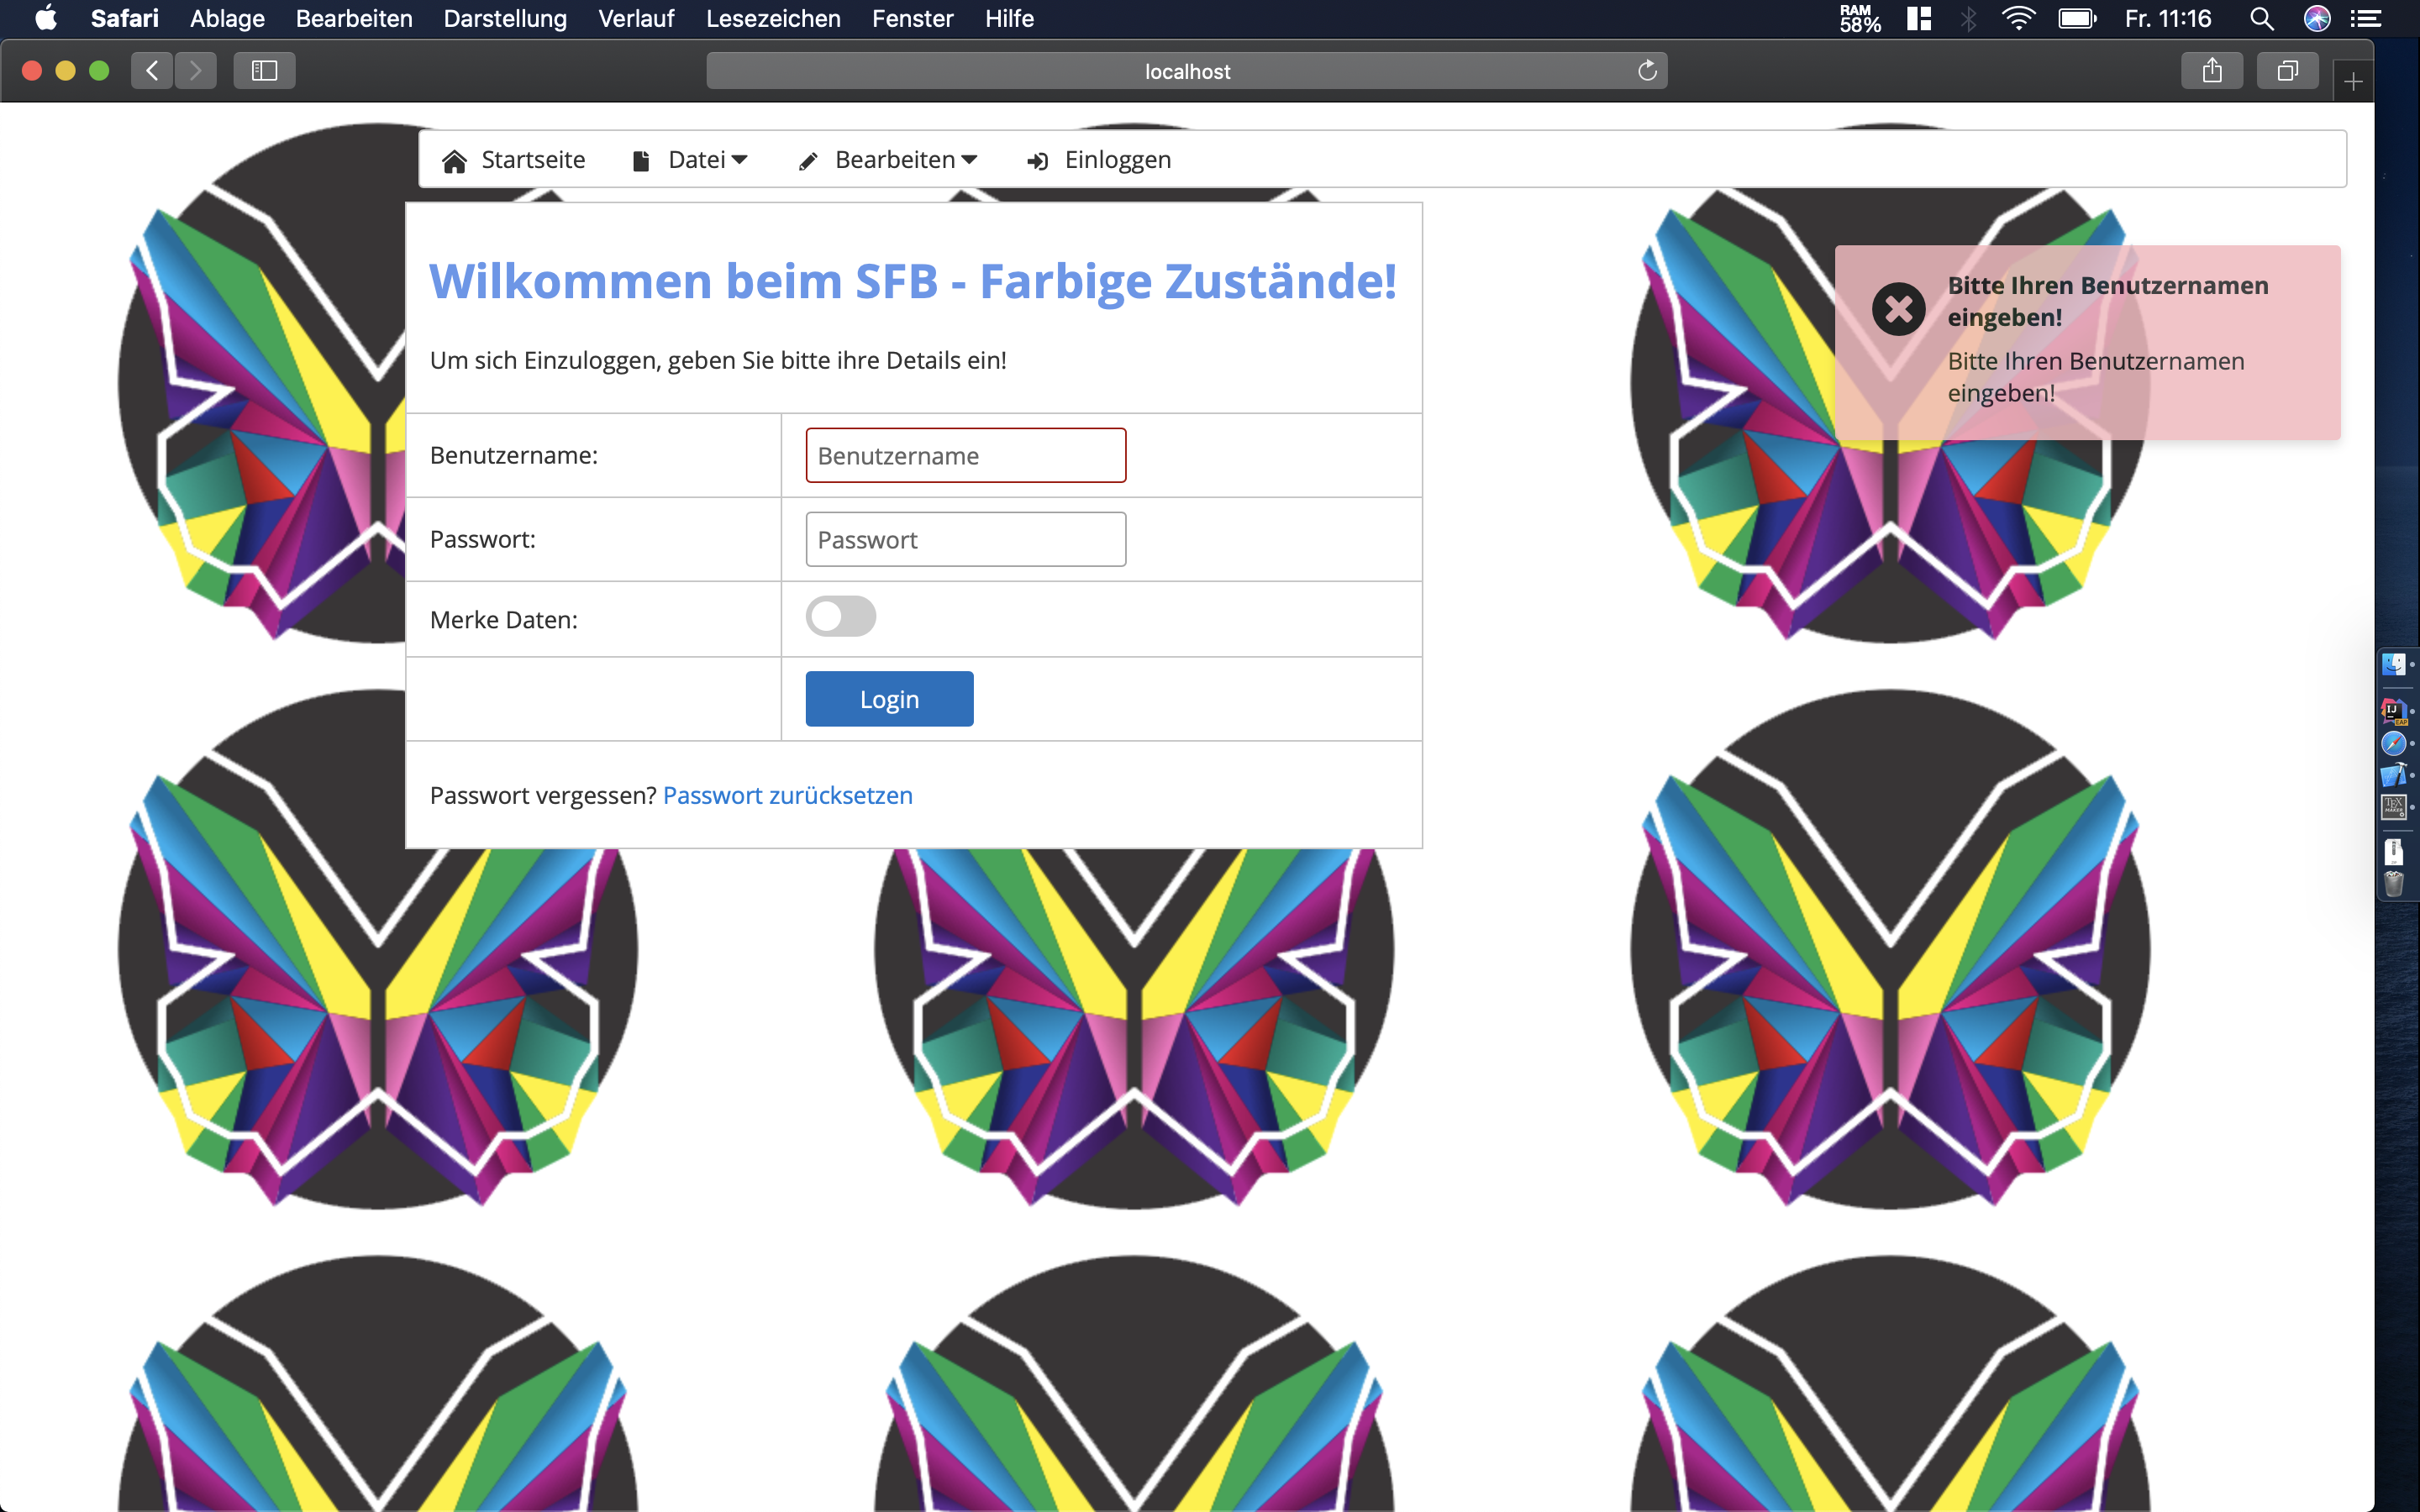
\includegraphics[width=1\textwidth]{Screenshots/311PasswordohneBenutzer.png}
\textit{Abbildung 3.1.1.8: Fehlermeldung: Bitte Ihren Benutzernamen eingeben!}
} \\

Zuletzt wurde getestet, was passiert, wenn kein Passwort eingegeben wurde. Es erscheint eine \hyperlink{sc3.1.1.9}{Fehlermeldung}, dass man das Passwort eingeben soll. 

\hypertarget{sc3.1.1.9}{
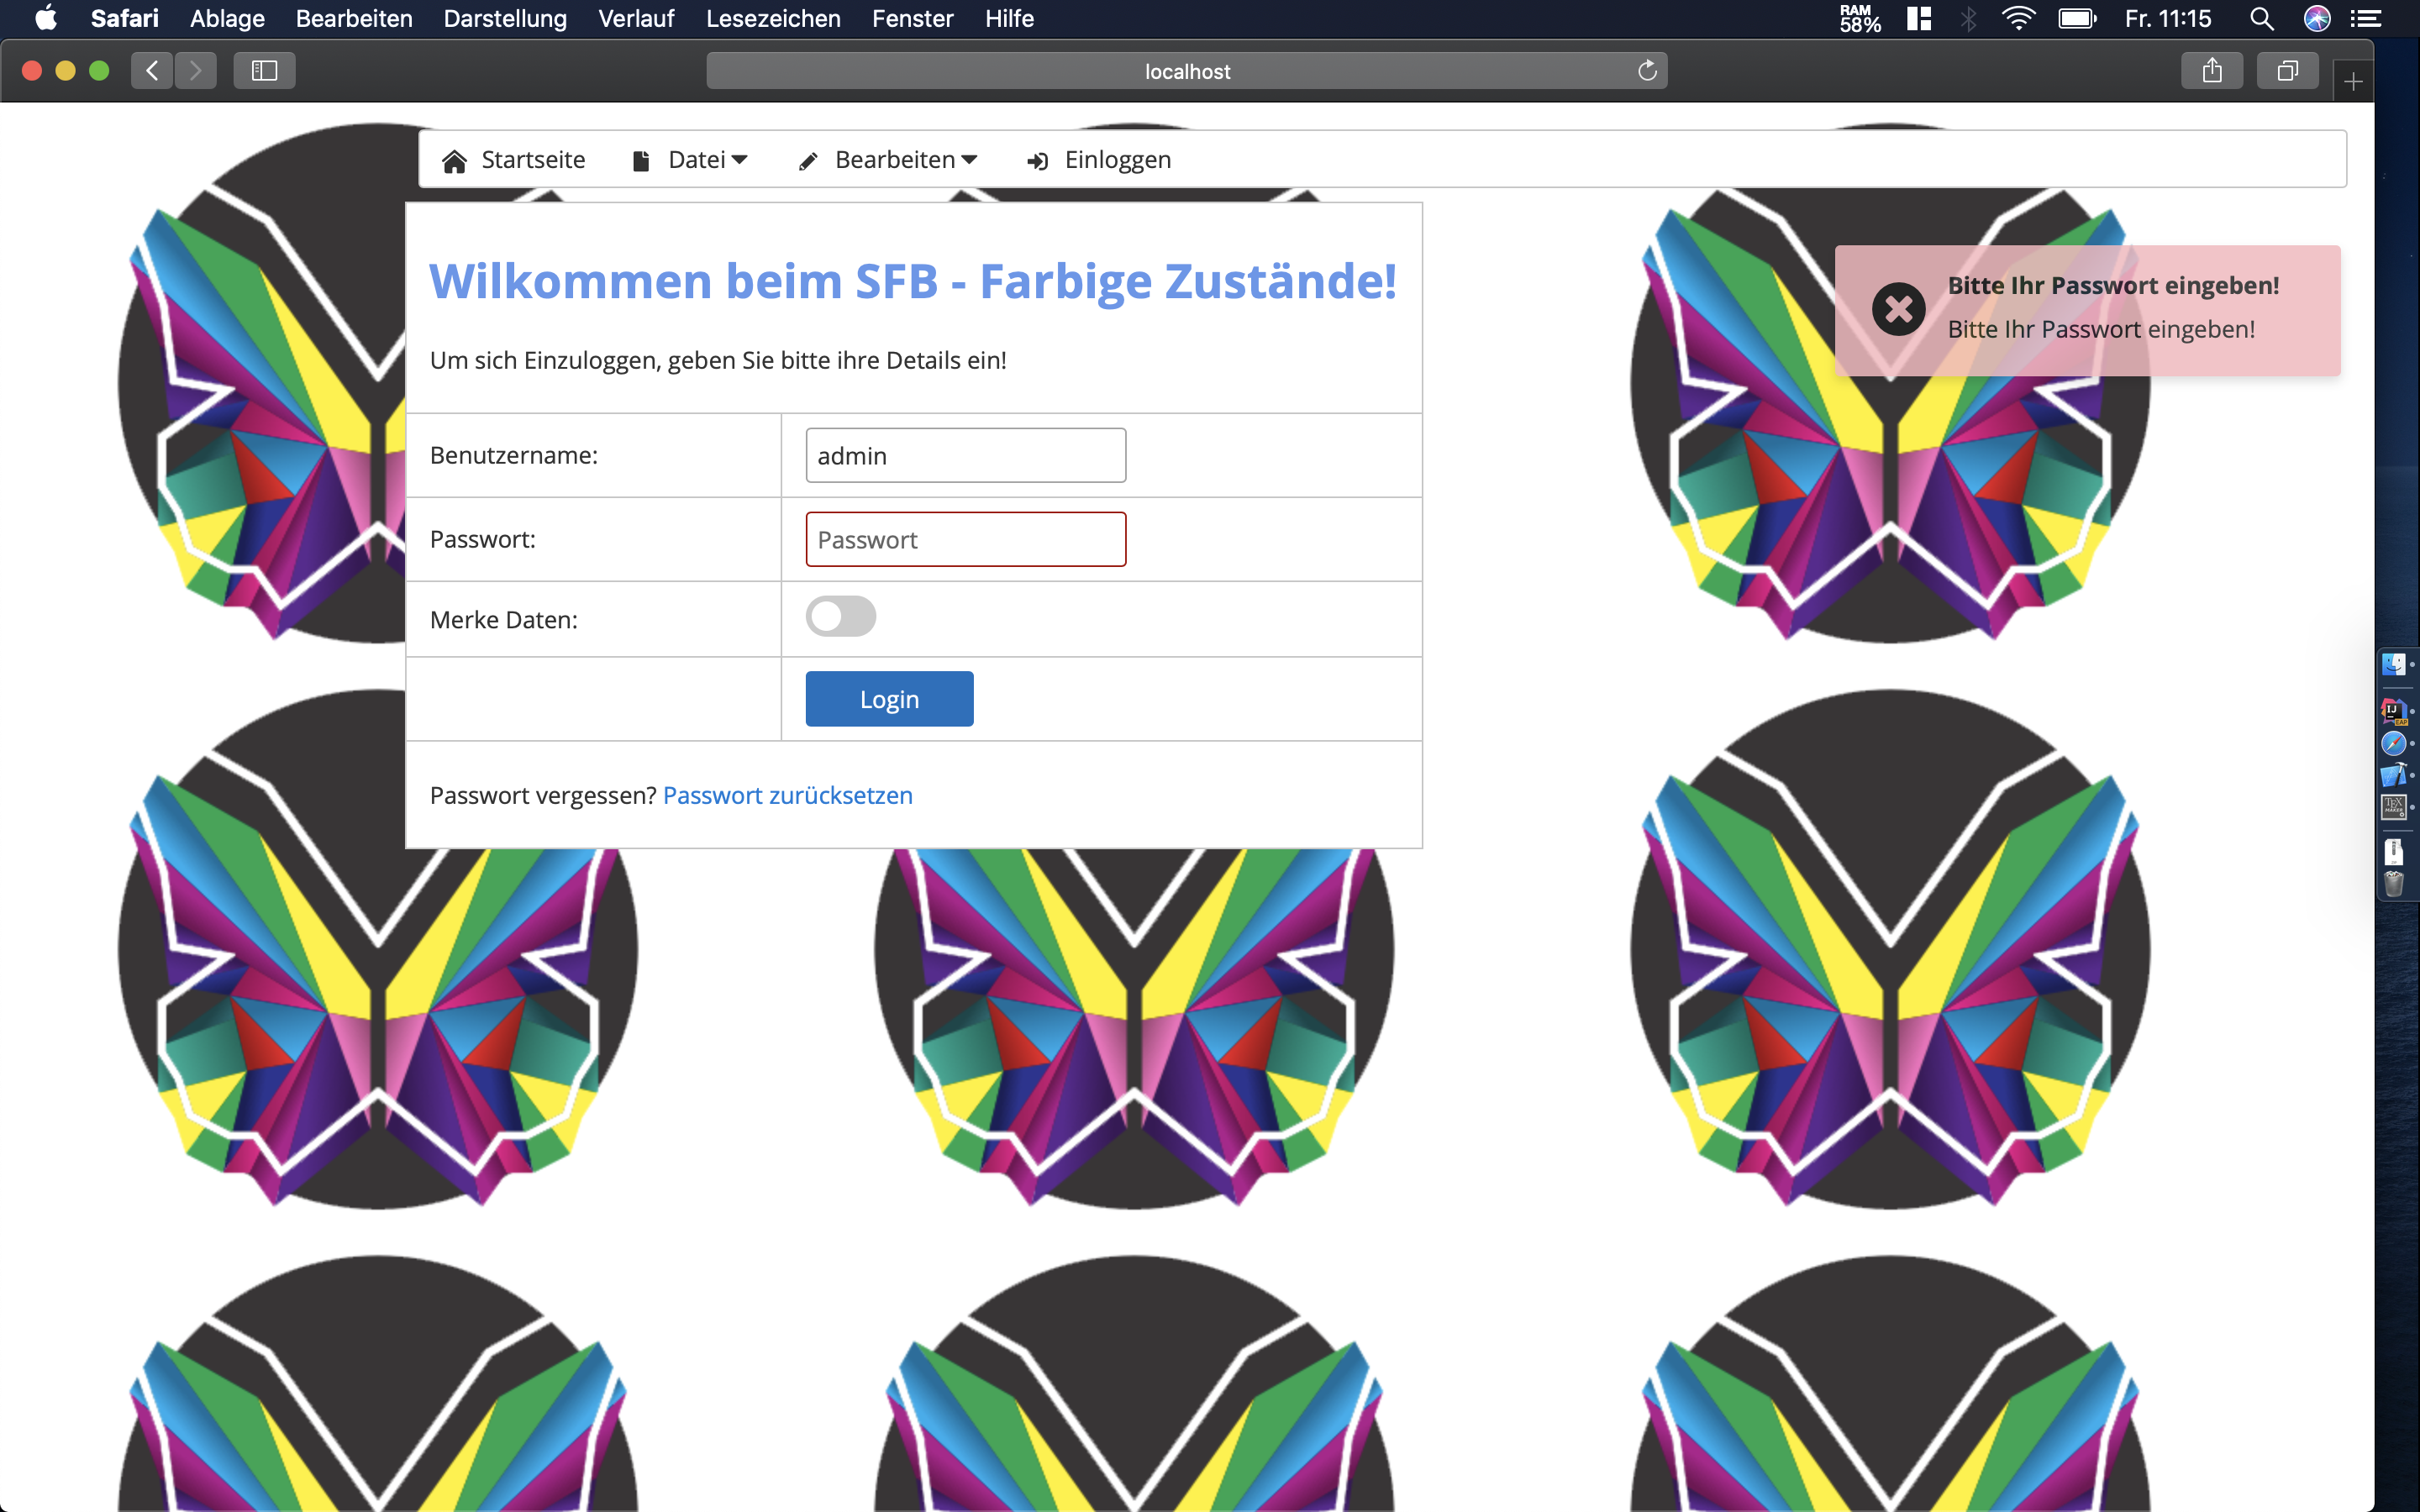
\includegraphics[width=1\textwidth]{Screenshots/311BittePasswordEingeben.png}
\textit{Abbildung 3.1.1.9: Fehlermeldung: Bitte Ihr Passwort eingeben!}
} \\

Wie man in den Beispielen sehen kann, kann man sich mit unterschiedlichen Benutzern einloggen, welche unterschiedliche den Rollen entsprechende Features haben. Man muss das richtige Passwort für den Benutzernamen eingeben, um sich einloggen zu können. Die Tests verliefen erfolgreich. \\ 

%%

\subsubsection{Anwendungsfall: Beispiel 2}
Für die Erstellung und Kontrolle der Benutzer verfügt der Administrator über eine Tabelle und ein Formular.

Um einen neuen Benutzer zu erstellen, muss der Administrator die erforderlichen Felder in das Formular eingeben. Der Administrator muss versuchen, die Daten ordnungsgemäß einzugeben, damit die Erstellung erfolgreich ist.

\hypertarget{sc3.1.2.1}{
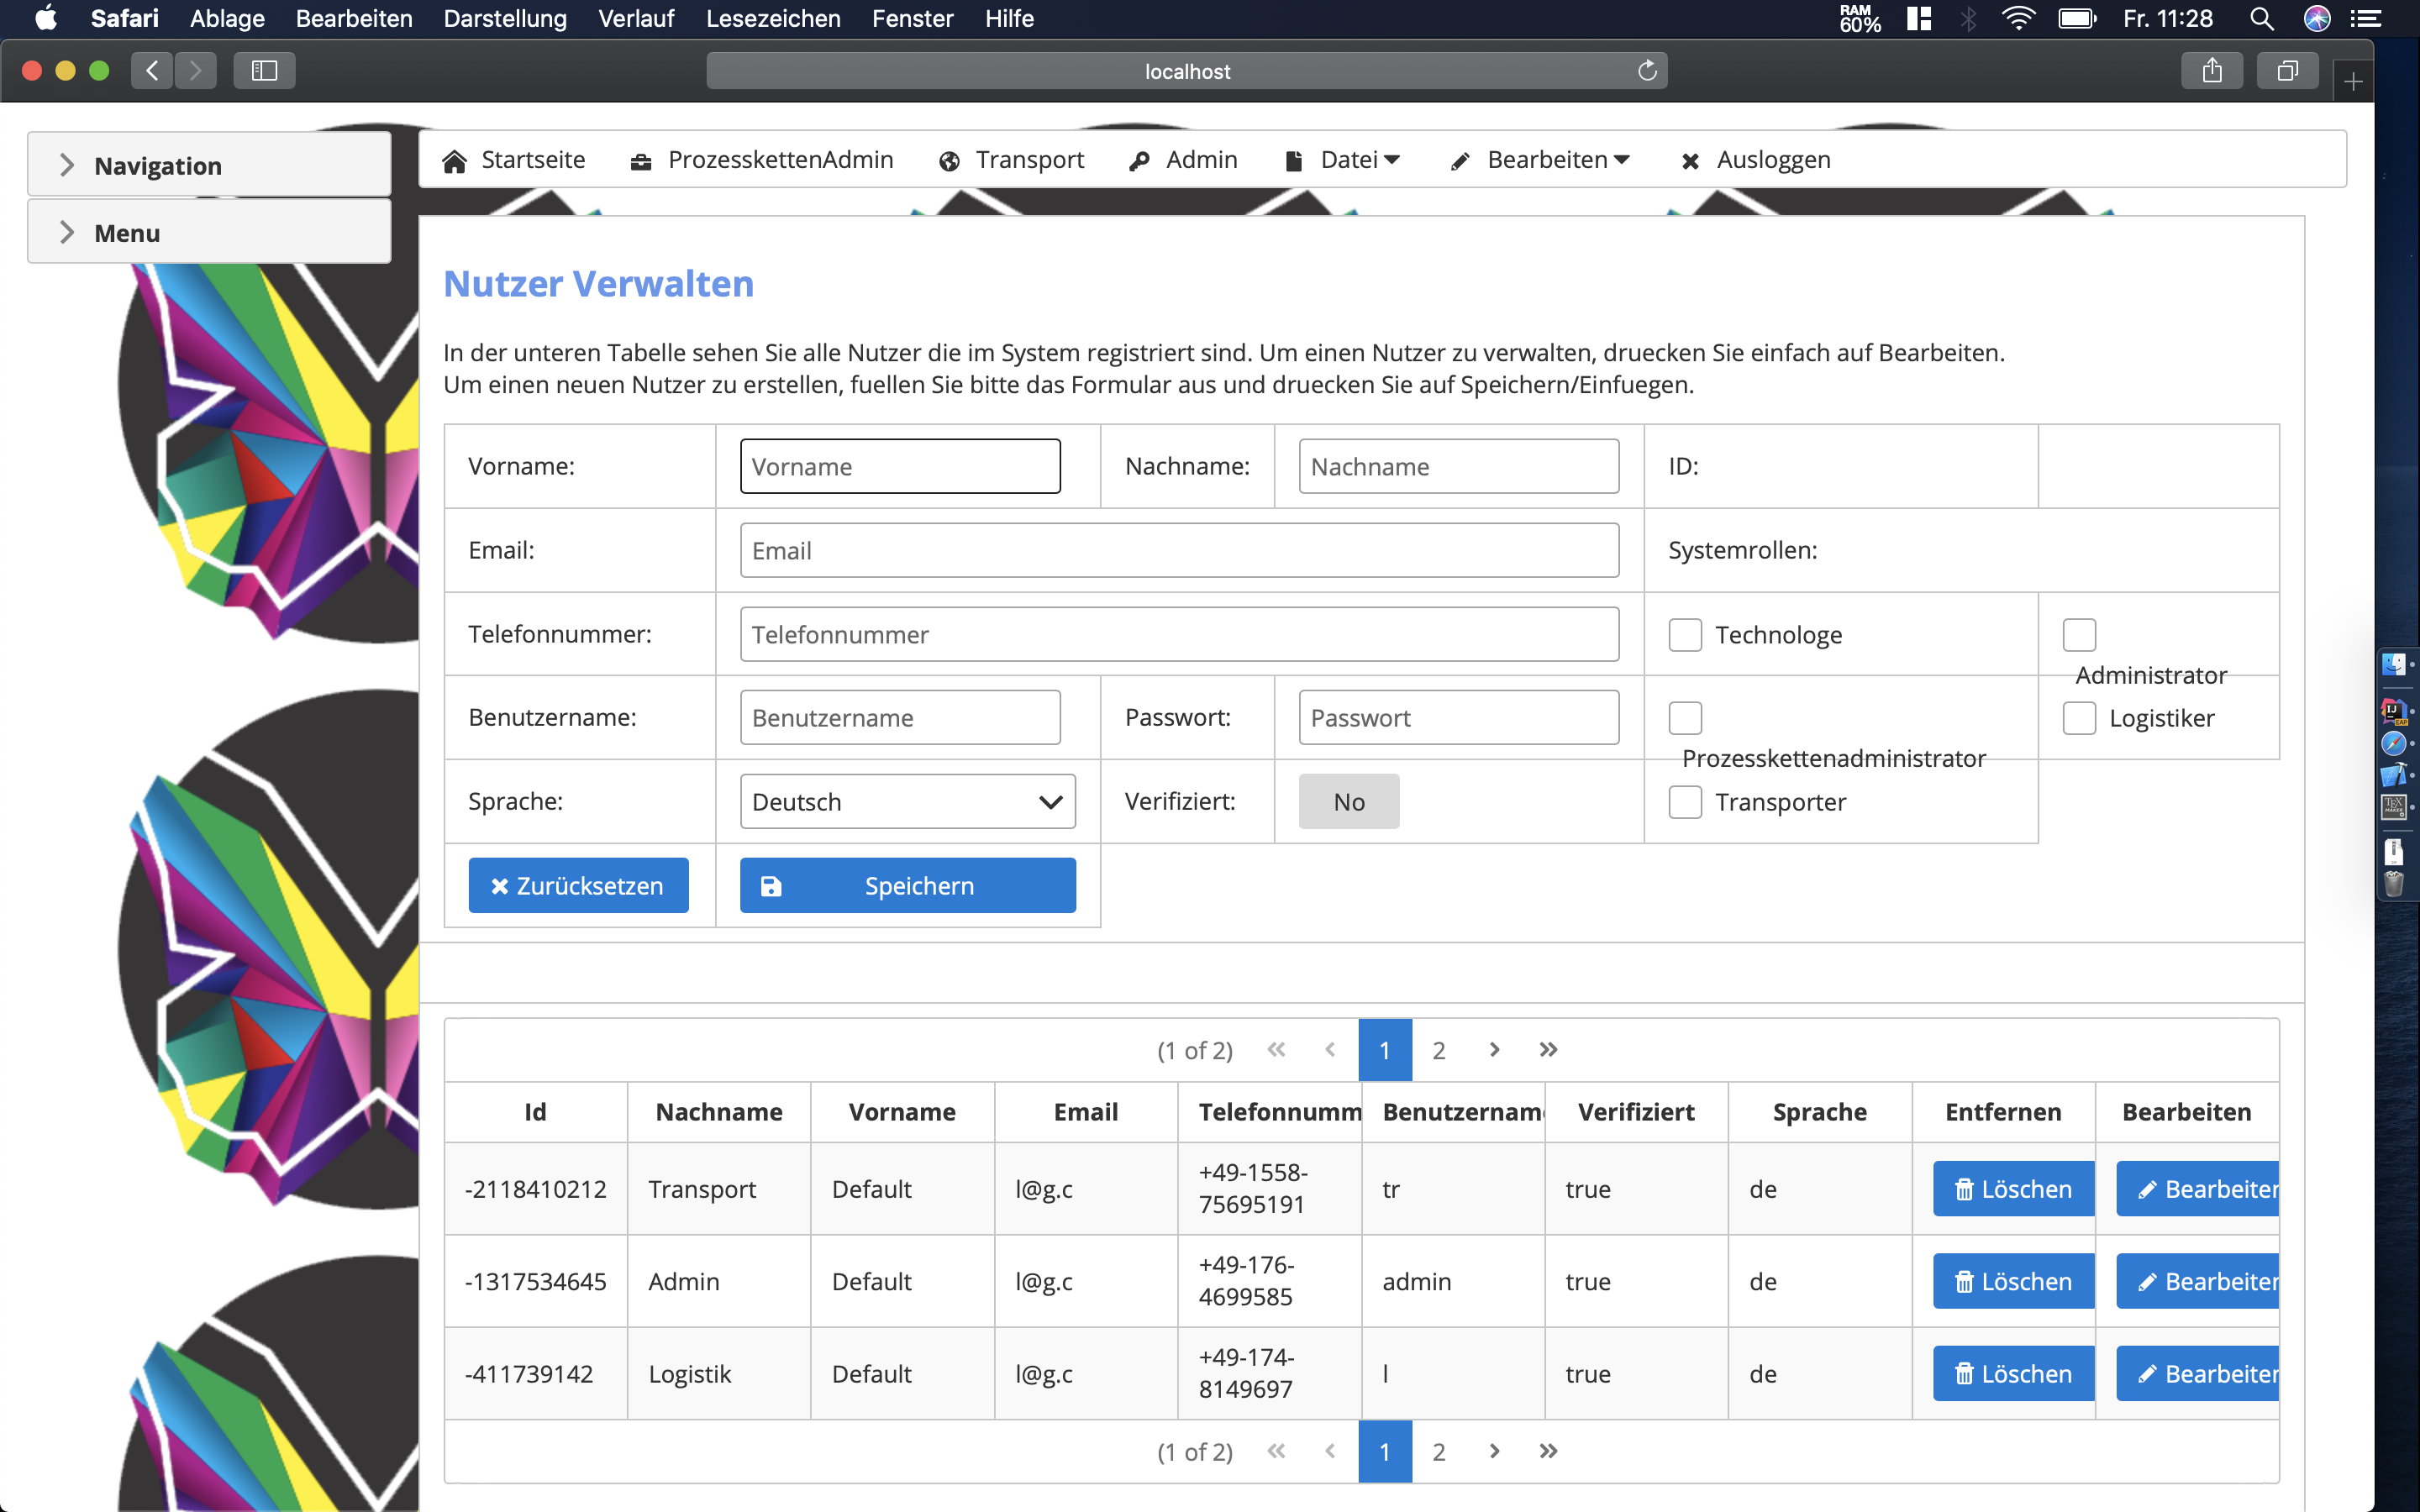
\includegraphics[width=1\textwidth]{Screenshots/UserErzeugenFormular.png}
\textit{Abbildung 3.1.1.8: Benutzer Formular and Tabelle von Benutzer}
} \\

In der folgenden Grafik erstellen wir einen Benutzer mit den entsprechenden Daten.
%%InitialData
\hypertarget{sc3.1.2.2}{
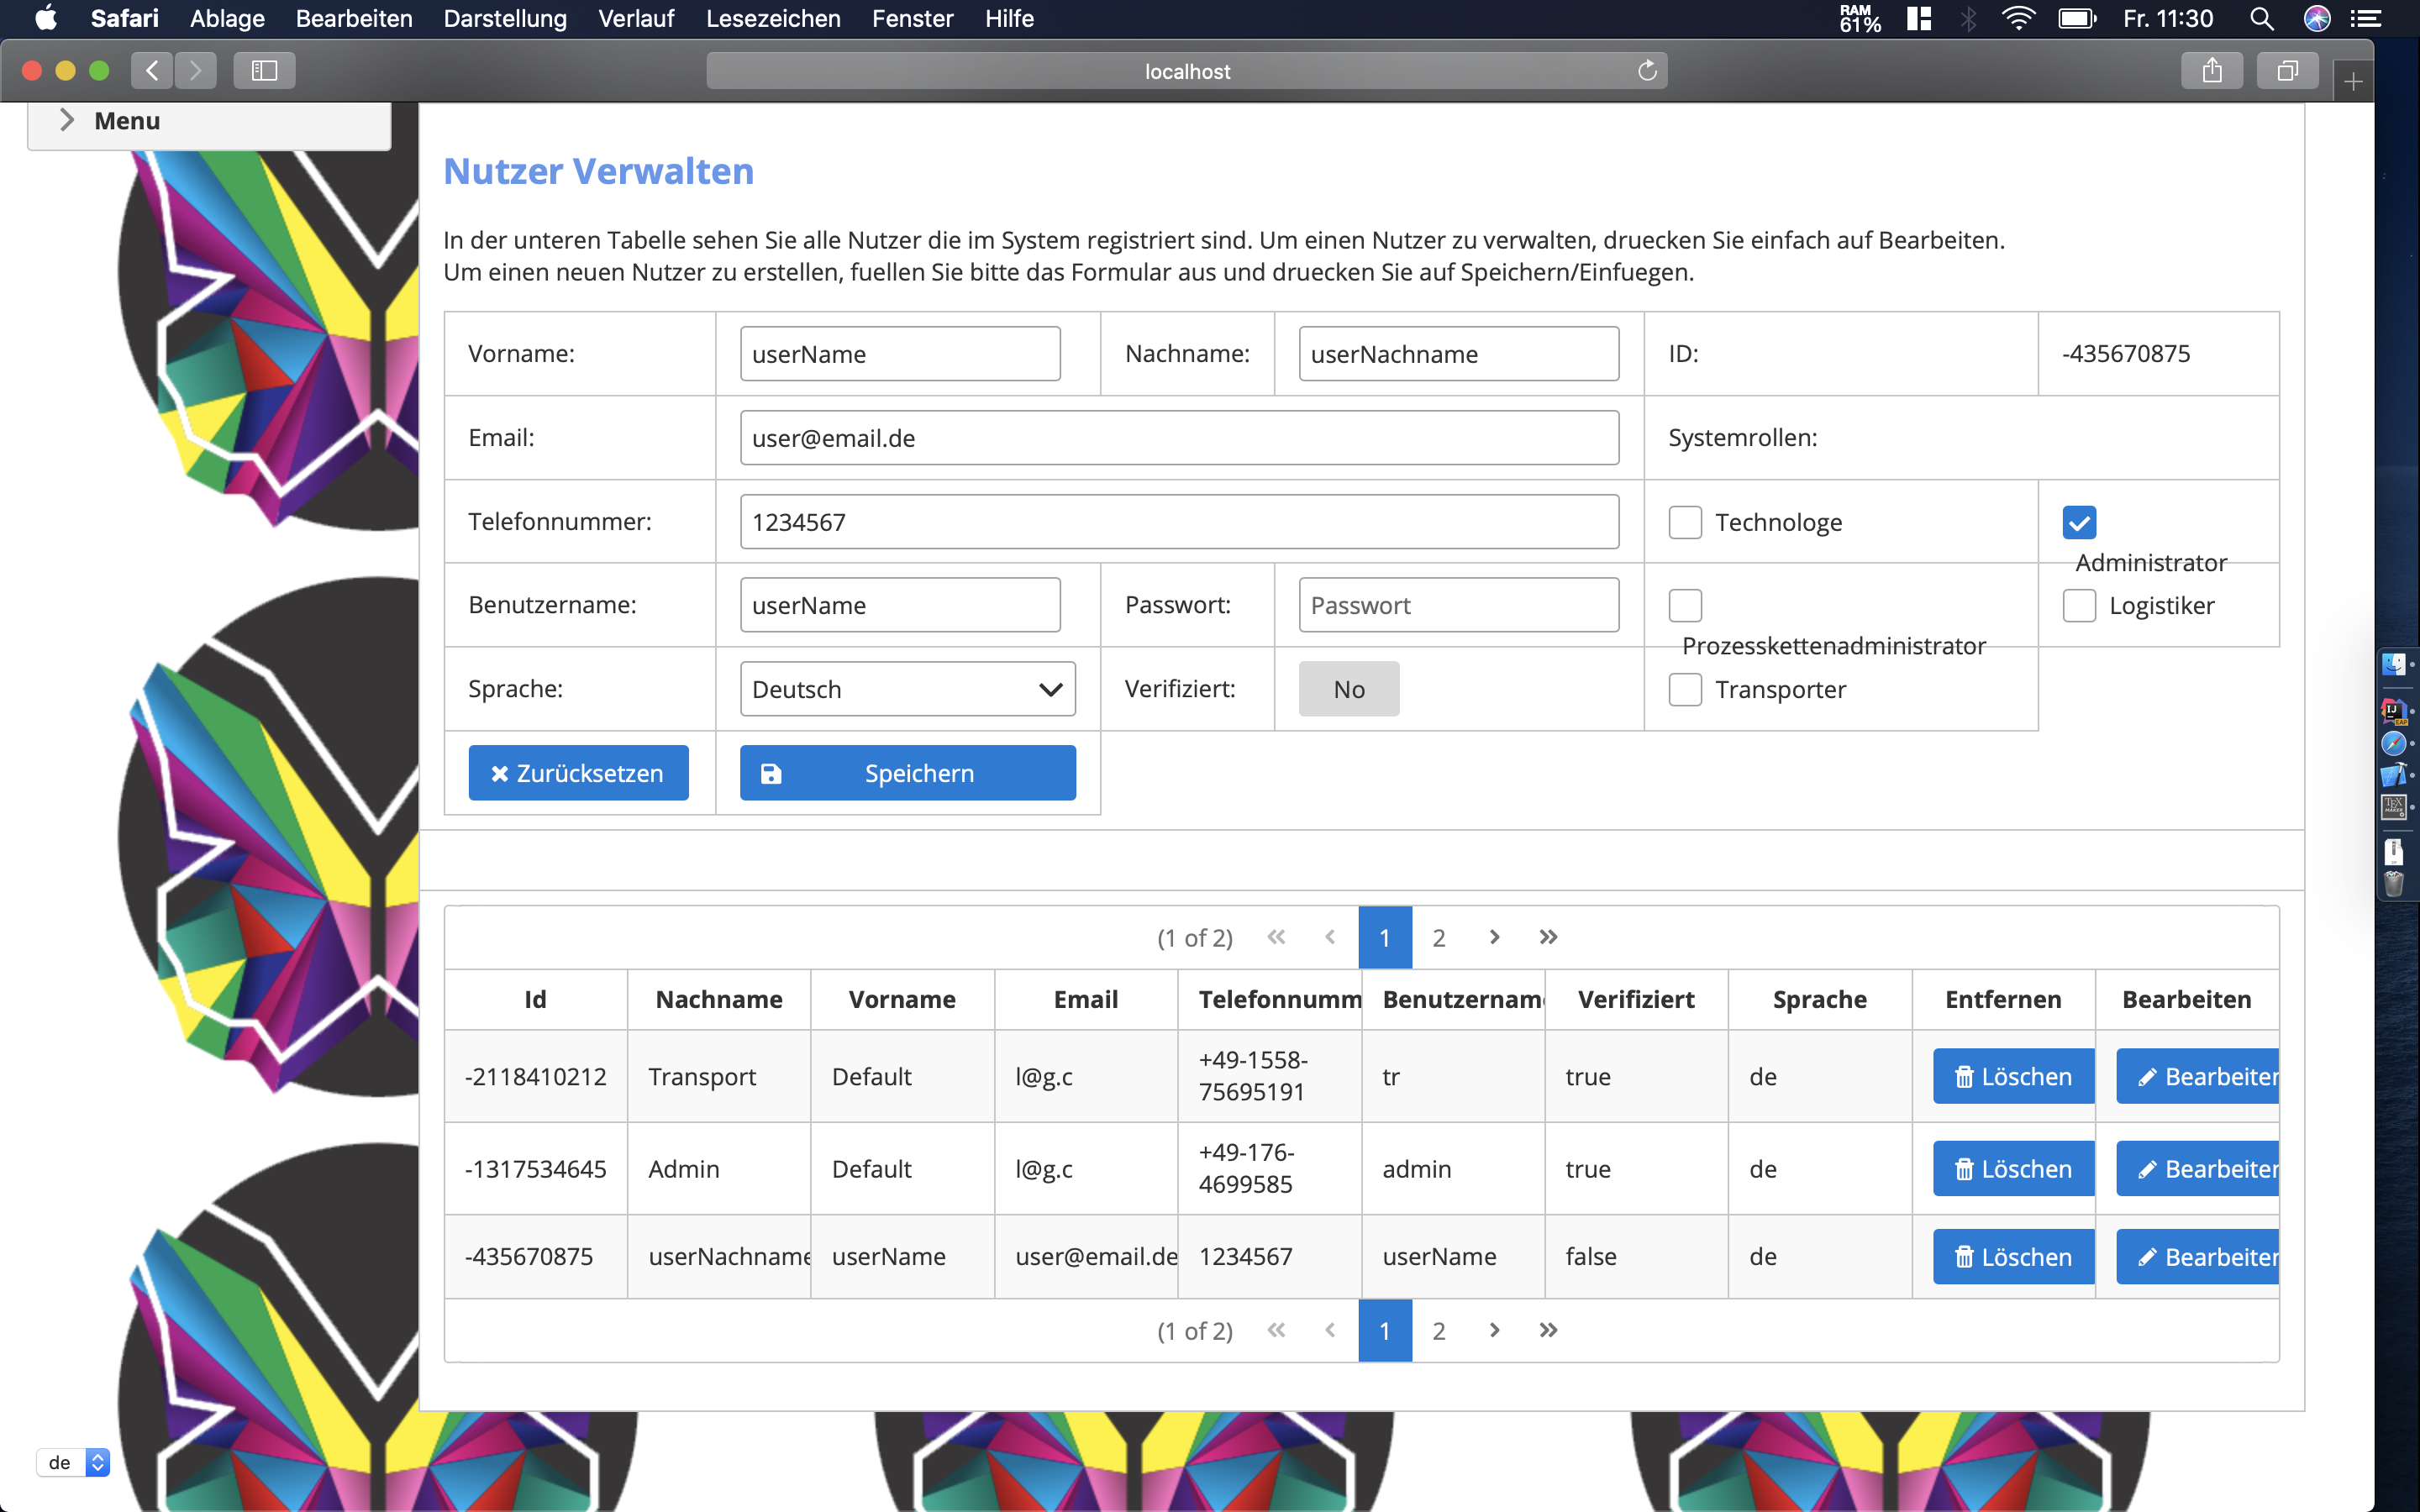
\includegraphics[width=1\textwidth]{Screenshots/userErzeugungInitialData.png}
\textit{Abbildung 3.1.1.9: Pruebe Data für ein neues Benutzer}
} \\
nach dem Drücken der Speichern-Taste. Wir erhalten eine Bestätigung der Software, dass der Benutzer erfolgreich gespeichert wurde.
%%ErzeugunMeldung
\hypertarget{sc3.1.2.3}{
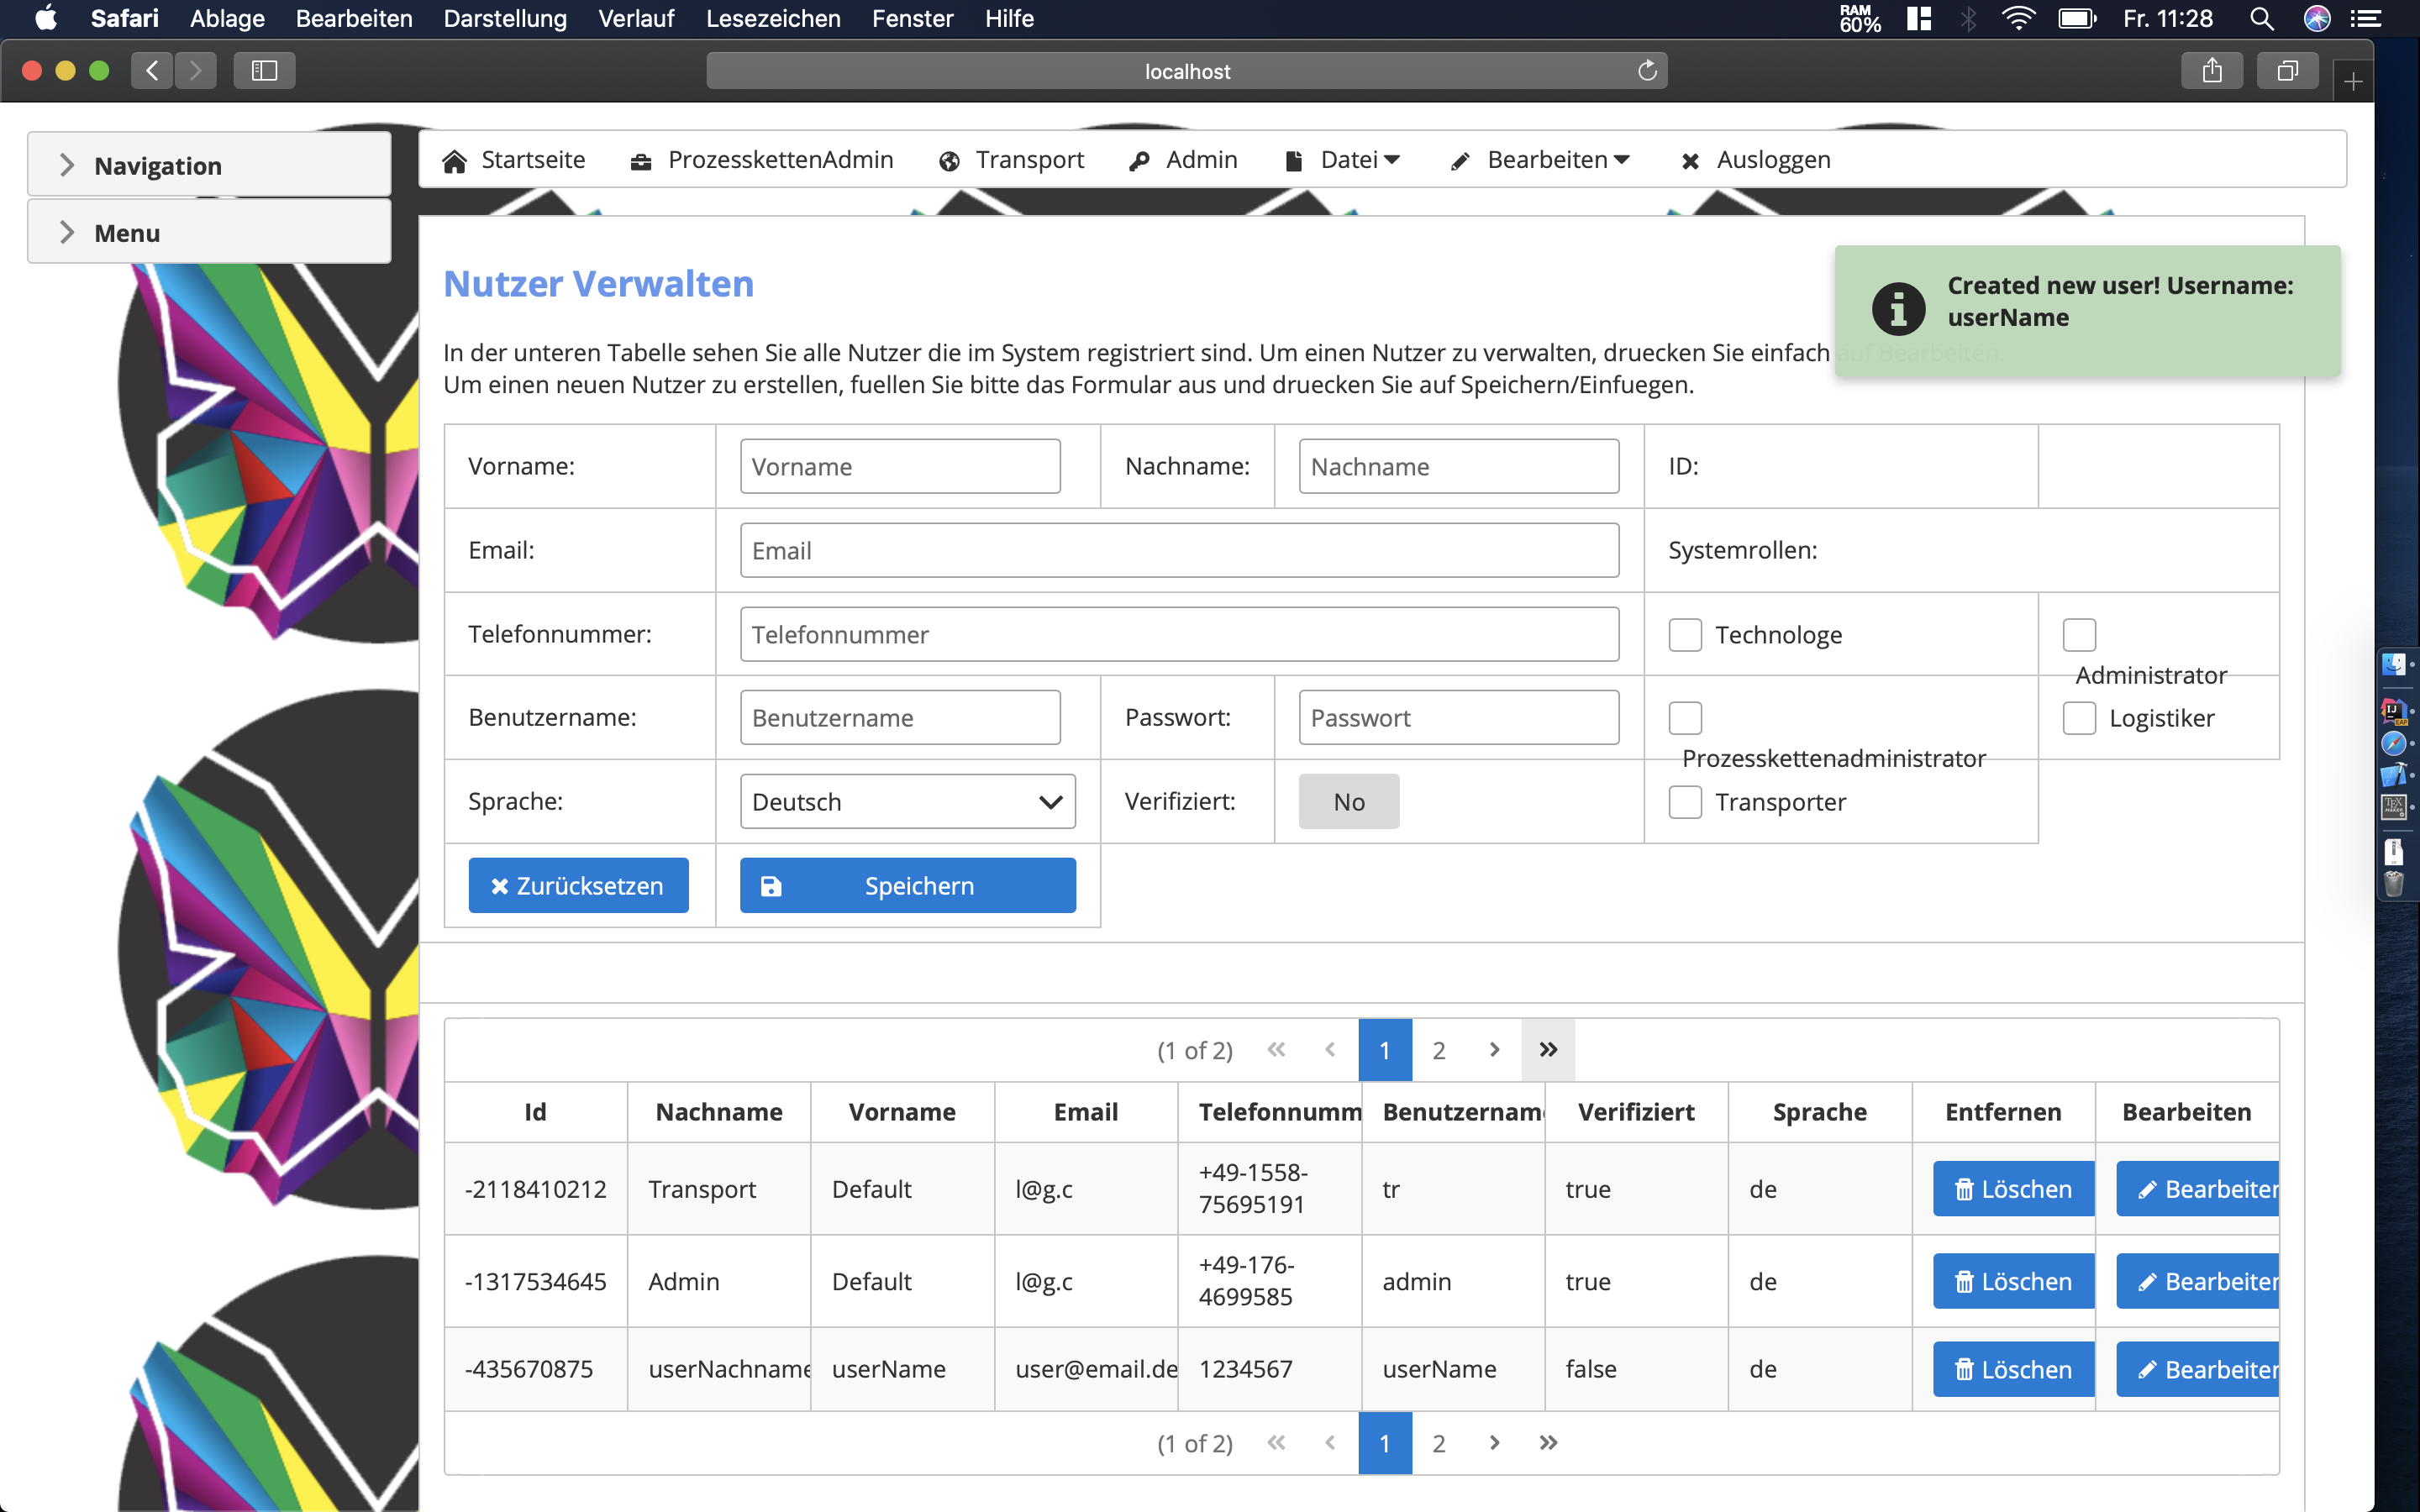
\includegraphics[width=1\textwidth]{Screenshots/userErzeugenMeldung.png}
\textit{Abbildung 3.1.1.10: Meldung von neuer Benutzer an der Webseite}
} \\

Um die spezifischen Informationen zuvor gespeicherter Benutzer zu bearbeiten, drücken Sie die Taste Bwerden. Bearbeiten Sie anschließend die Daten im Formular und klicken Sie abschließend auf die Schaltfläche Speichern.
%%Bearbeiten
\hypertarget{sc3.1.2.4}{
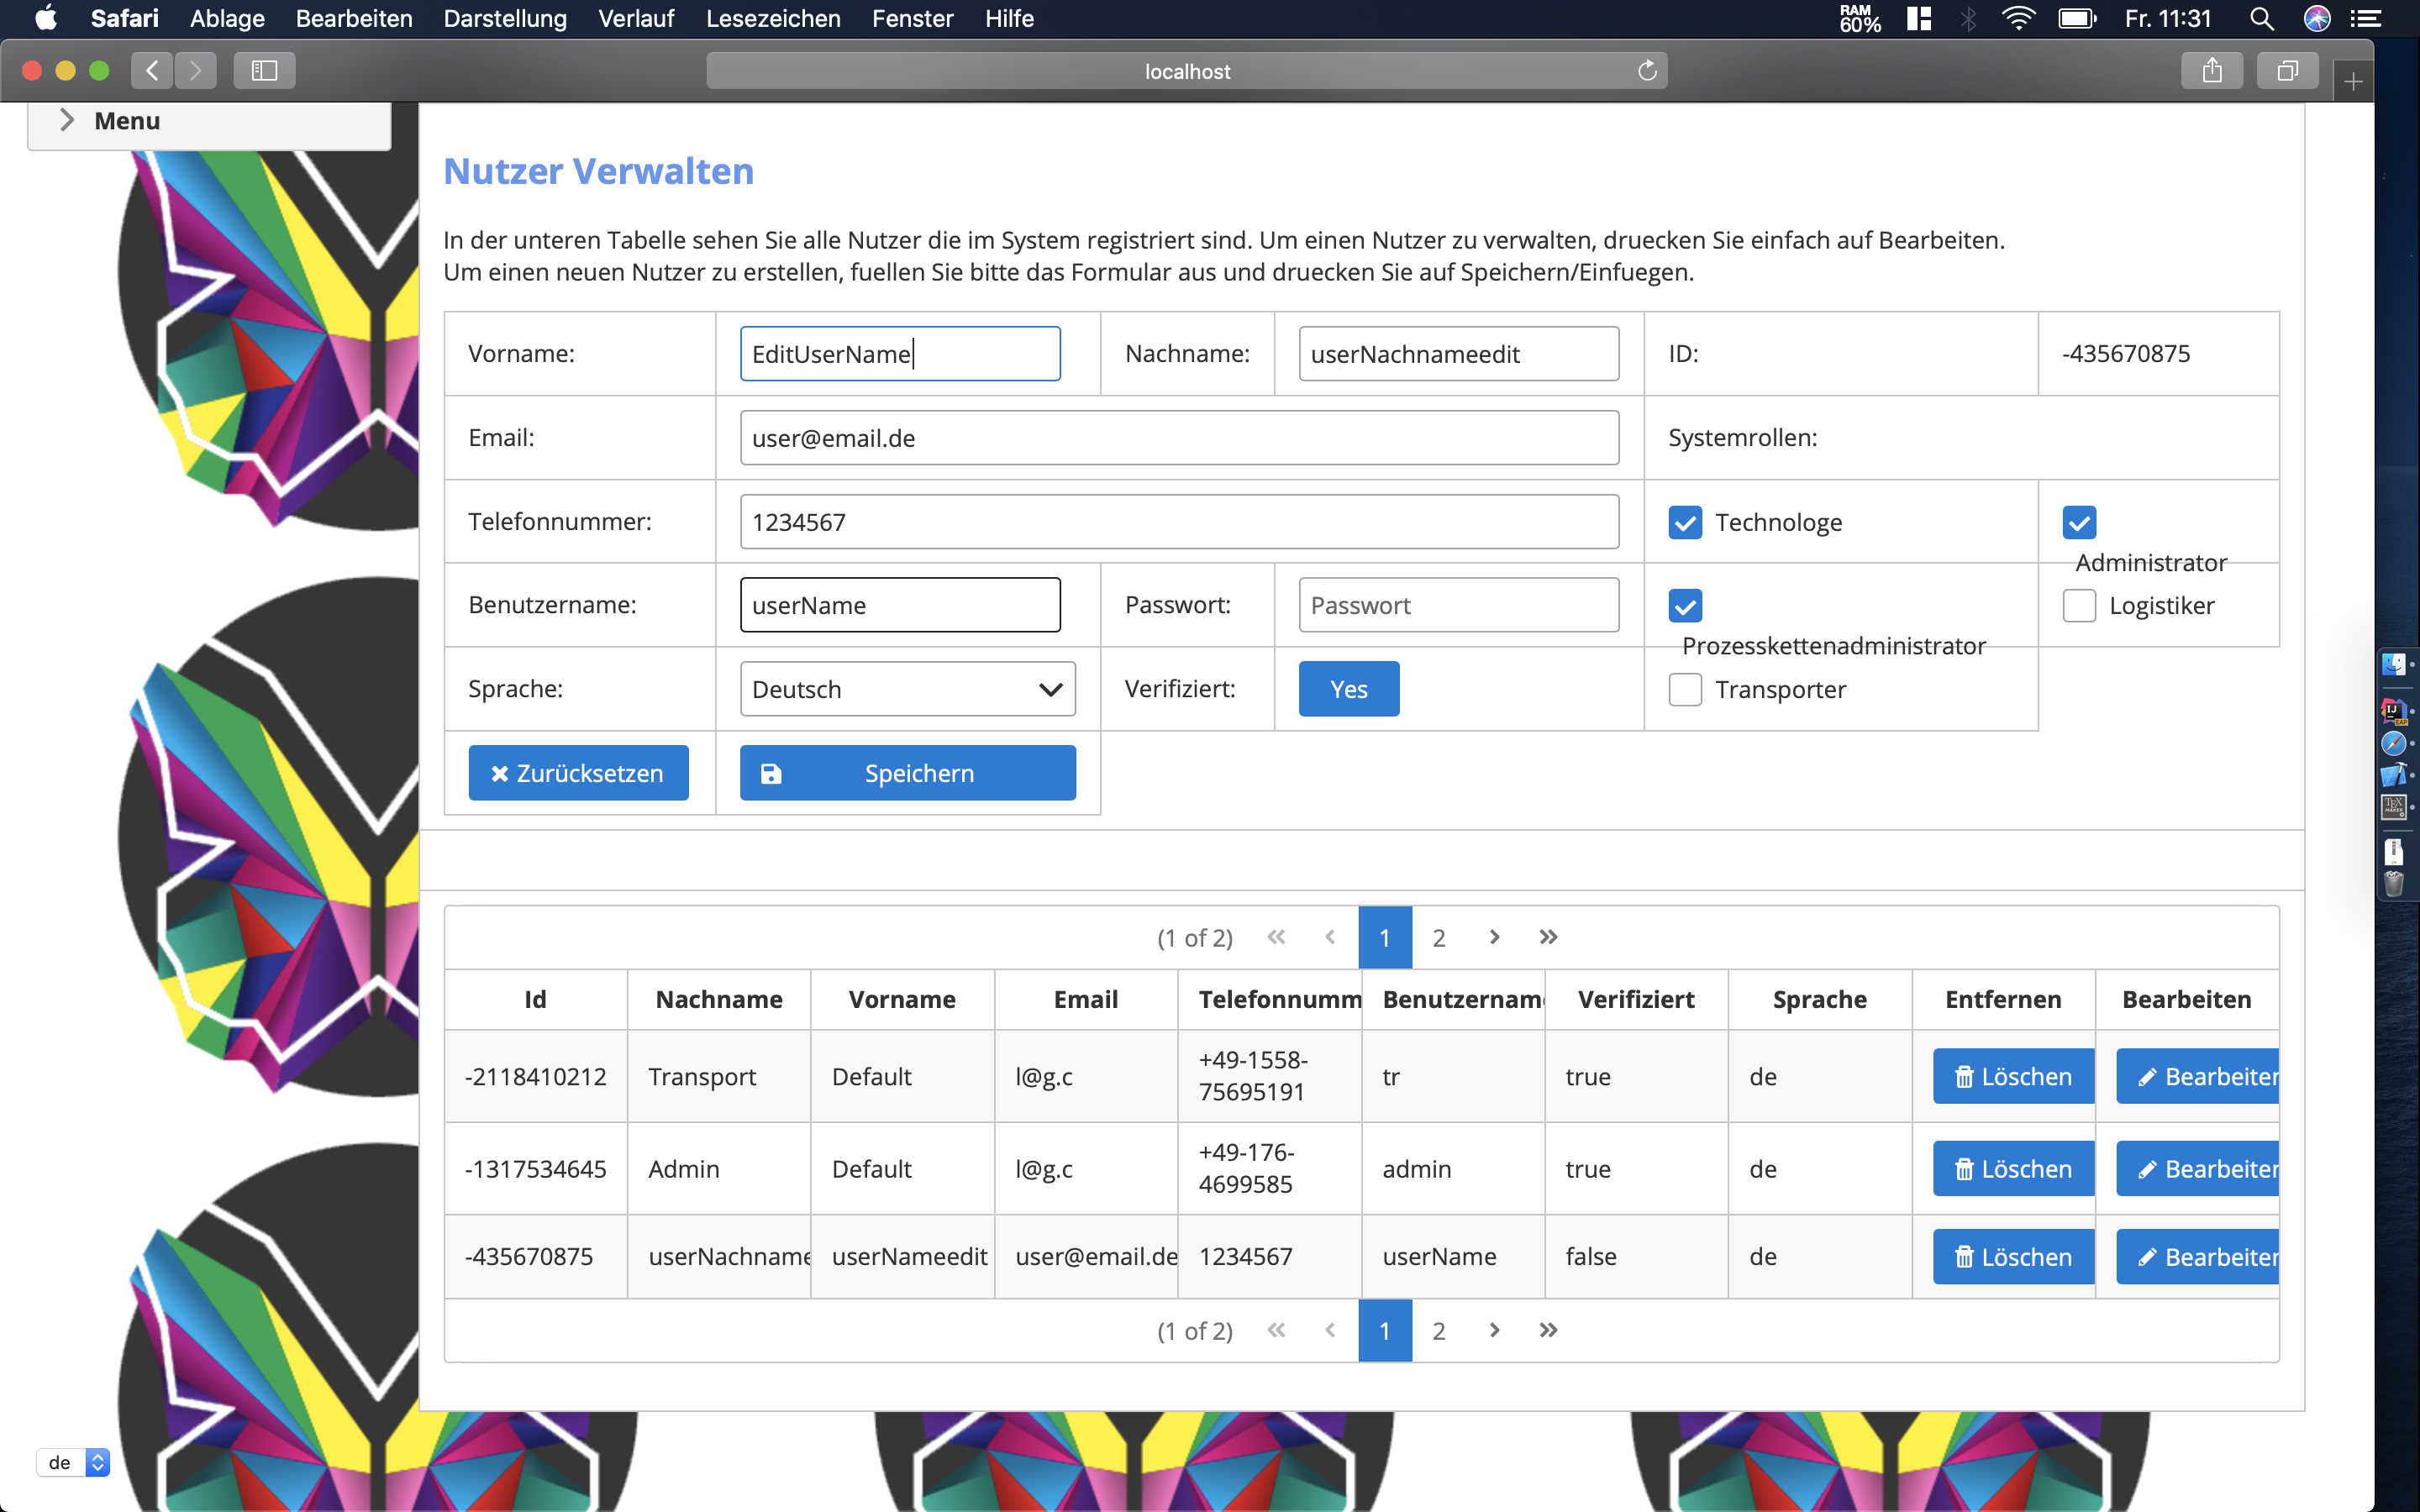
\includegraphics[width=1\textwidth]{Screenshots/UserEditData.png}
\textit{Abbildung 3.1.1.11: Bearbeitung von Data an der Pruebe Benutzer}
} \\
Nachdem der Benutzer gespeichert wurde, sendet die Website eine Bestätigungsnachricht. Wenn inkonsistente Daten eingegeben werden, sendet die Website eine Misserfolgsnachricht.
%%Editmeldung
\hypertarget{sc3.1.2.5}{
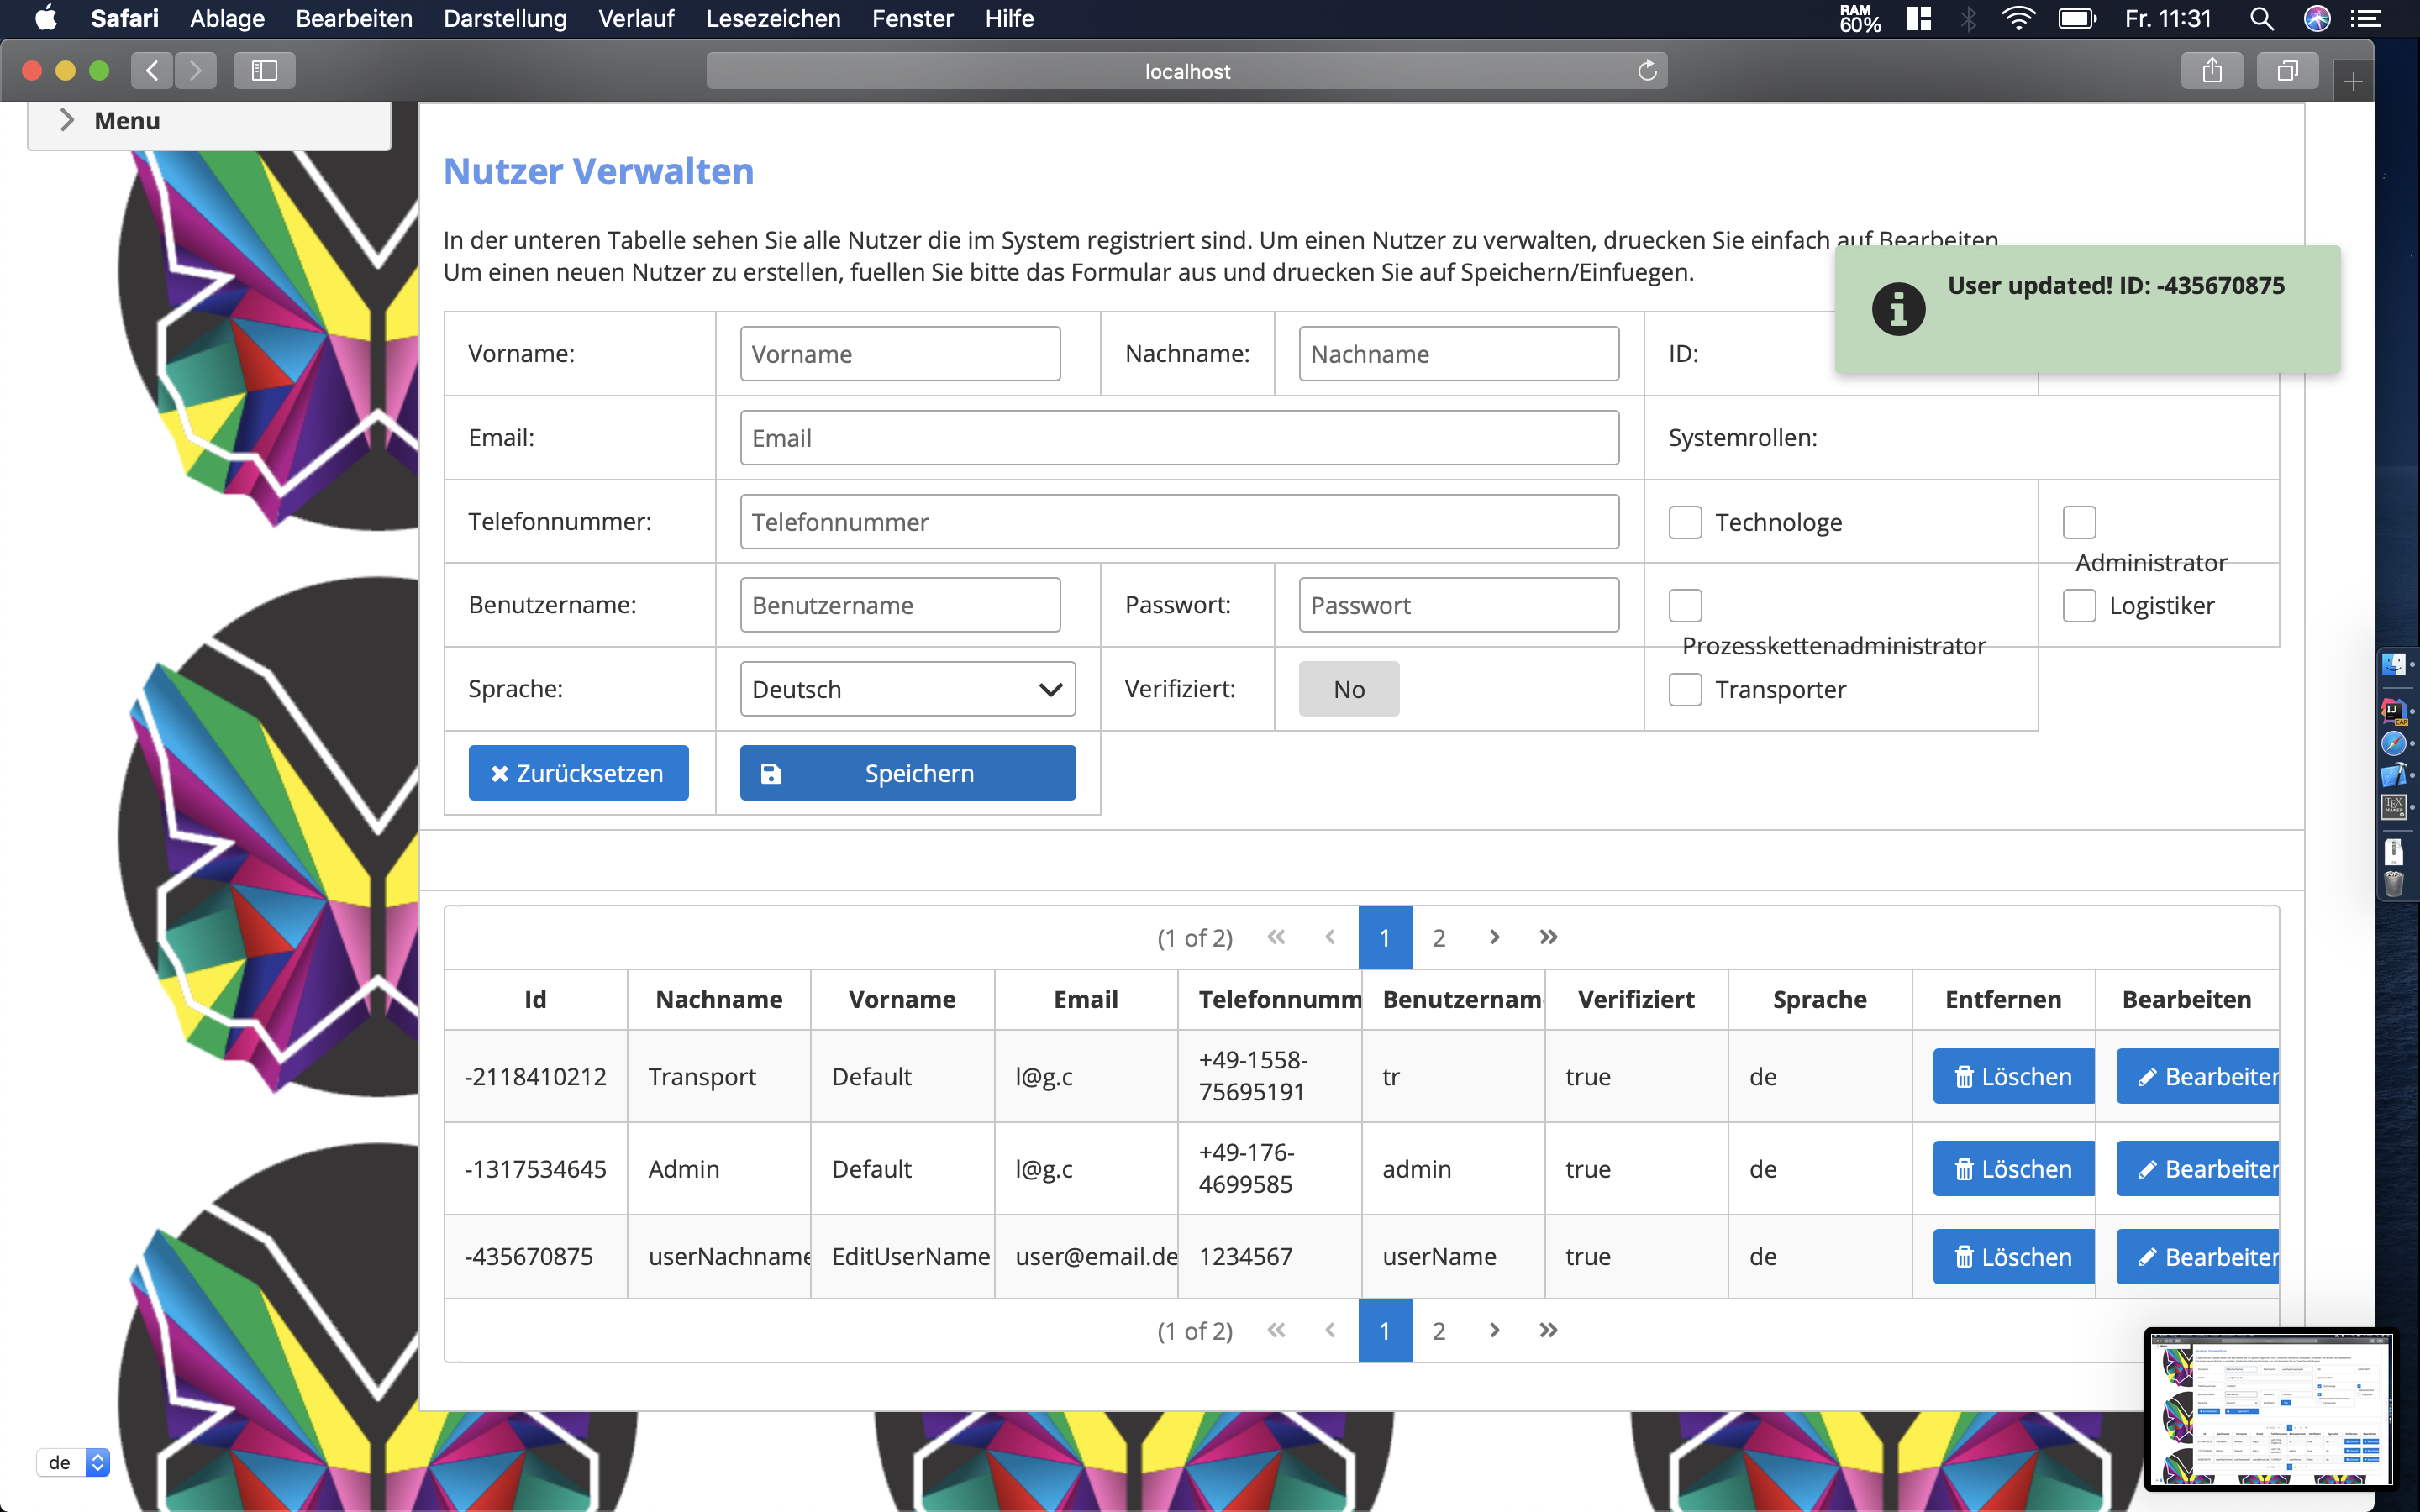
\includegraphics[width=1\textwidth]{Screenshots/editMeldung.png}
\textit{Abbildung 3.1.1.12: Meldung von Erfolgreiche Bearbeitung der Data von nutzer}
} \\


Nachdem der Benutzer editiert wurde, sendet die Website eine Bestätigungsnachricht.
%%InconsistenceData
\hypertarget{sc3.1.2.6}{
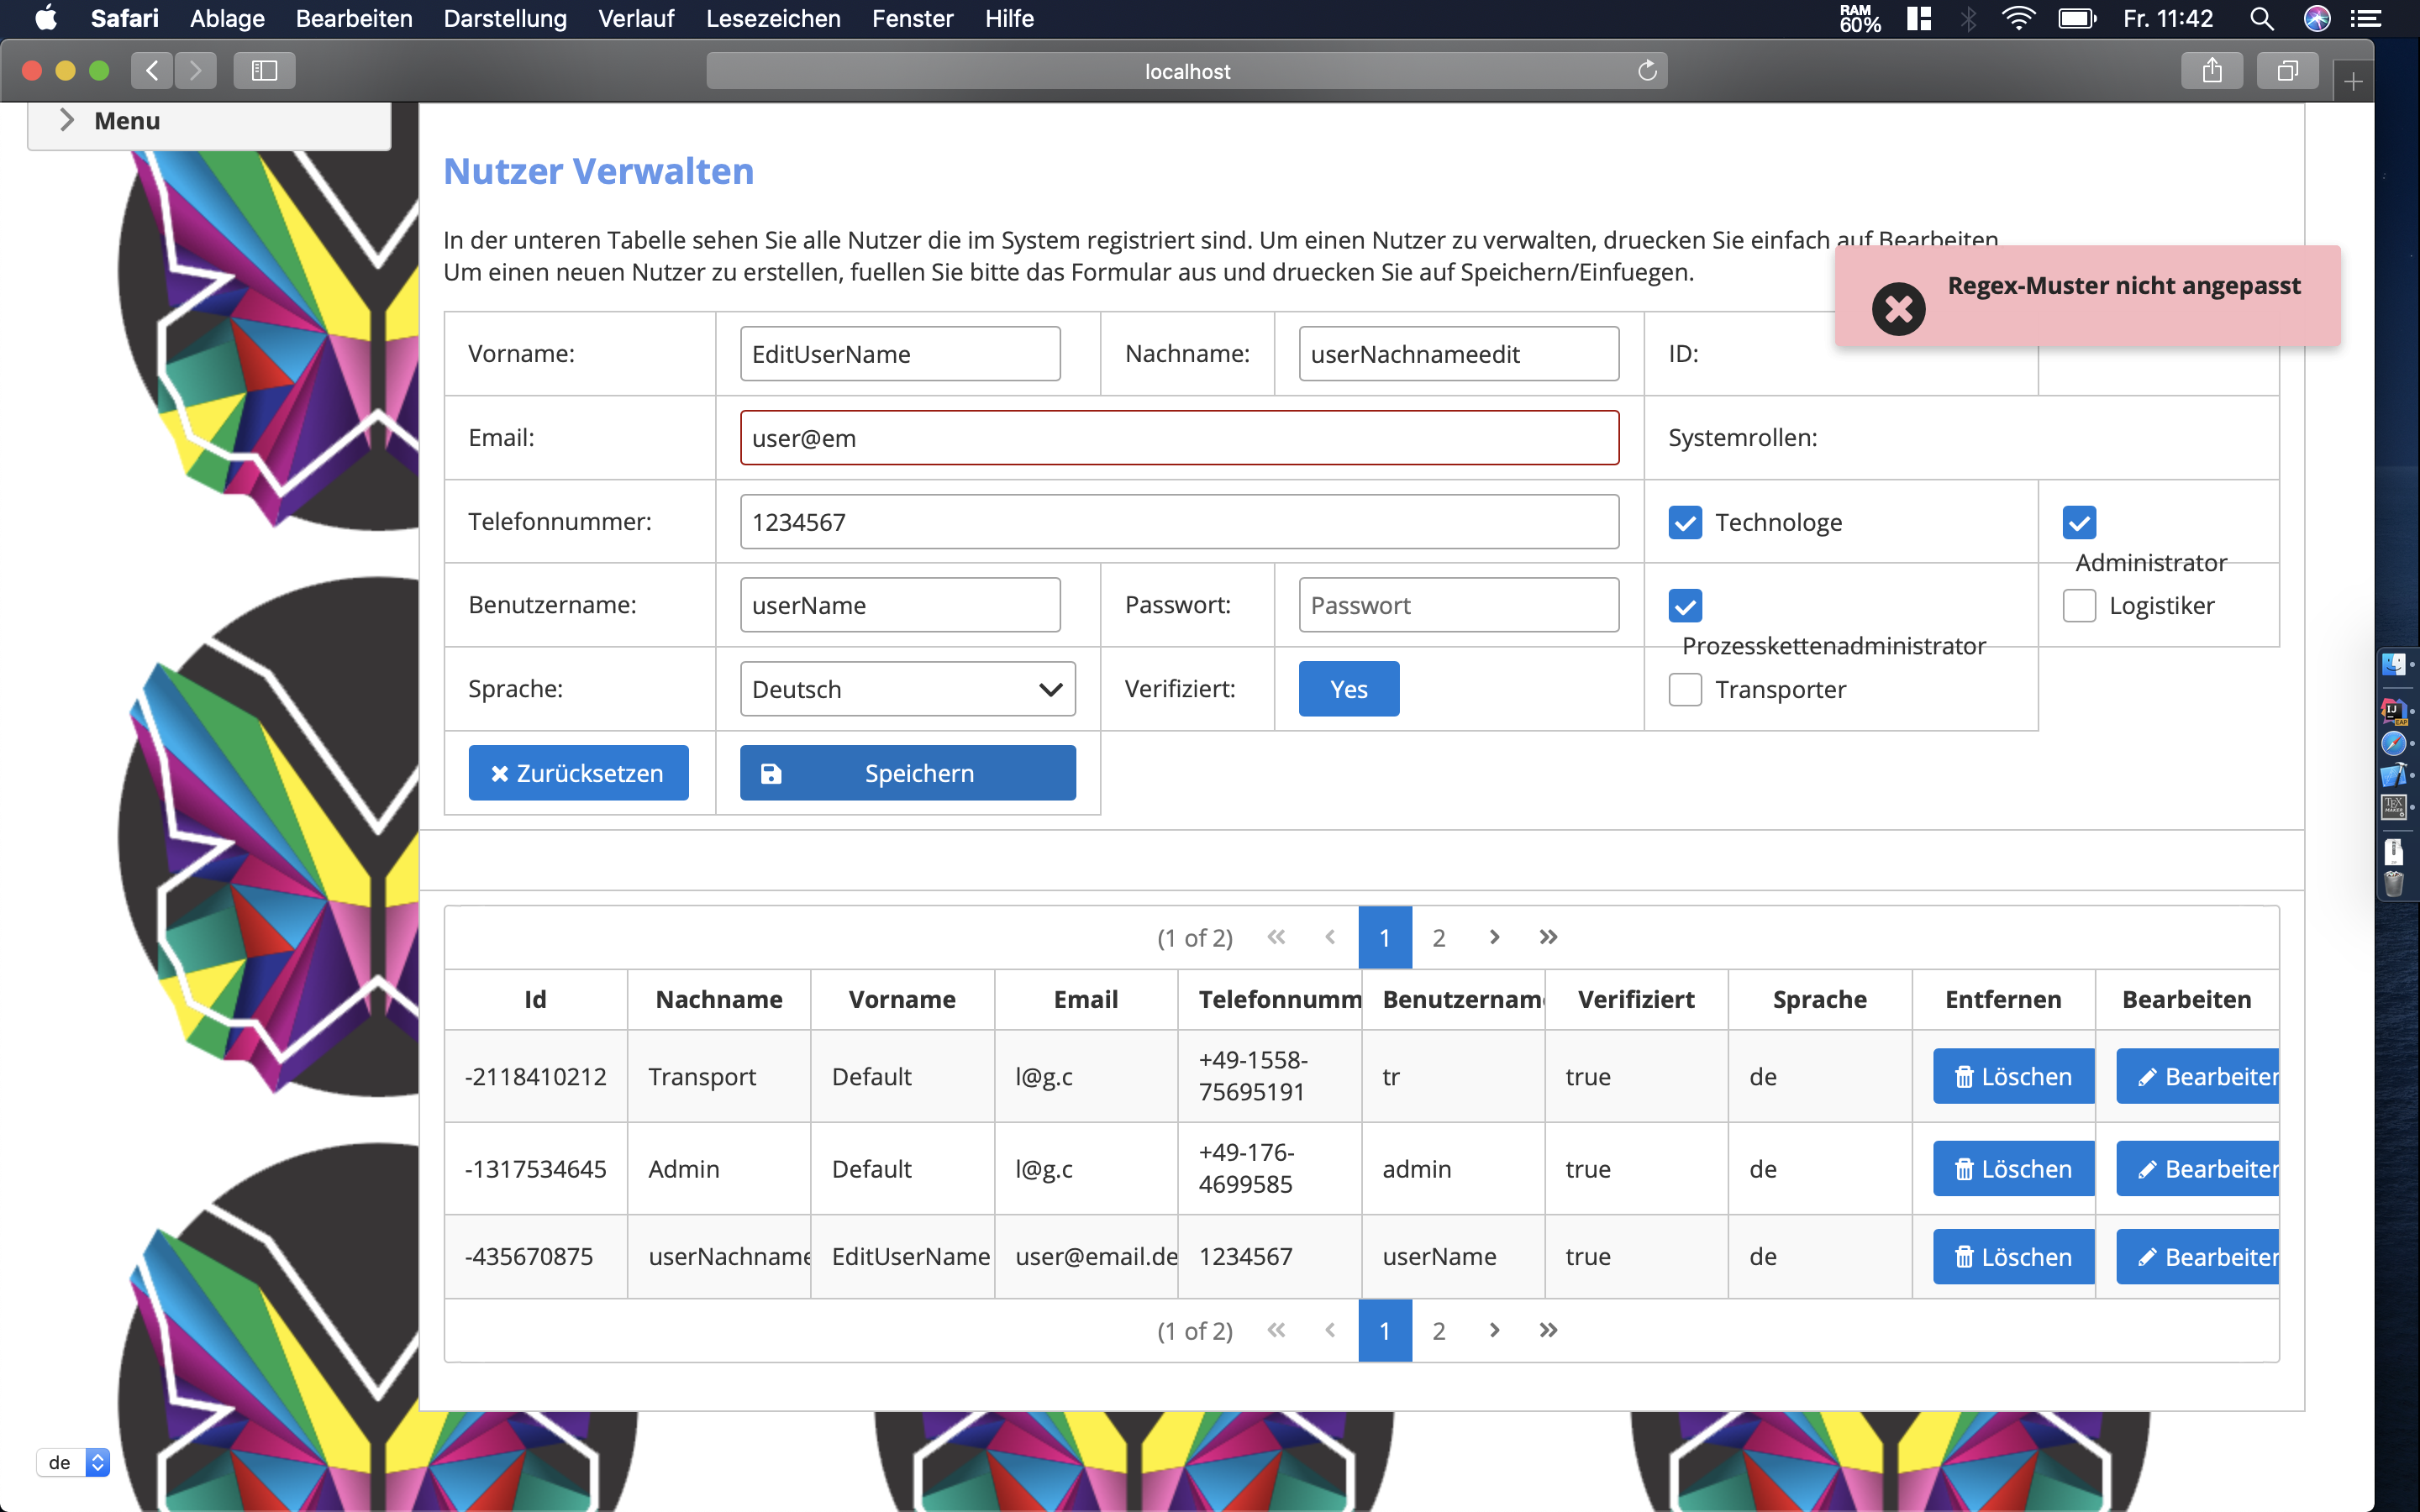
\includegraphics[width=1\textwidth]{Screenshots/InconsistenceDataUserBearbeitung.png}
\textit{Abbildung 3.1.1.13: Meldung von Erfolgreiche Bearbeitung der Data von nutzer}
} \\
Wenn Benutzer gelöscht werden, wird eine Bestätigungsnachricht von der Website abgerufen und der Benutzer wird aus der Benutzertabelle entfernt.
\hypertarget{sc3.1.2.7}{
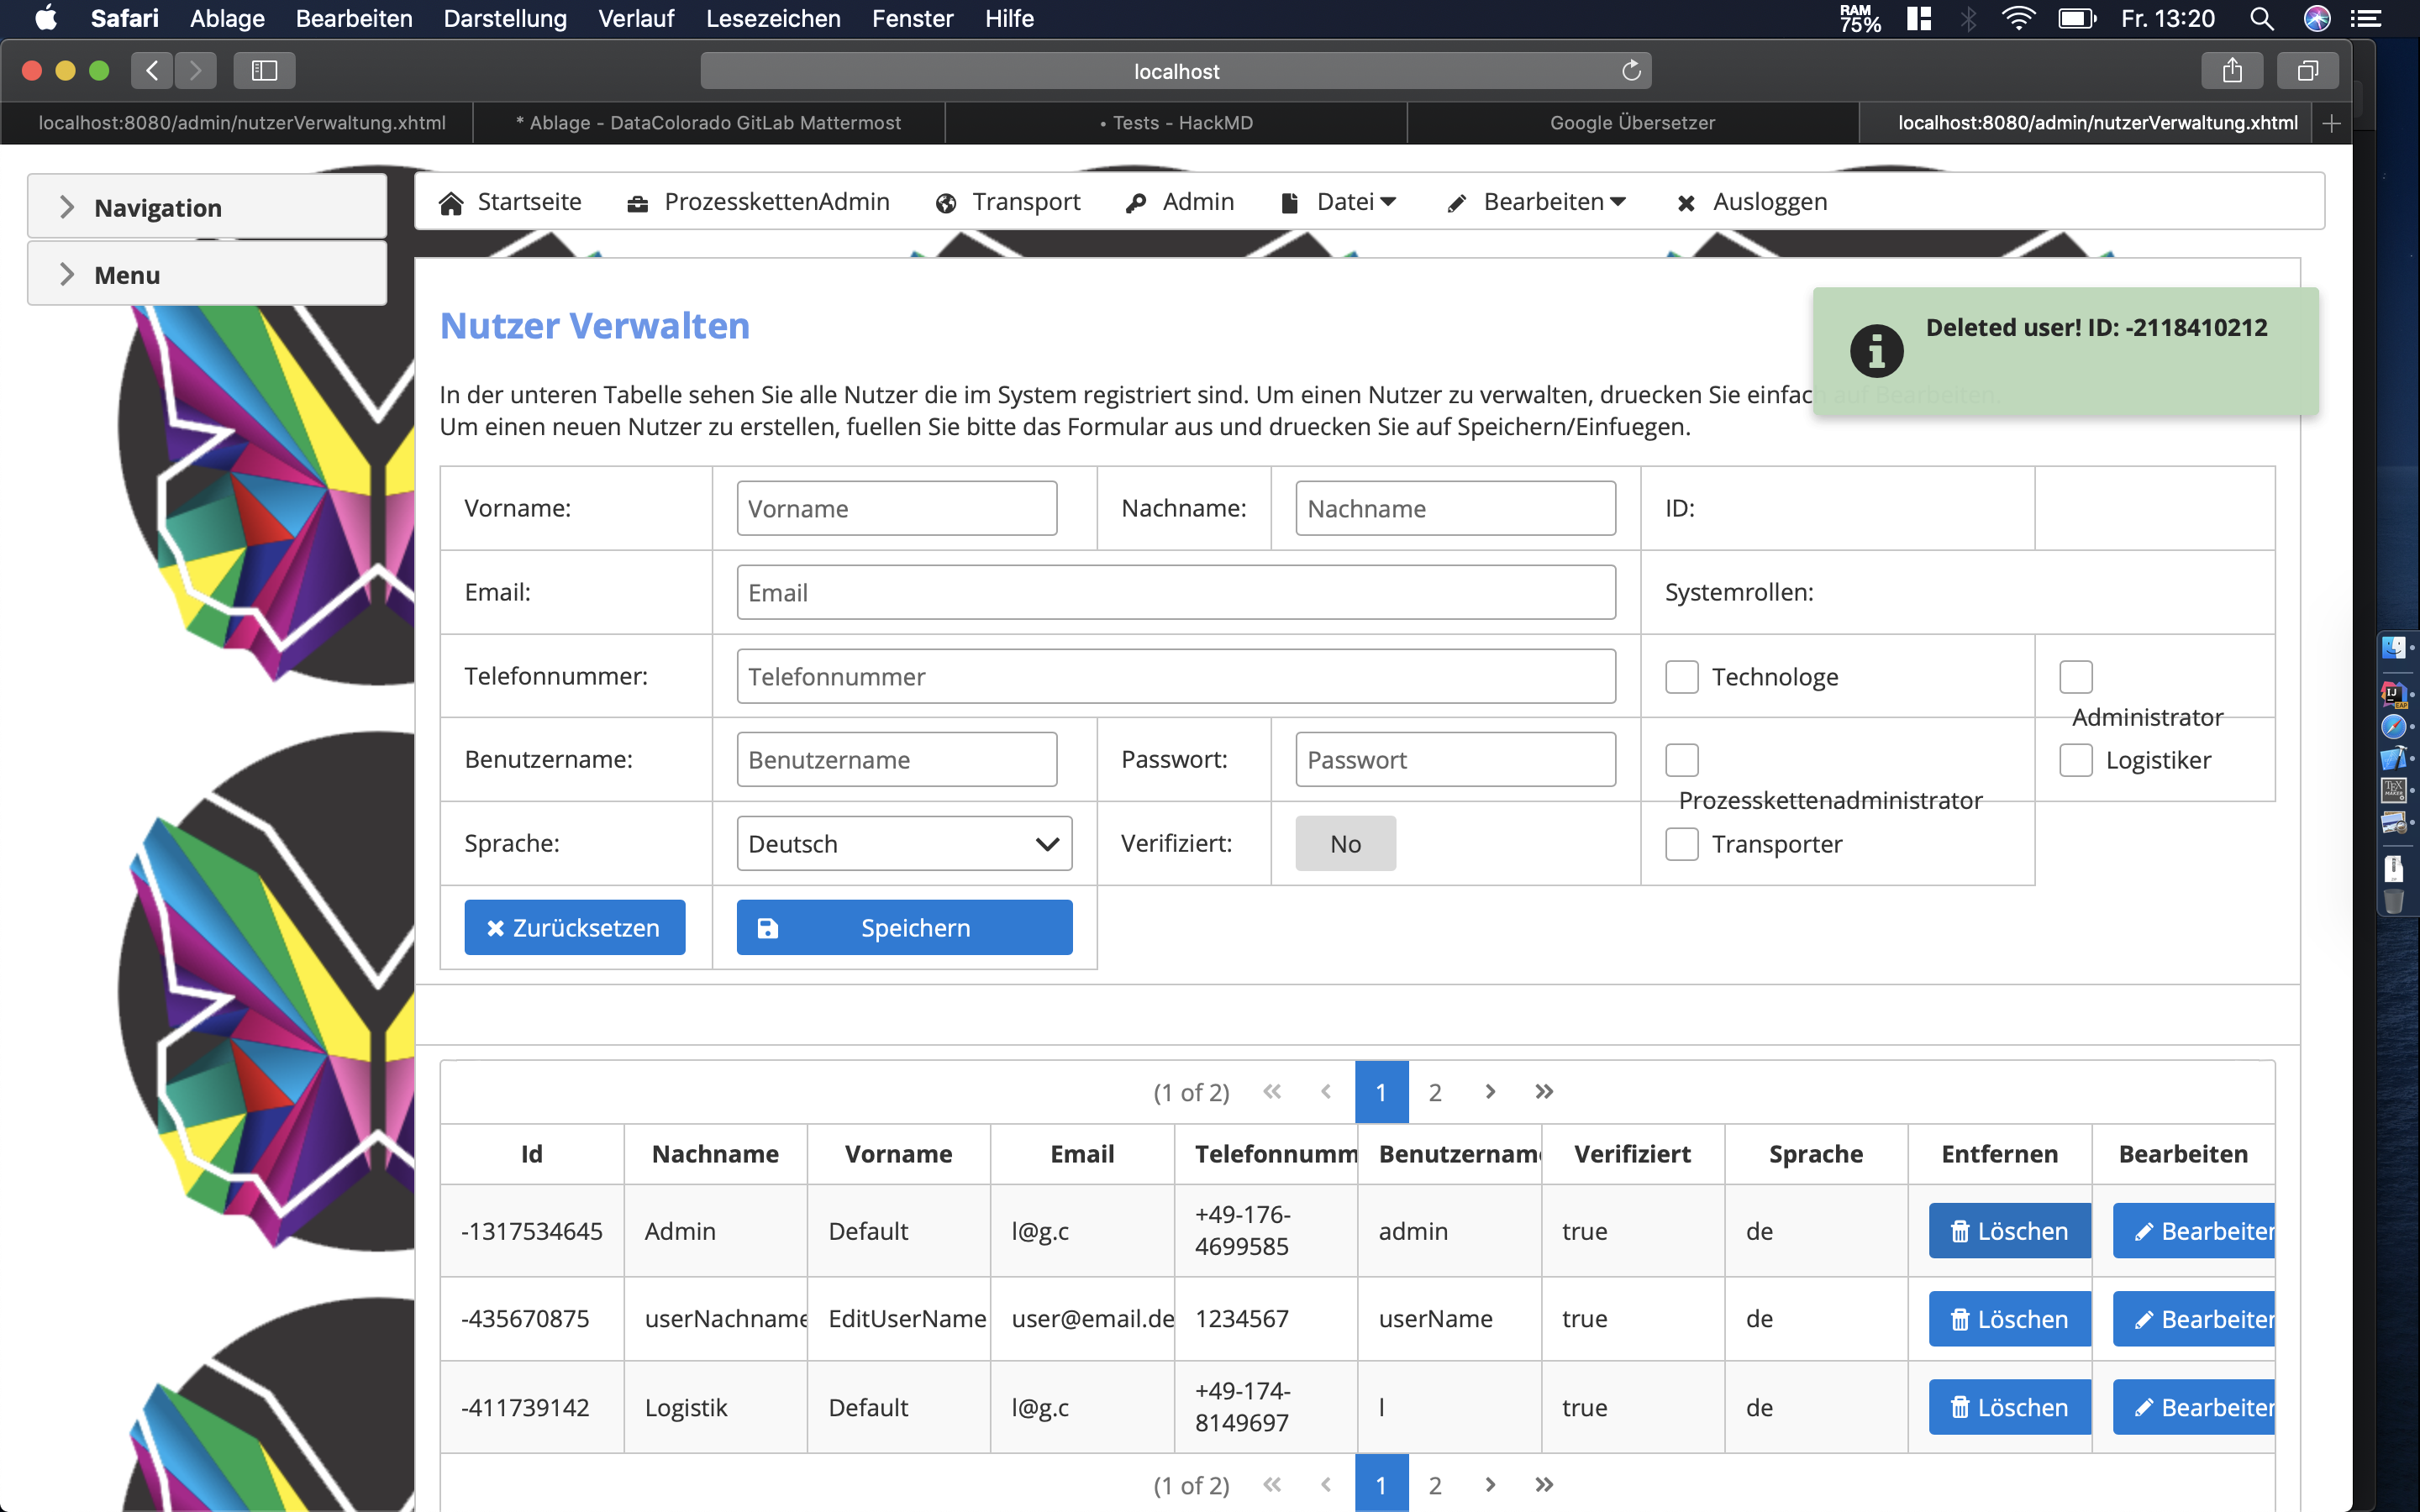
\includegraphics[width=1\textwidth]{Screenshots/BenutzerEntfernen.png}
\textit{Abbildung 3.1.1.13: Meldung von Erfolgreiche Bearbeitung der Data von nutzer}
} \\
%%

\subsubsection{Anwendungsfall: Admin verwaltet Experimentierstation}

Der Admin startet auf seiner \hyperlink{sc3.1.3.1}{Startseite}, nachdem er sich eingeloggt hat. \\

\hypertarget{sc3.1.3.1}{
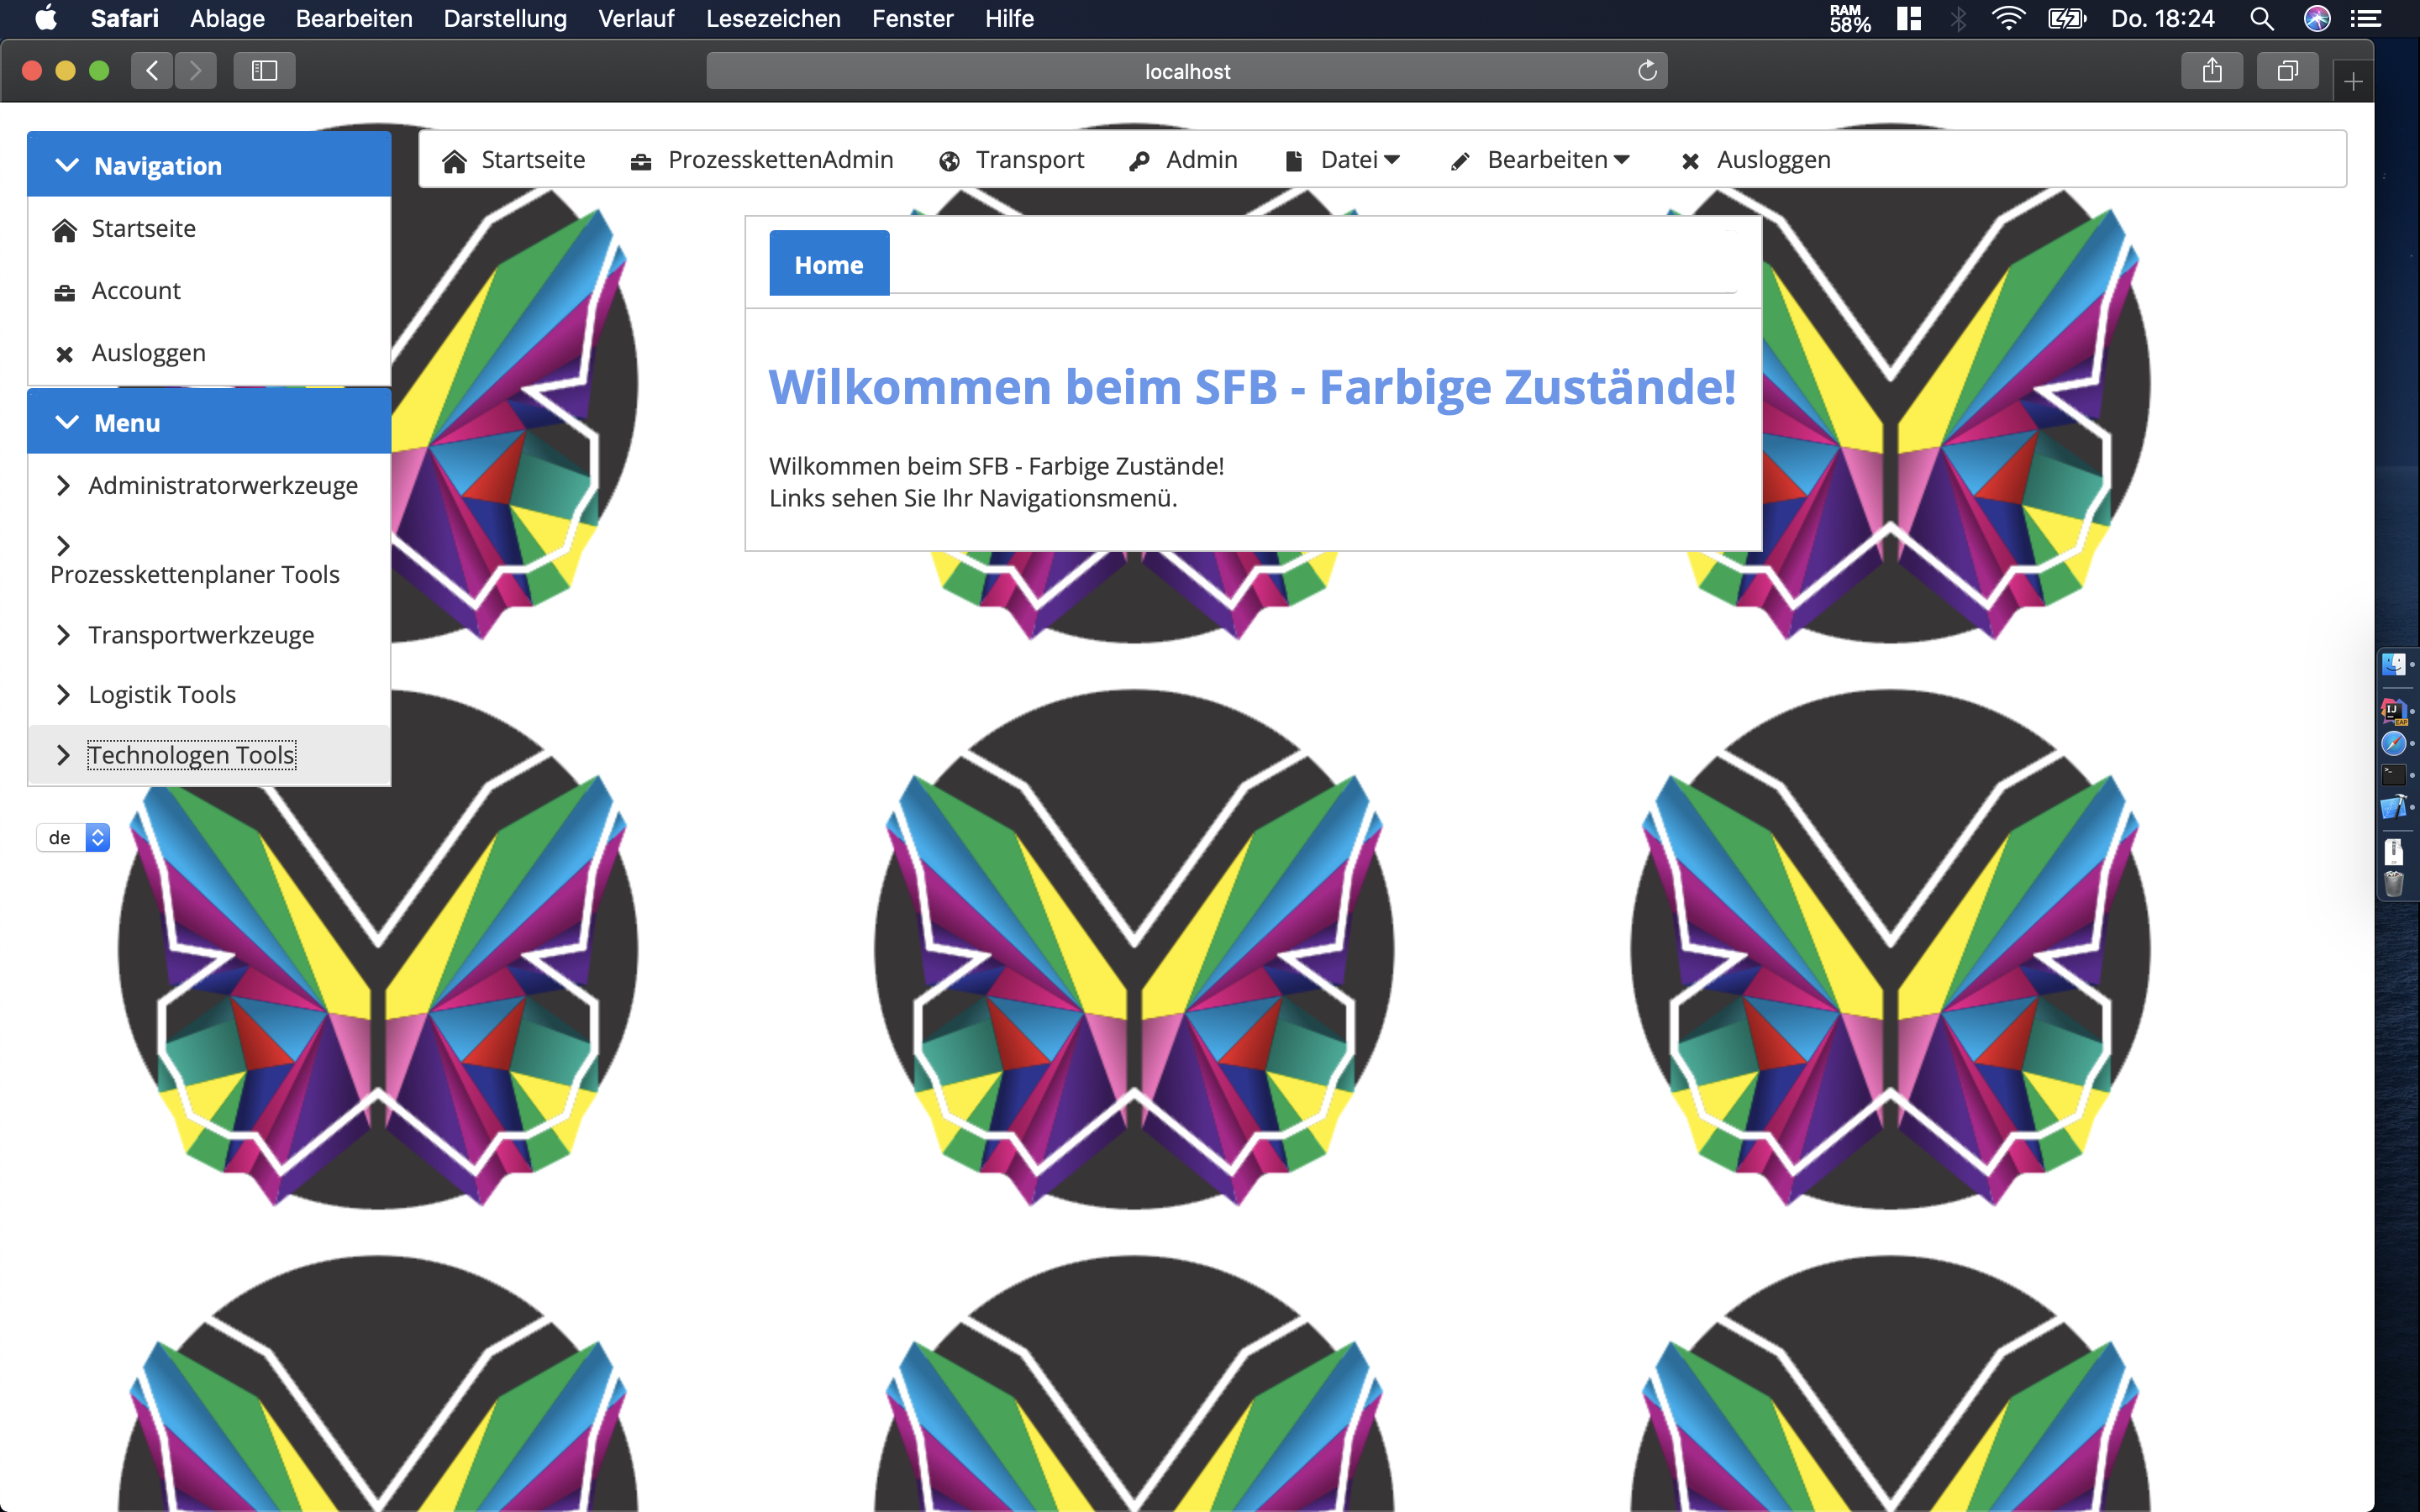
\includegraphics[width=1\textwidth]{Screenshots/311AdminView.png}
\textit{Abbildung 3.1.3.1: Startseite des Admins}
} \\

Er öffnet das Administratorwerkzeuge Menü am linken Bildschirmrand und drückt auf Experimentierstationen verwalten. Nun wird er auf die Seite zum \hyperlink{sc3.1.3.2}{Verwalten der Experimentierstationen} weitergeleitet. \\

\hypertarget{sc3.1.3.2}{
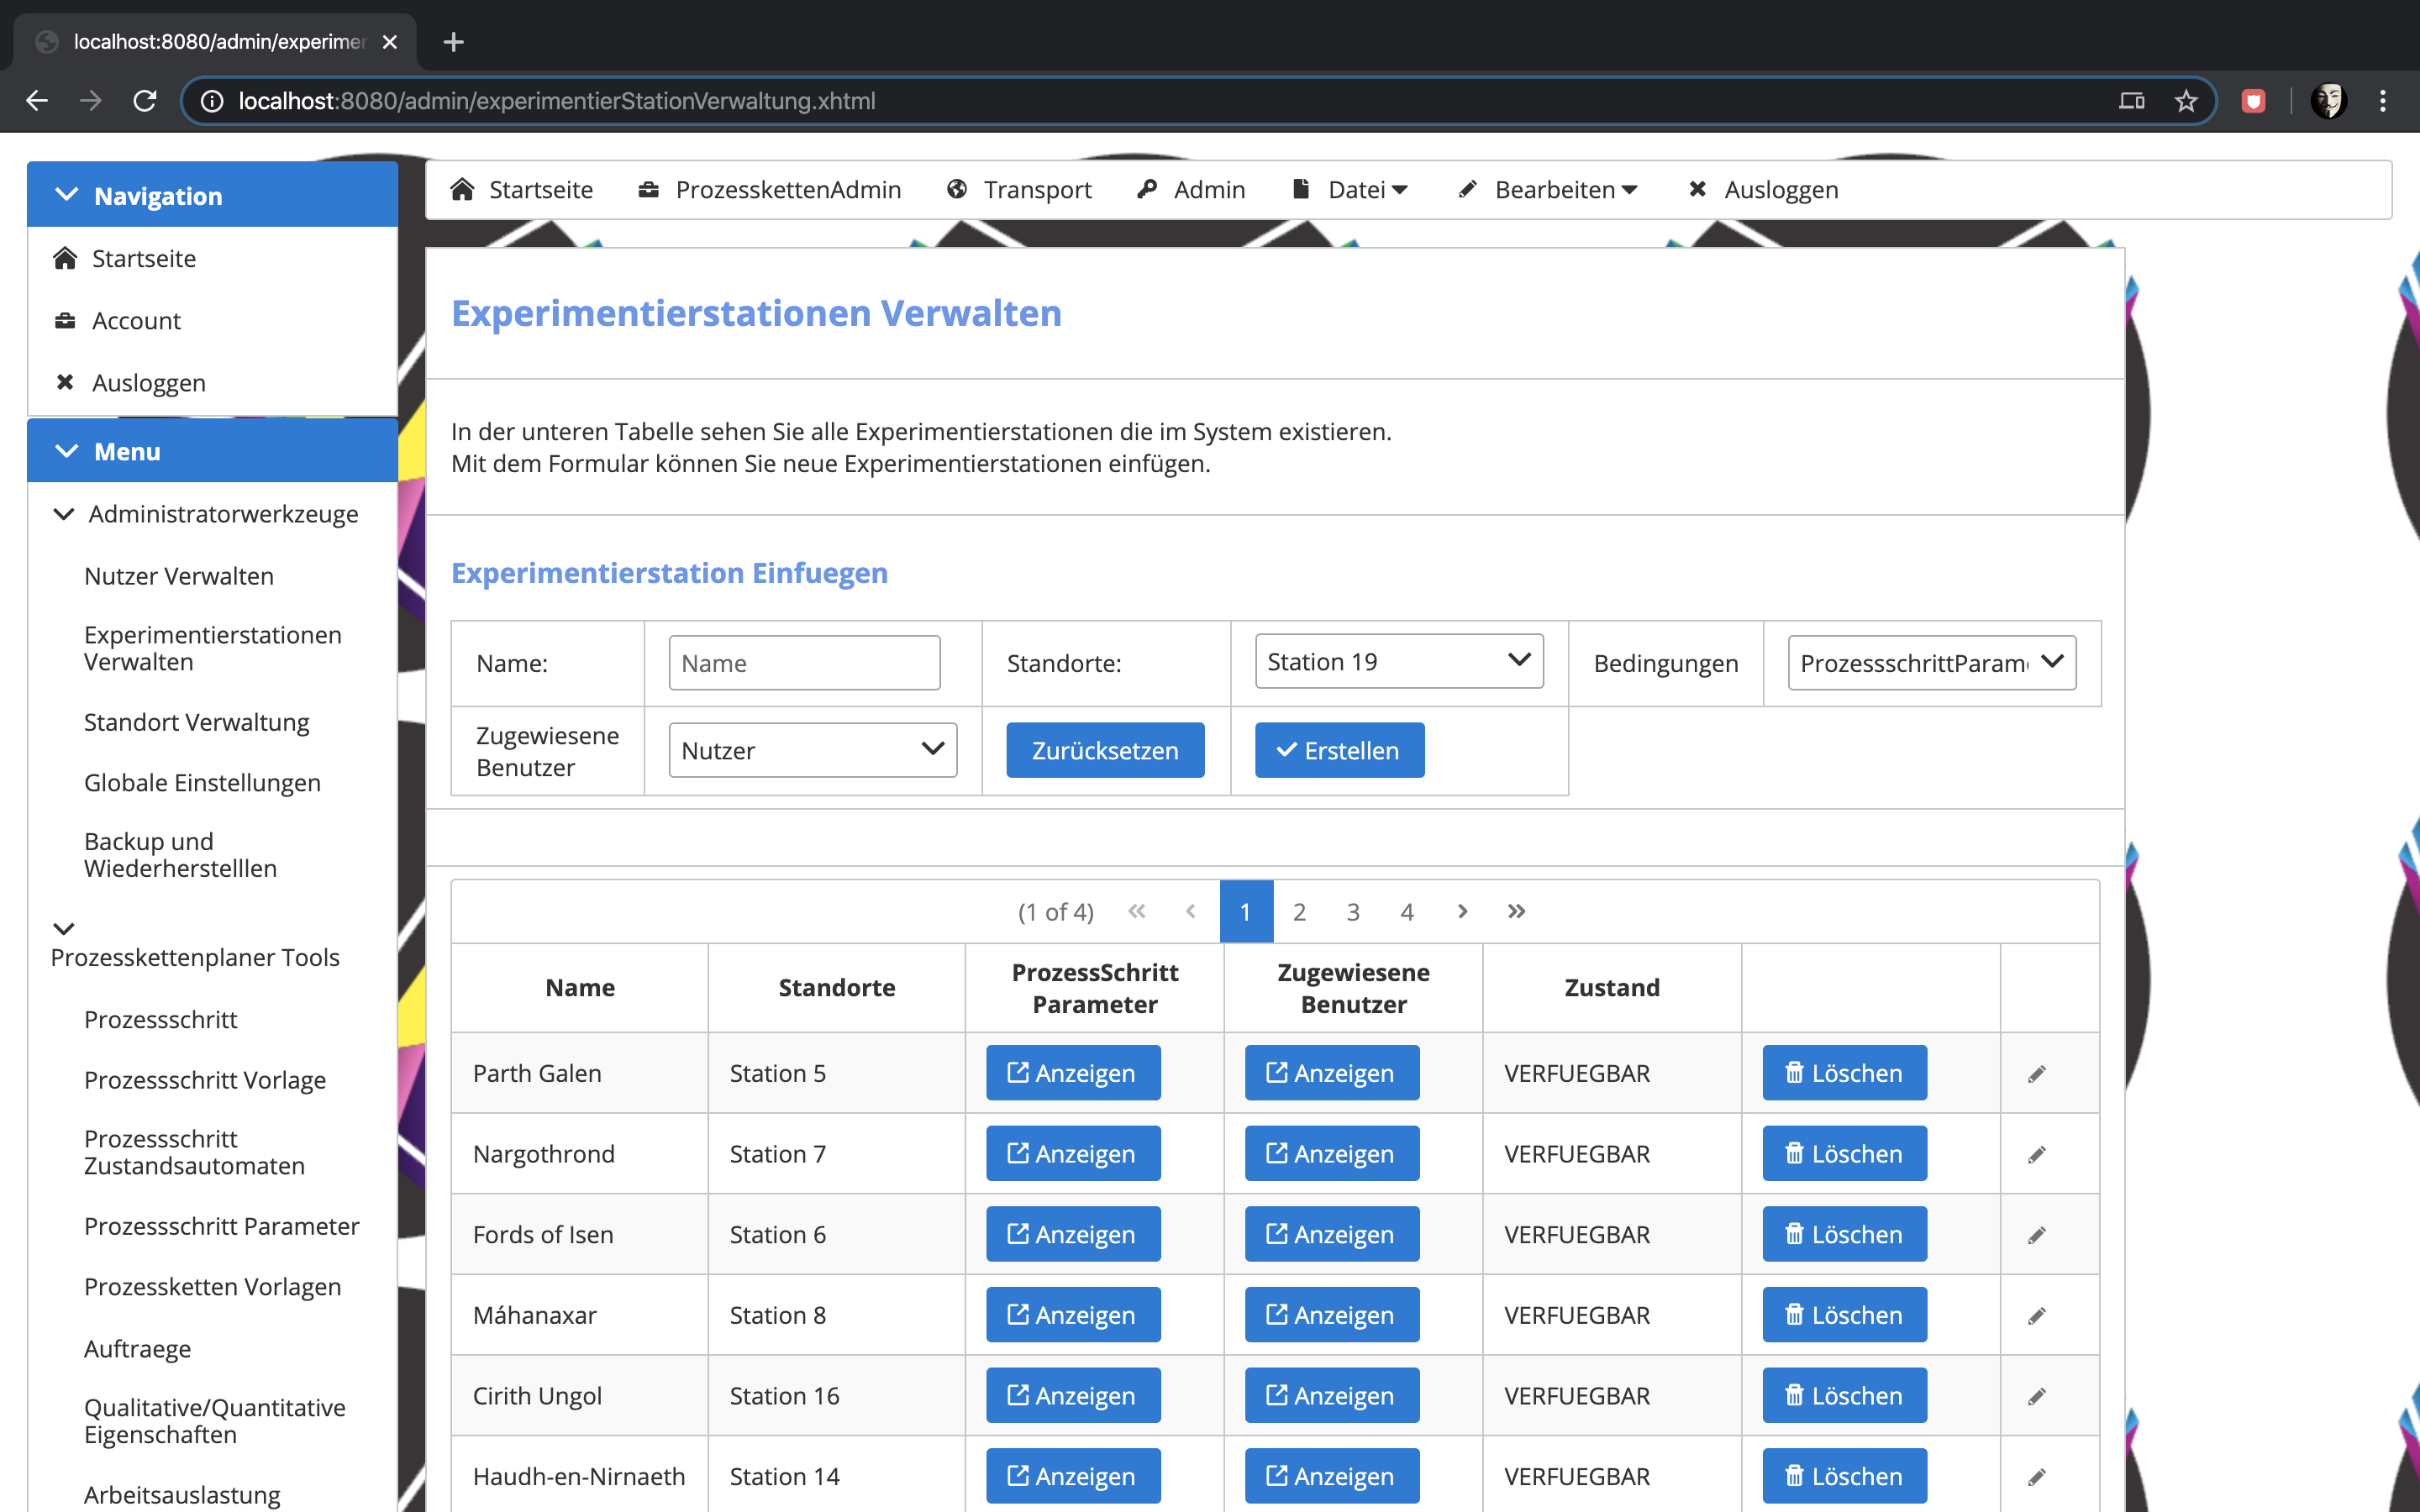
\includegraphics[width=1\textwidth]{Screenshots/3132.png}
\textit{Abbildung 3.1.3.2: Verwalten der Experimentierstationen}
} \\

\paragraph{Erstellen neuer Experimentierstationen:}

Für das Erstellen einer Experimentierstation benötigt man zwingend einen beliebigen Namen zum Eingeben, einen Standort, an dem die Experimentierstation erstellt wird und einen zugewiesenen Benutzer. Optional können Prozesschrittparameter als Bedingungen angegeben werden. \\

Nun befindet sich der Administrator auf der Seite zum \hyperlink{sc3.1.3.2}{Verwalten der Experimentierstationen}. Oben auf der Seite findet man eine \hyperlink{sc3.1.3.3}{Tabelle zum Einfügen von Experimentierstationen}. \\

\hypertarget{sc3.1.3.3}{
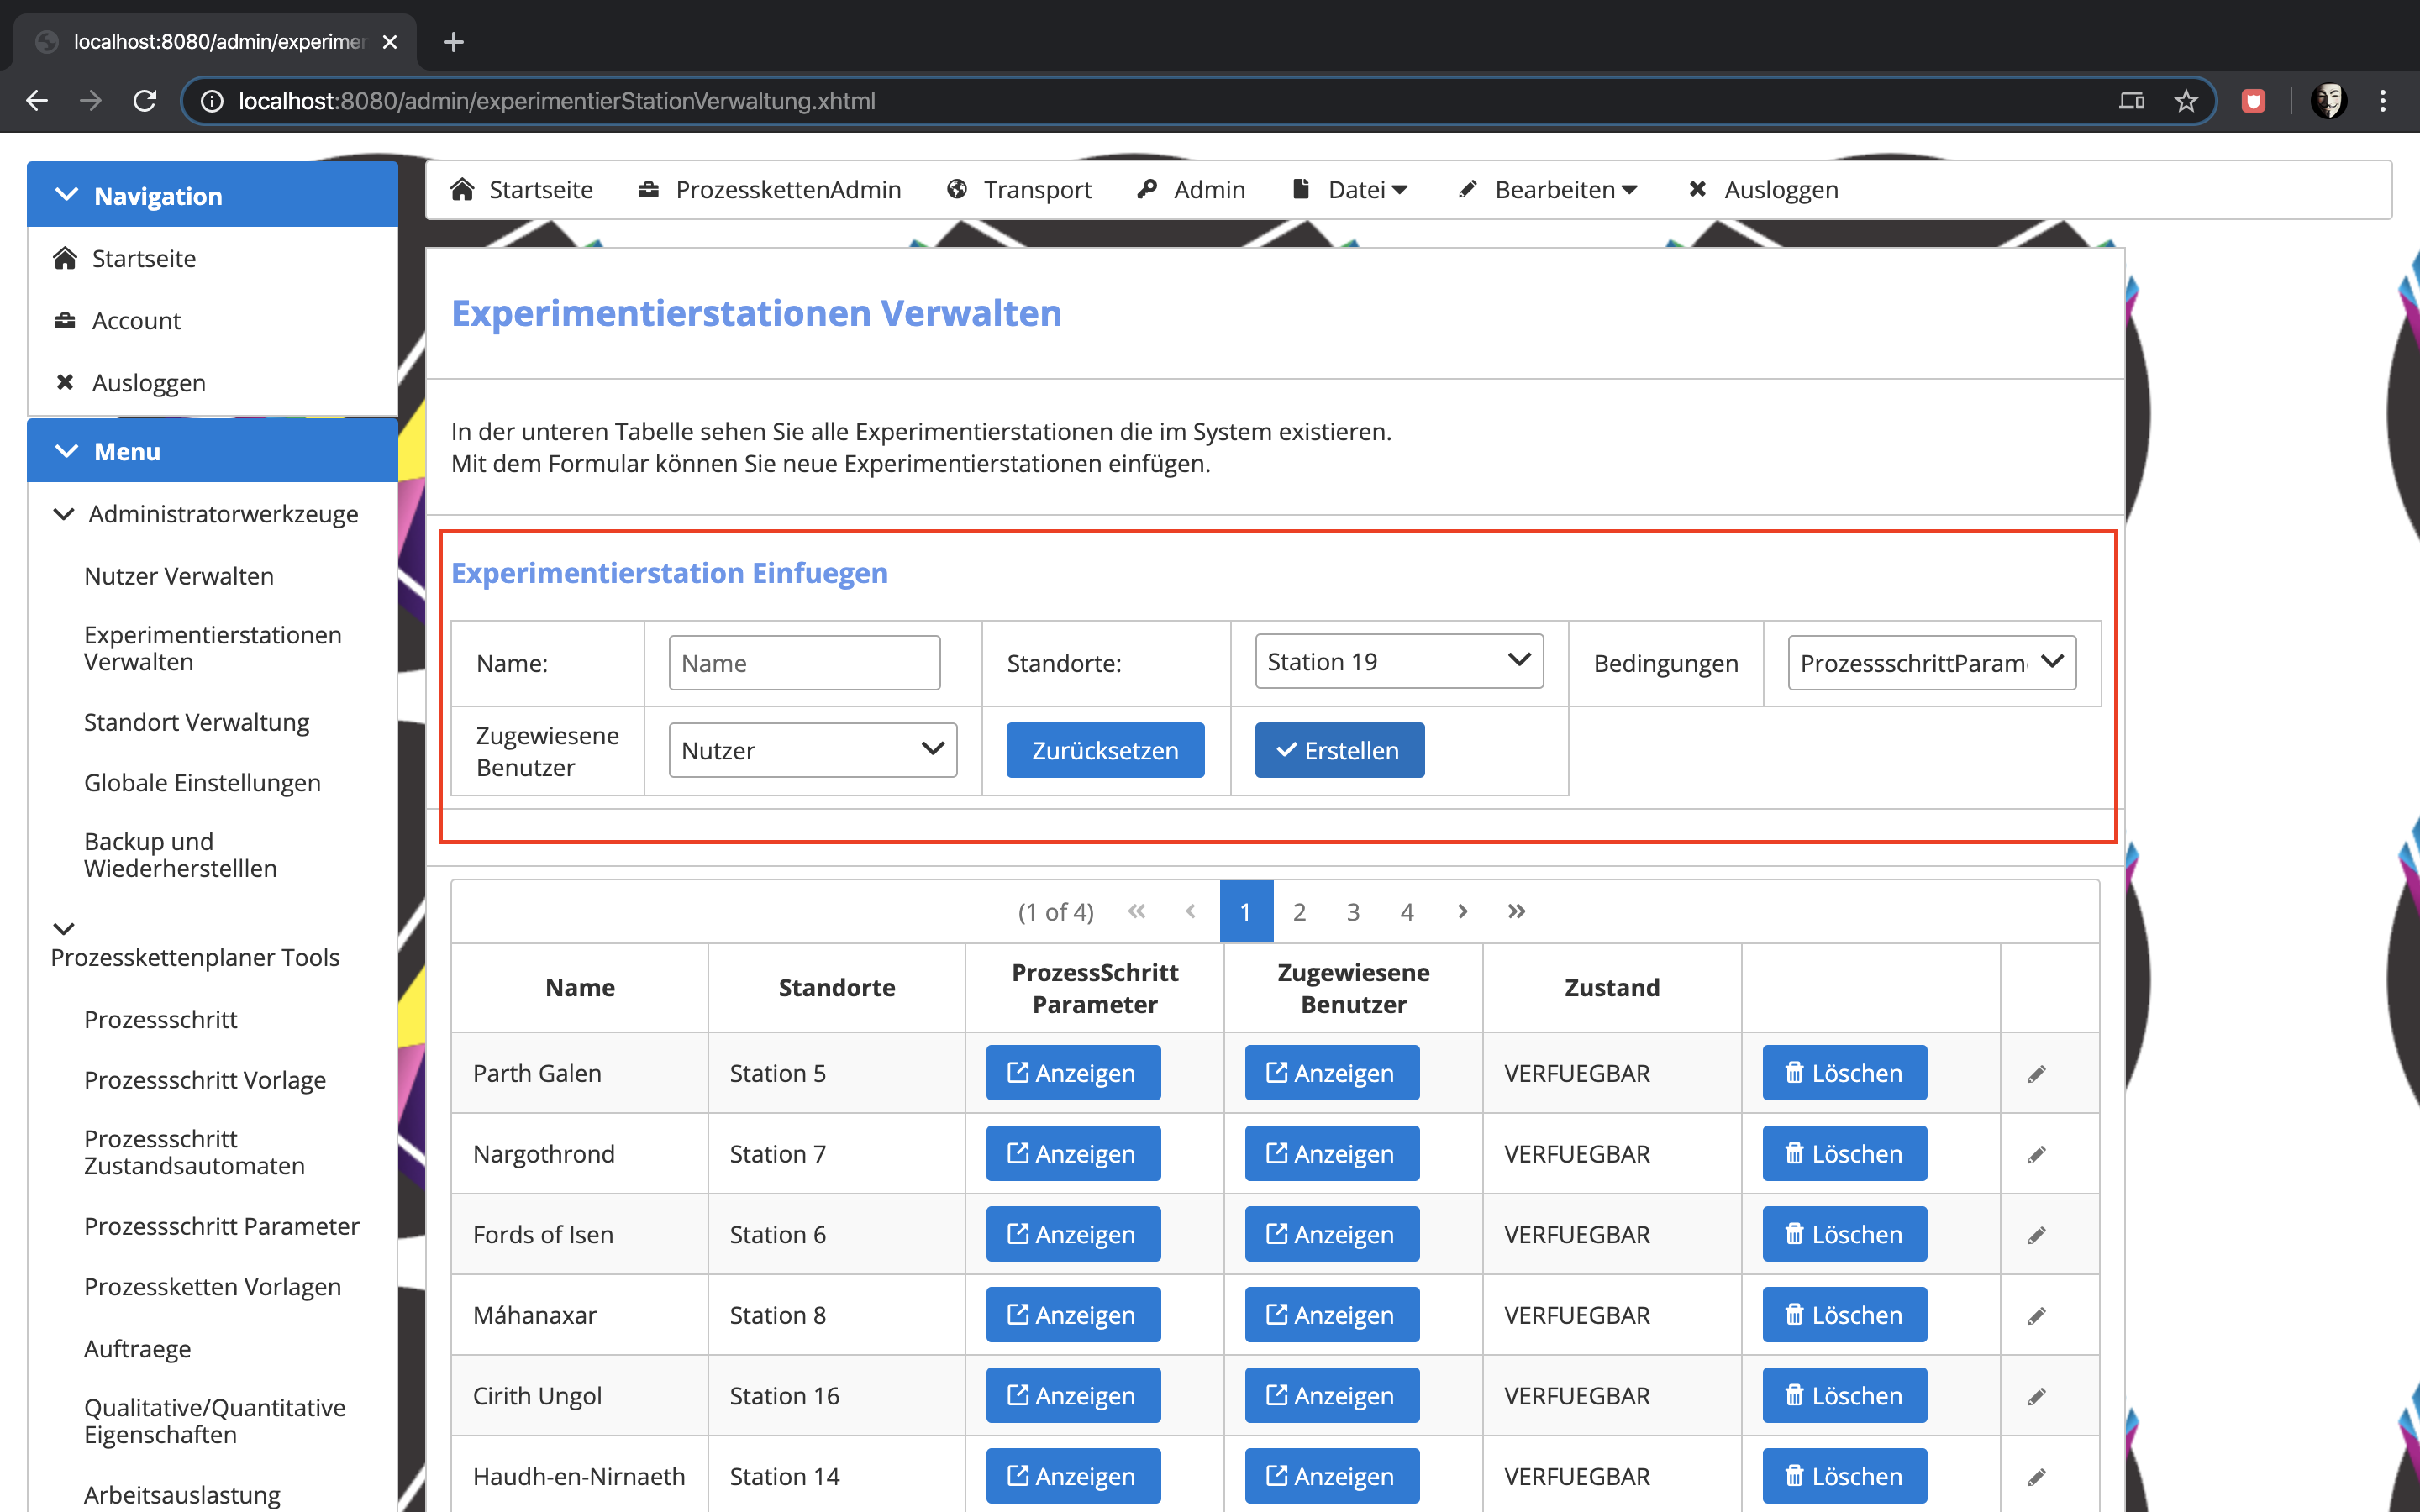
\includegraphics[width=1\textwidth]{Screenshots/3133.png}
\textit{Abbildung 3.1.3.3: Hinzufügen von Experimentierstationen}
} \\

Hier müssen ein beliebiger Name eingegeben und ein Nutzer und ein Standort ausgewählt werden. Dann kann man eine Experimentierstation erstellen. Optional können auch Prozesschrittparameter ausgewählt werden. In diesem Test werde ich alles in die Experimentierstation einfügen (\hyperlink{sc3.1.3.4}{Eingegebene Daten}). 

\hypertarget{sc3.1.3.4}{
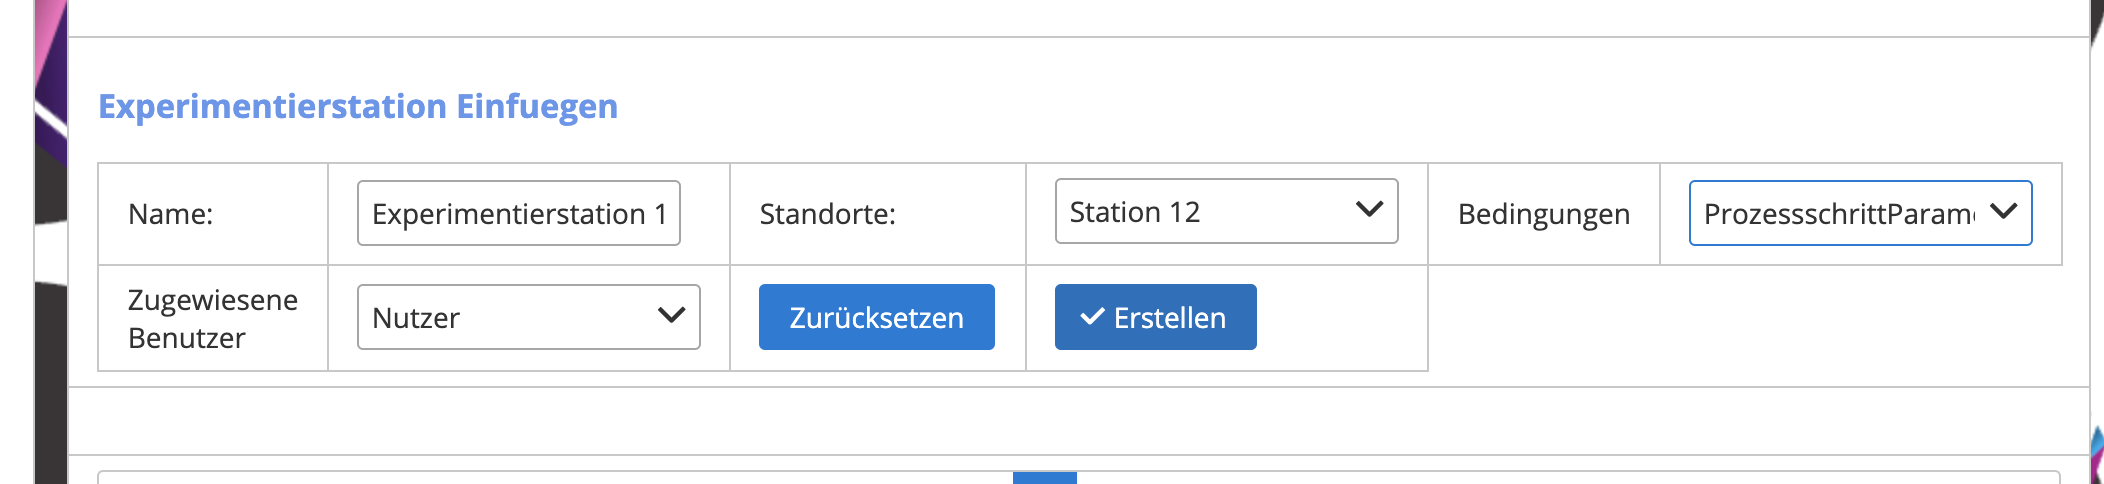
\includegraphics[width=1\textwidth]{Screenshots/3134.png}
\textit{Abbildung 3.1.3.4: Eingegebene Daten}
} \\

Es wurde der \textit{admin} als User zugewiesen und \textit{Sunfyre, Drogon, Meleys und Syrax} als Prozessschrittparameter hinzugefügt. \\

Nun überprüfe ich in der \hyperlink{sc3.1.3.5}{Tabelle}, ob die \textit{Experimentierstation 1} erstellt wurde. \\

\hypertarget{sc3.1.3.5}{
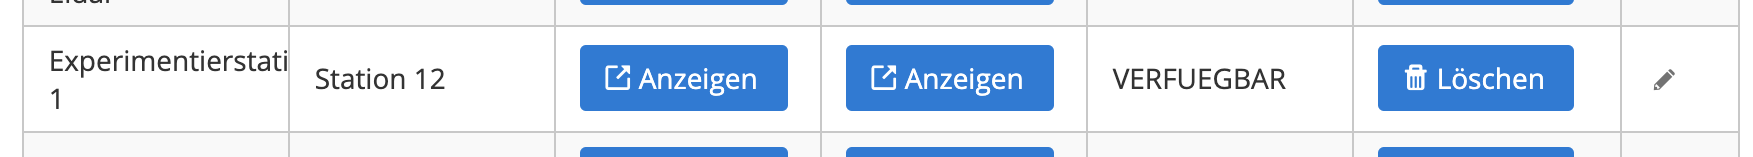
\includegraphics[width=1\textwidth]{Screenshots/3135.png}
\textit{Abbildung 3.1.3.5: Eben erstellte Daten in der Tabelle}
} \\

Wenn man in der Tabelle in der richtigen Zeile auf \hyperlink{sc3.1.3.6}{Anzeigen der Prozessschrittparameter} drückt, dann öffnet sich ein Menü, indem in einer Tabelle alle zugewiesenen Prozessparameter angezeigt werden. \\

\hypertarget{sc3.1.3.6}{
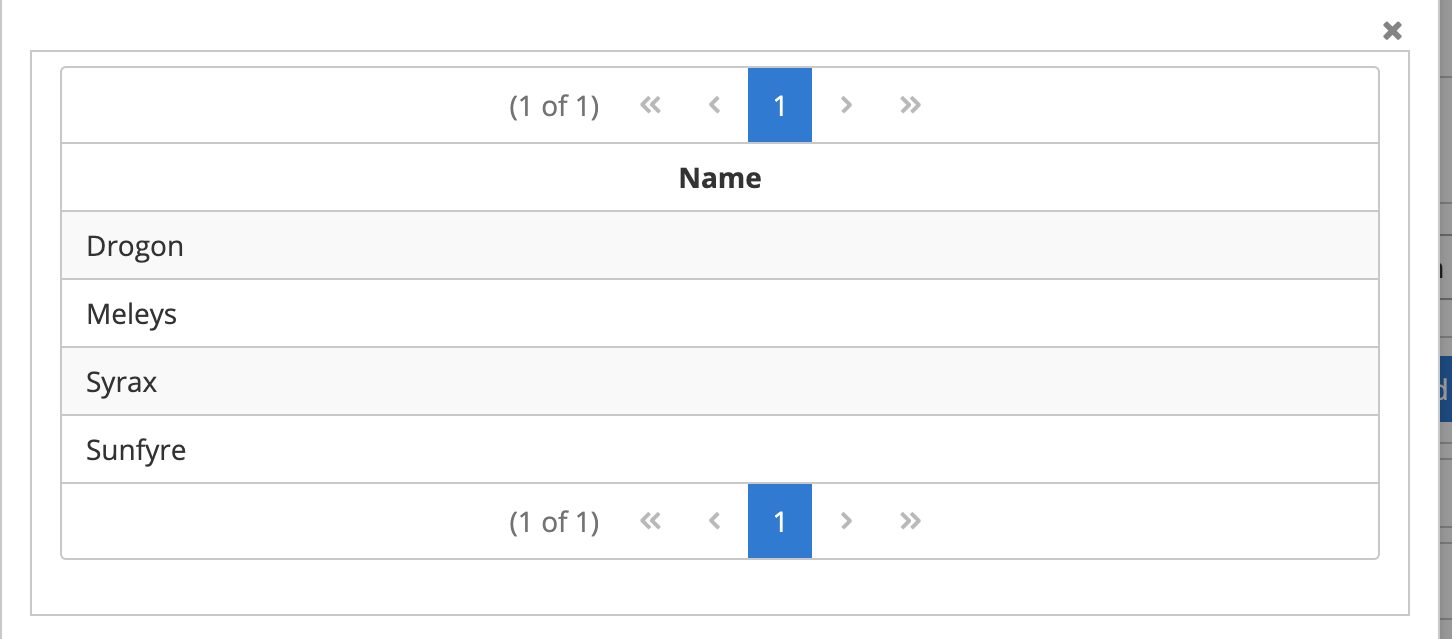
\includegraphics[width=1\textwidth]{Screenshots/3136.png}
\textit{Abbildung 3.1.3.6: Zugewiesene Prozessparameter}
} \\

Gleiches passiert wenn man \hyperlink{sc3.1.3.7}{Anzeigen der zugewiesenen Benutzer} drückt. 

\hypertarget{sc3.1.3.7}{
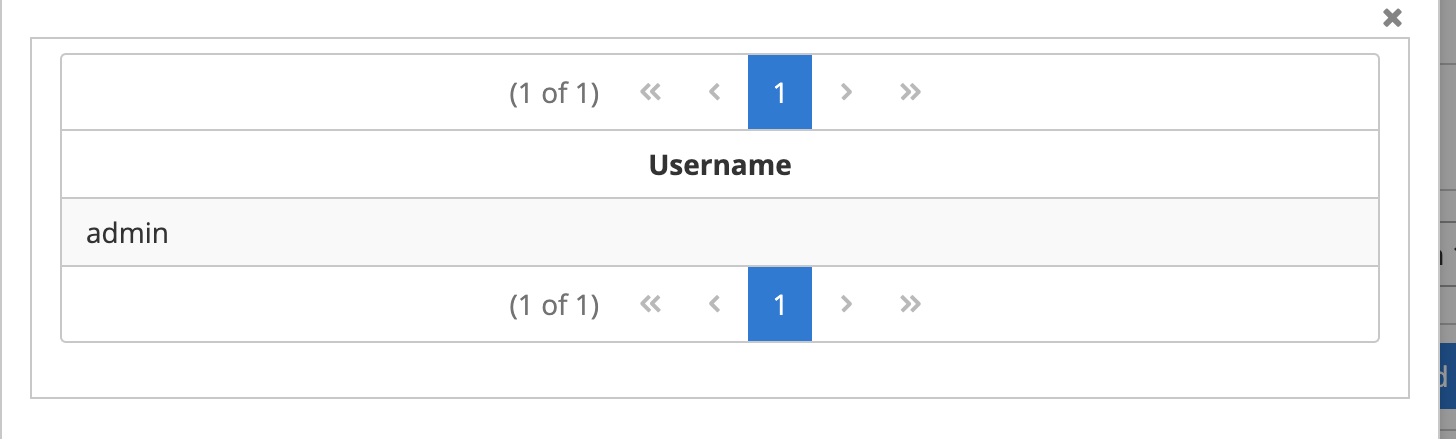
\includegraphics[width=1\textwidth]{Screenshots/3137.png}
\textit{Abbildung 3.1.3.7: Zugewiesene Benutzer}
} \\

Die Tests für das Hinzufügen und das Einsehen von Experimentierstationen verliefen erfolgreich. 

\paragraph{Bearbeiten von existierenden Experimentierstationen:} 


Die zu bearbeitende Experimentierstation heißt \hyperlink{sc3.1.3.8}{ES2}. Sie hat folgende \hyperlink{sc3.1.3.9}{Prozessschrittparameter} und \hyperlink{sc3.1.3.10}{Benutzer} zugewiesen\\

\hypertarget{sc3.1.3.8}{
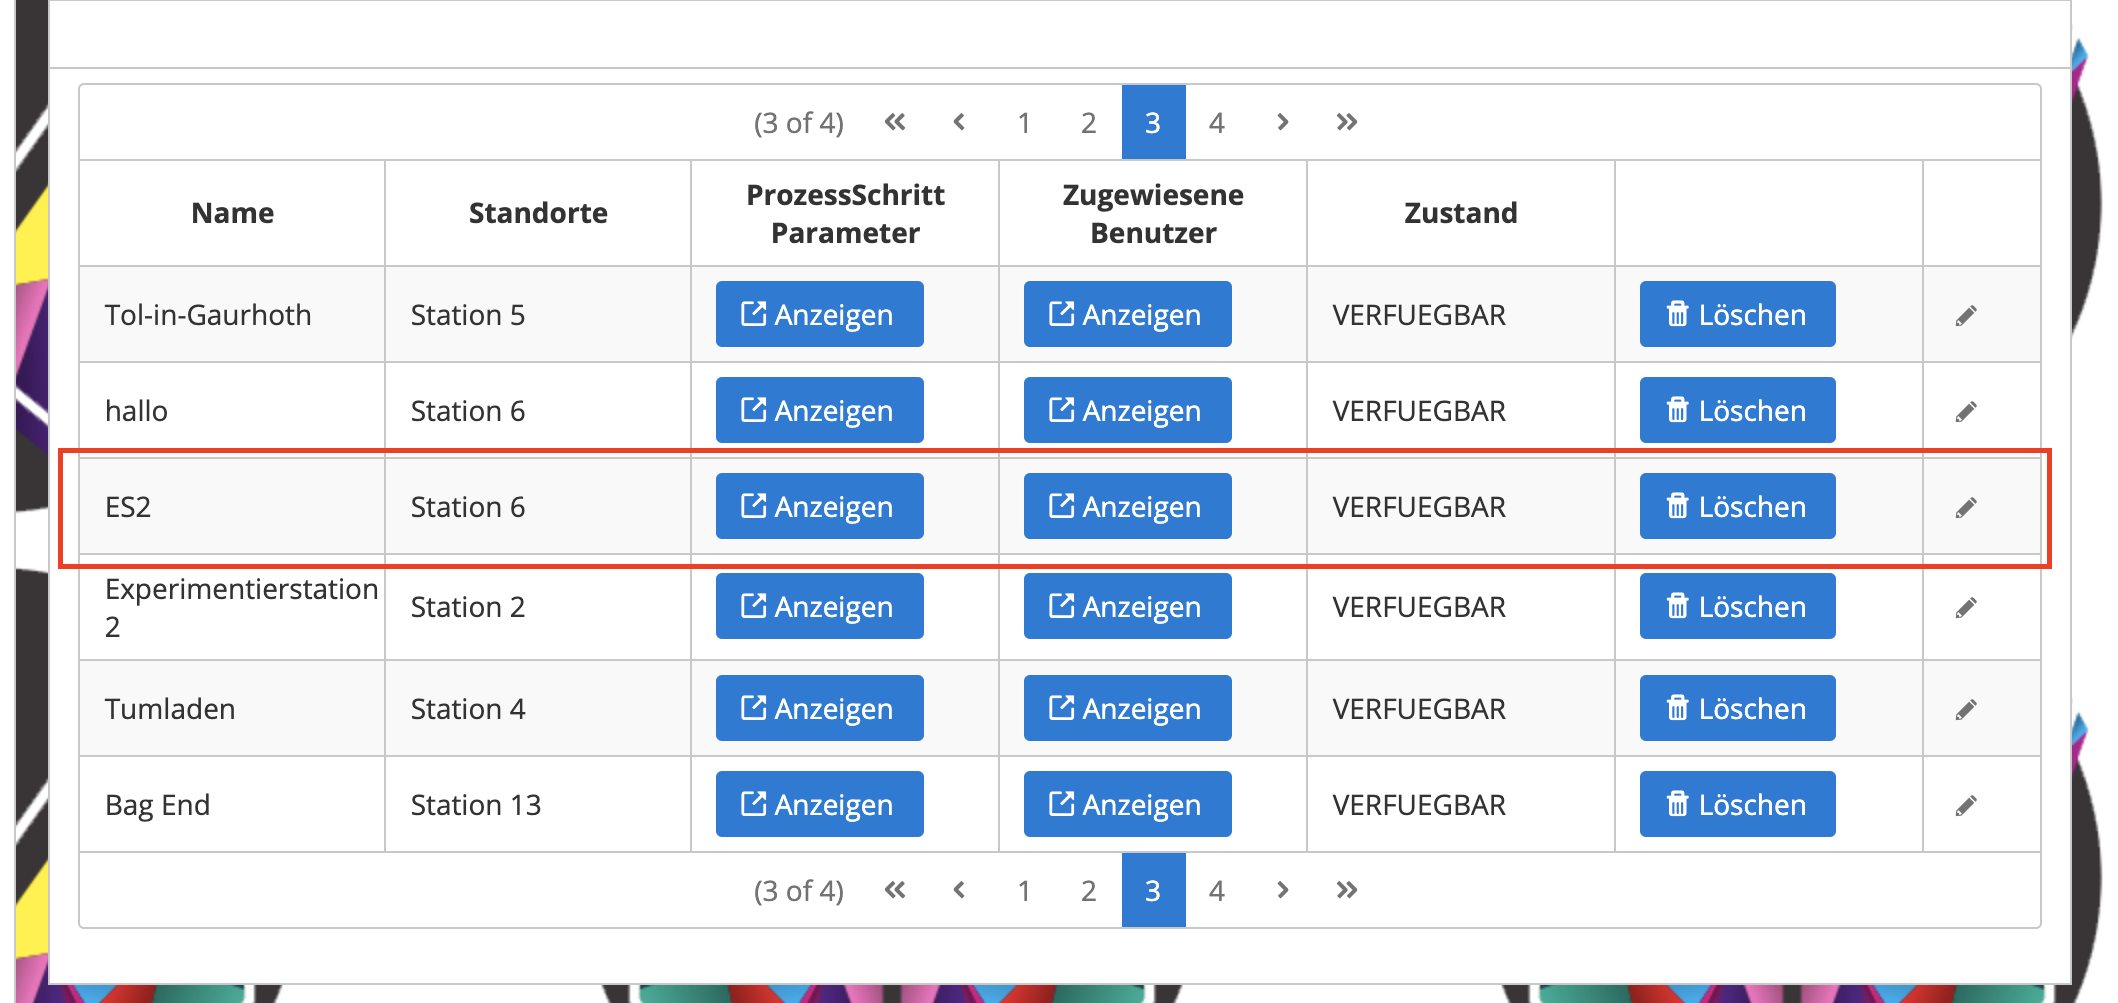
\includegraphics[width=1\textwidth]{Screenshots/3138.png}
\textit{Abbildung 3.1.3.8: Zu bearbeitende Experimentierstation}
} \\

\hypertarget{sc3.1.3.9}{
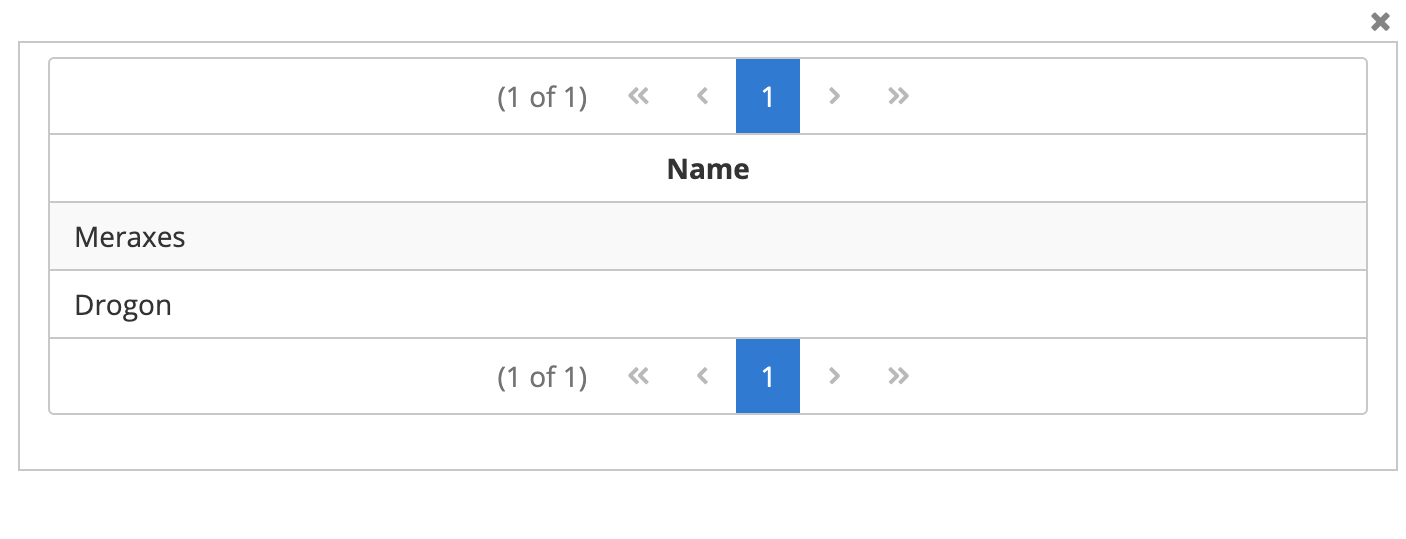
\includegraphics[width=1\textwidth]{Screenshots/3139.png}
\textit{Abbildung 3.1.3.9: Prozessschrittparameter der zu bearbeitende Experimentierstation}
} \\

\hypertarget{sc3.1.3.10}{
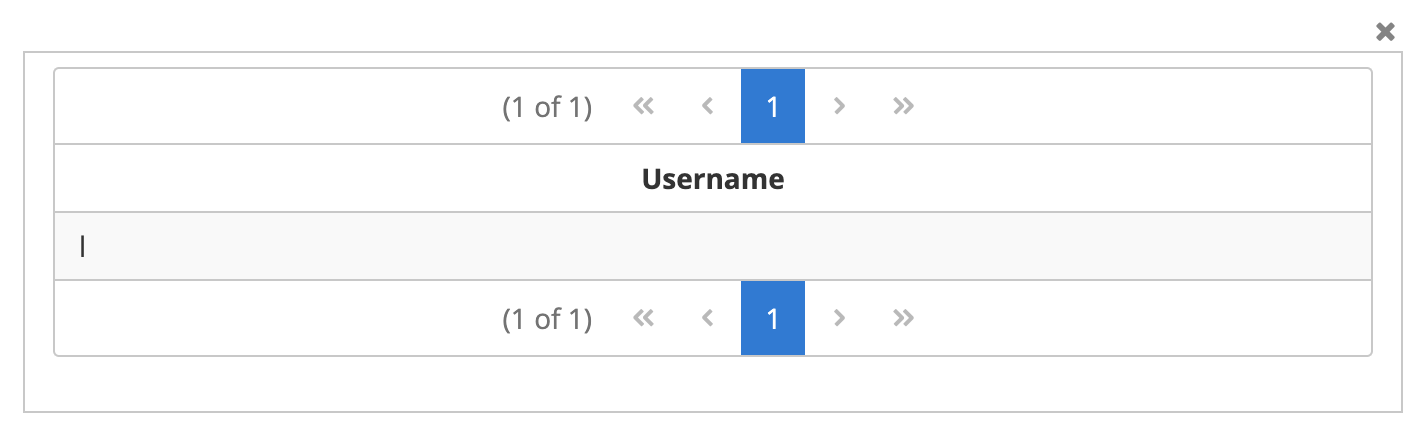
\includegraphics[width=1\textwidth]{Screenshots/31310.png}
\textit{Abbildung 3.1.3.10: Benutzer der zu bearbeitende Experimentierstation}
} \\

Jetzt wollen wir den Benutzer \textit{l} entfernen und den Benutzer \textit{t} hinzufügen. Hierfür gehen wir in der Zeile von ES2 auf den  \hyperlink{sc3.1.3.11}{Stift zum Bearbeiten} und öffnen das Ausklappfenster in der Spalte der zugewiesenen Benutzer. Hier wählen wir den neuen Benutzer aus und drücken rechts auf den Haken um zu speichern. \\

\hypertarget{sc3.1.3.11}{
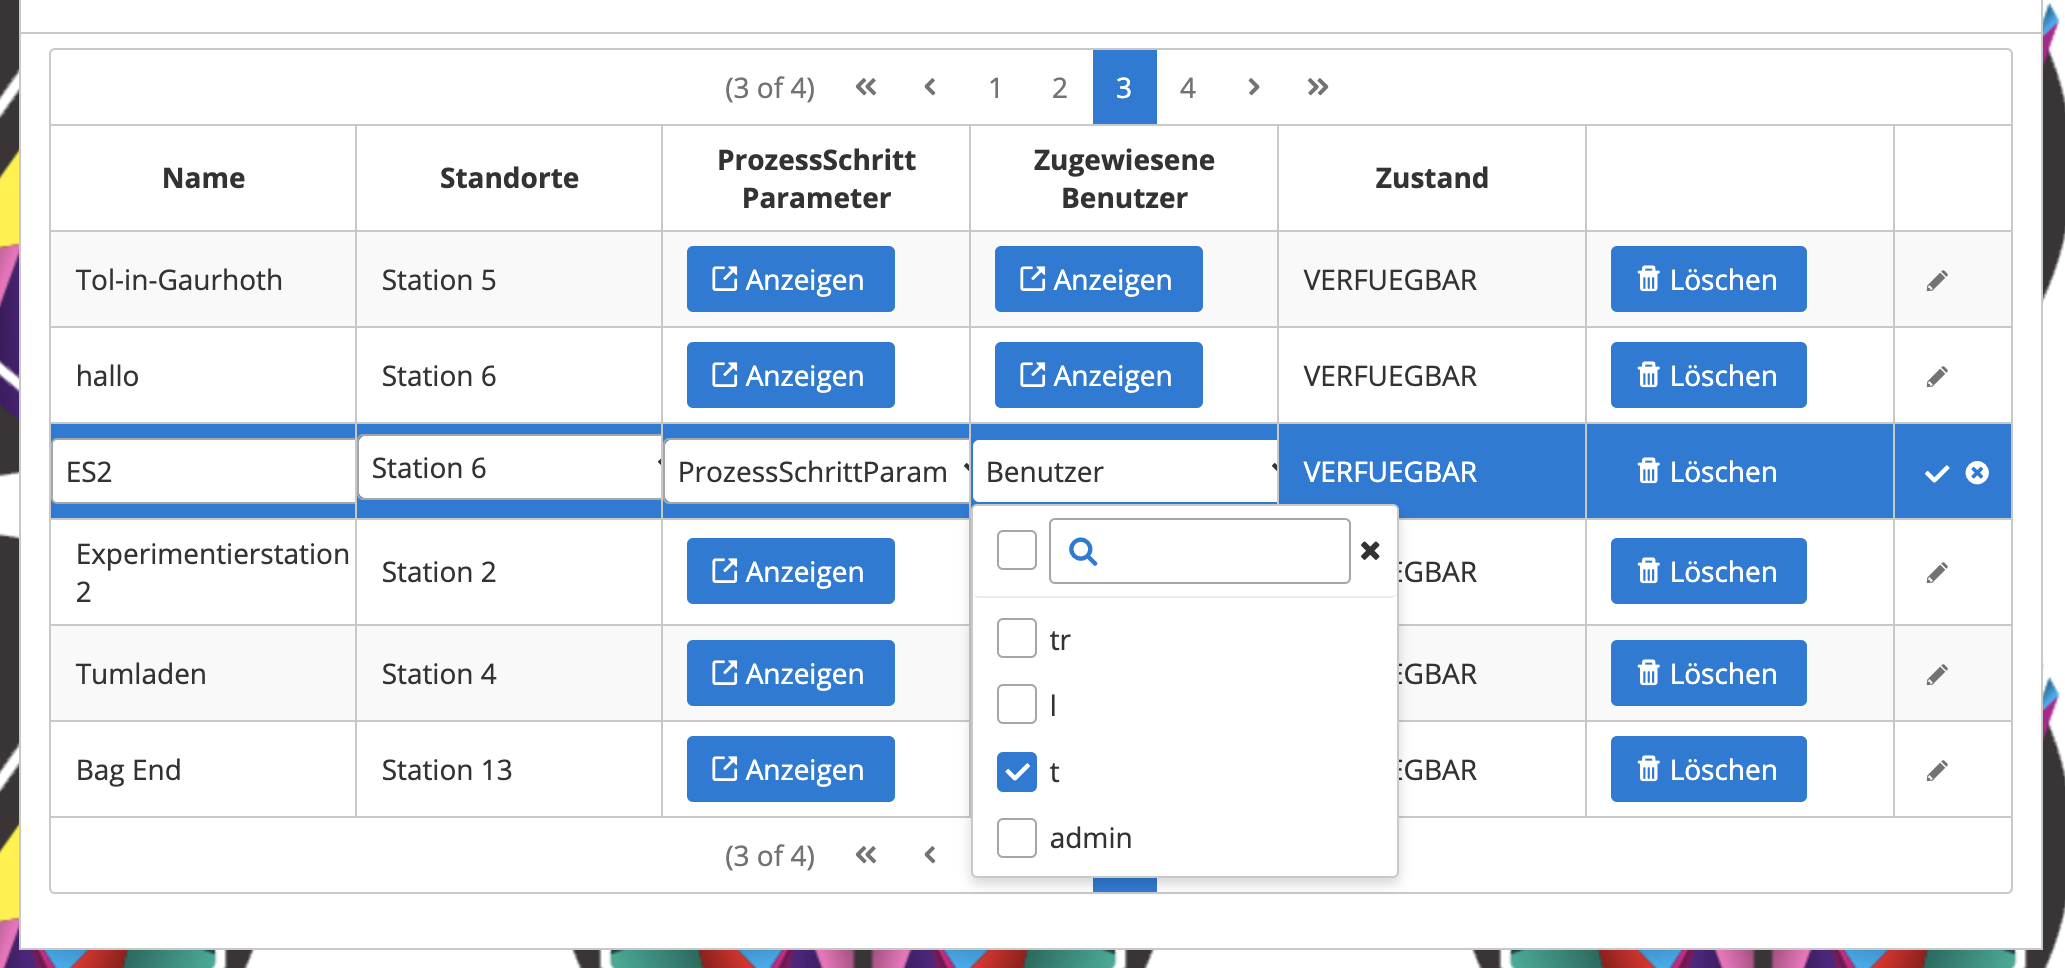
\includegraphics[width=1\textwidth]{Screenshots/31311.png}
\textit{Abbildung 3.1.3.11: Benutzer bearbeiten}
} \\

Anschließend sieht man in der \hyperlink{sc3.1.3.12}{Tabelle} in dem \textit{Anzeigen}-Menü, dass der Benutzer gewechselt wurde.\\

\hypertarget{sc3.1.3.12}{
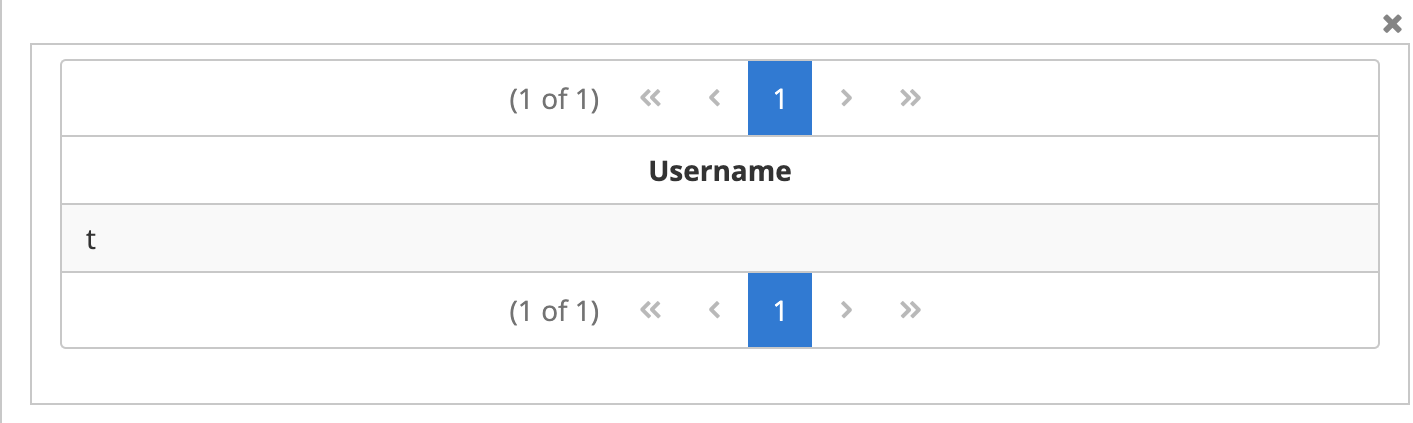
\includegraphics[width=1\textwidth]{Screenshots/31312.png}
\textit{Abbildung 3.1.3.12: Benutzer bearteitet}
} \\

Der Test verlief erfolgreich. die Tests für das bearbeiten von Name, Standort und Prozessschrittparameter wurde analog zu diesem getestet und waren ebenfalls erfolgreich.

\paragraph{Löschen von Experimentierstationen:}


Nun werde ich die Experimentierstation mit dem Namen \textit{Experimentierstation 2} löschen. Hierzu gehe ich in der Tabelle in der entsprechenden Zeile auf  \hyperlink{sc3.1.3.13}{löschen}, und die Experimentierstation wird gelöscht.\\

\hypertarget{sc3.1.3.13}{
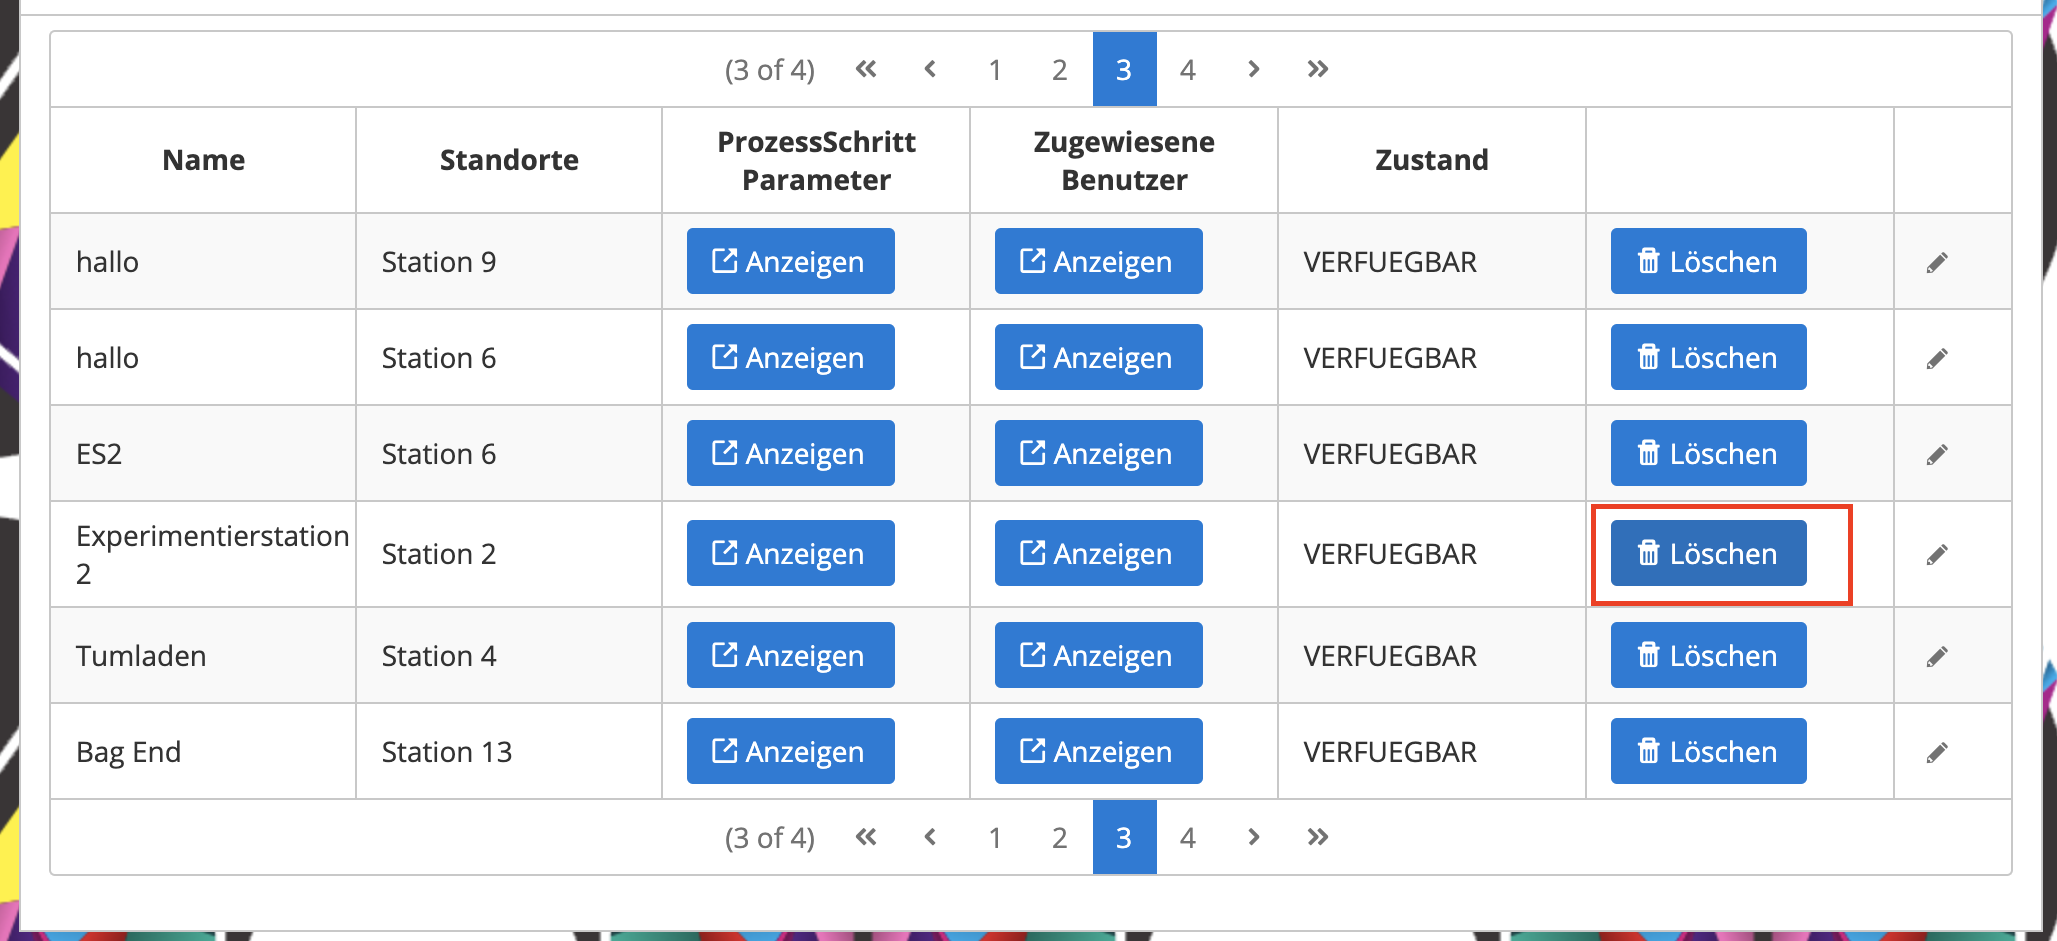
\includegraphics[width=1\textwidth]{Screenshots/31313.png}
\textit{Abbildung 3.1.3.13: Experimentierstation löschen}
} \\

\hypertarget{sc3.1.3.14}{
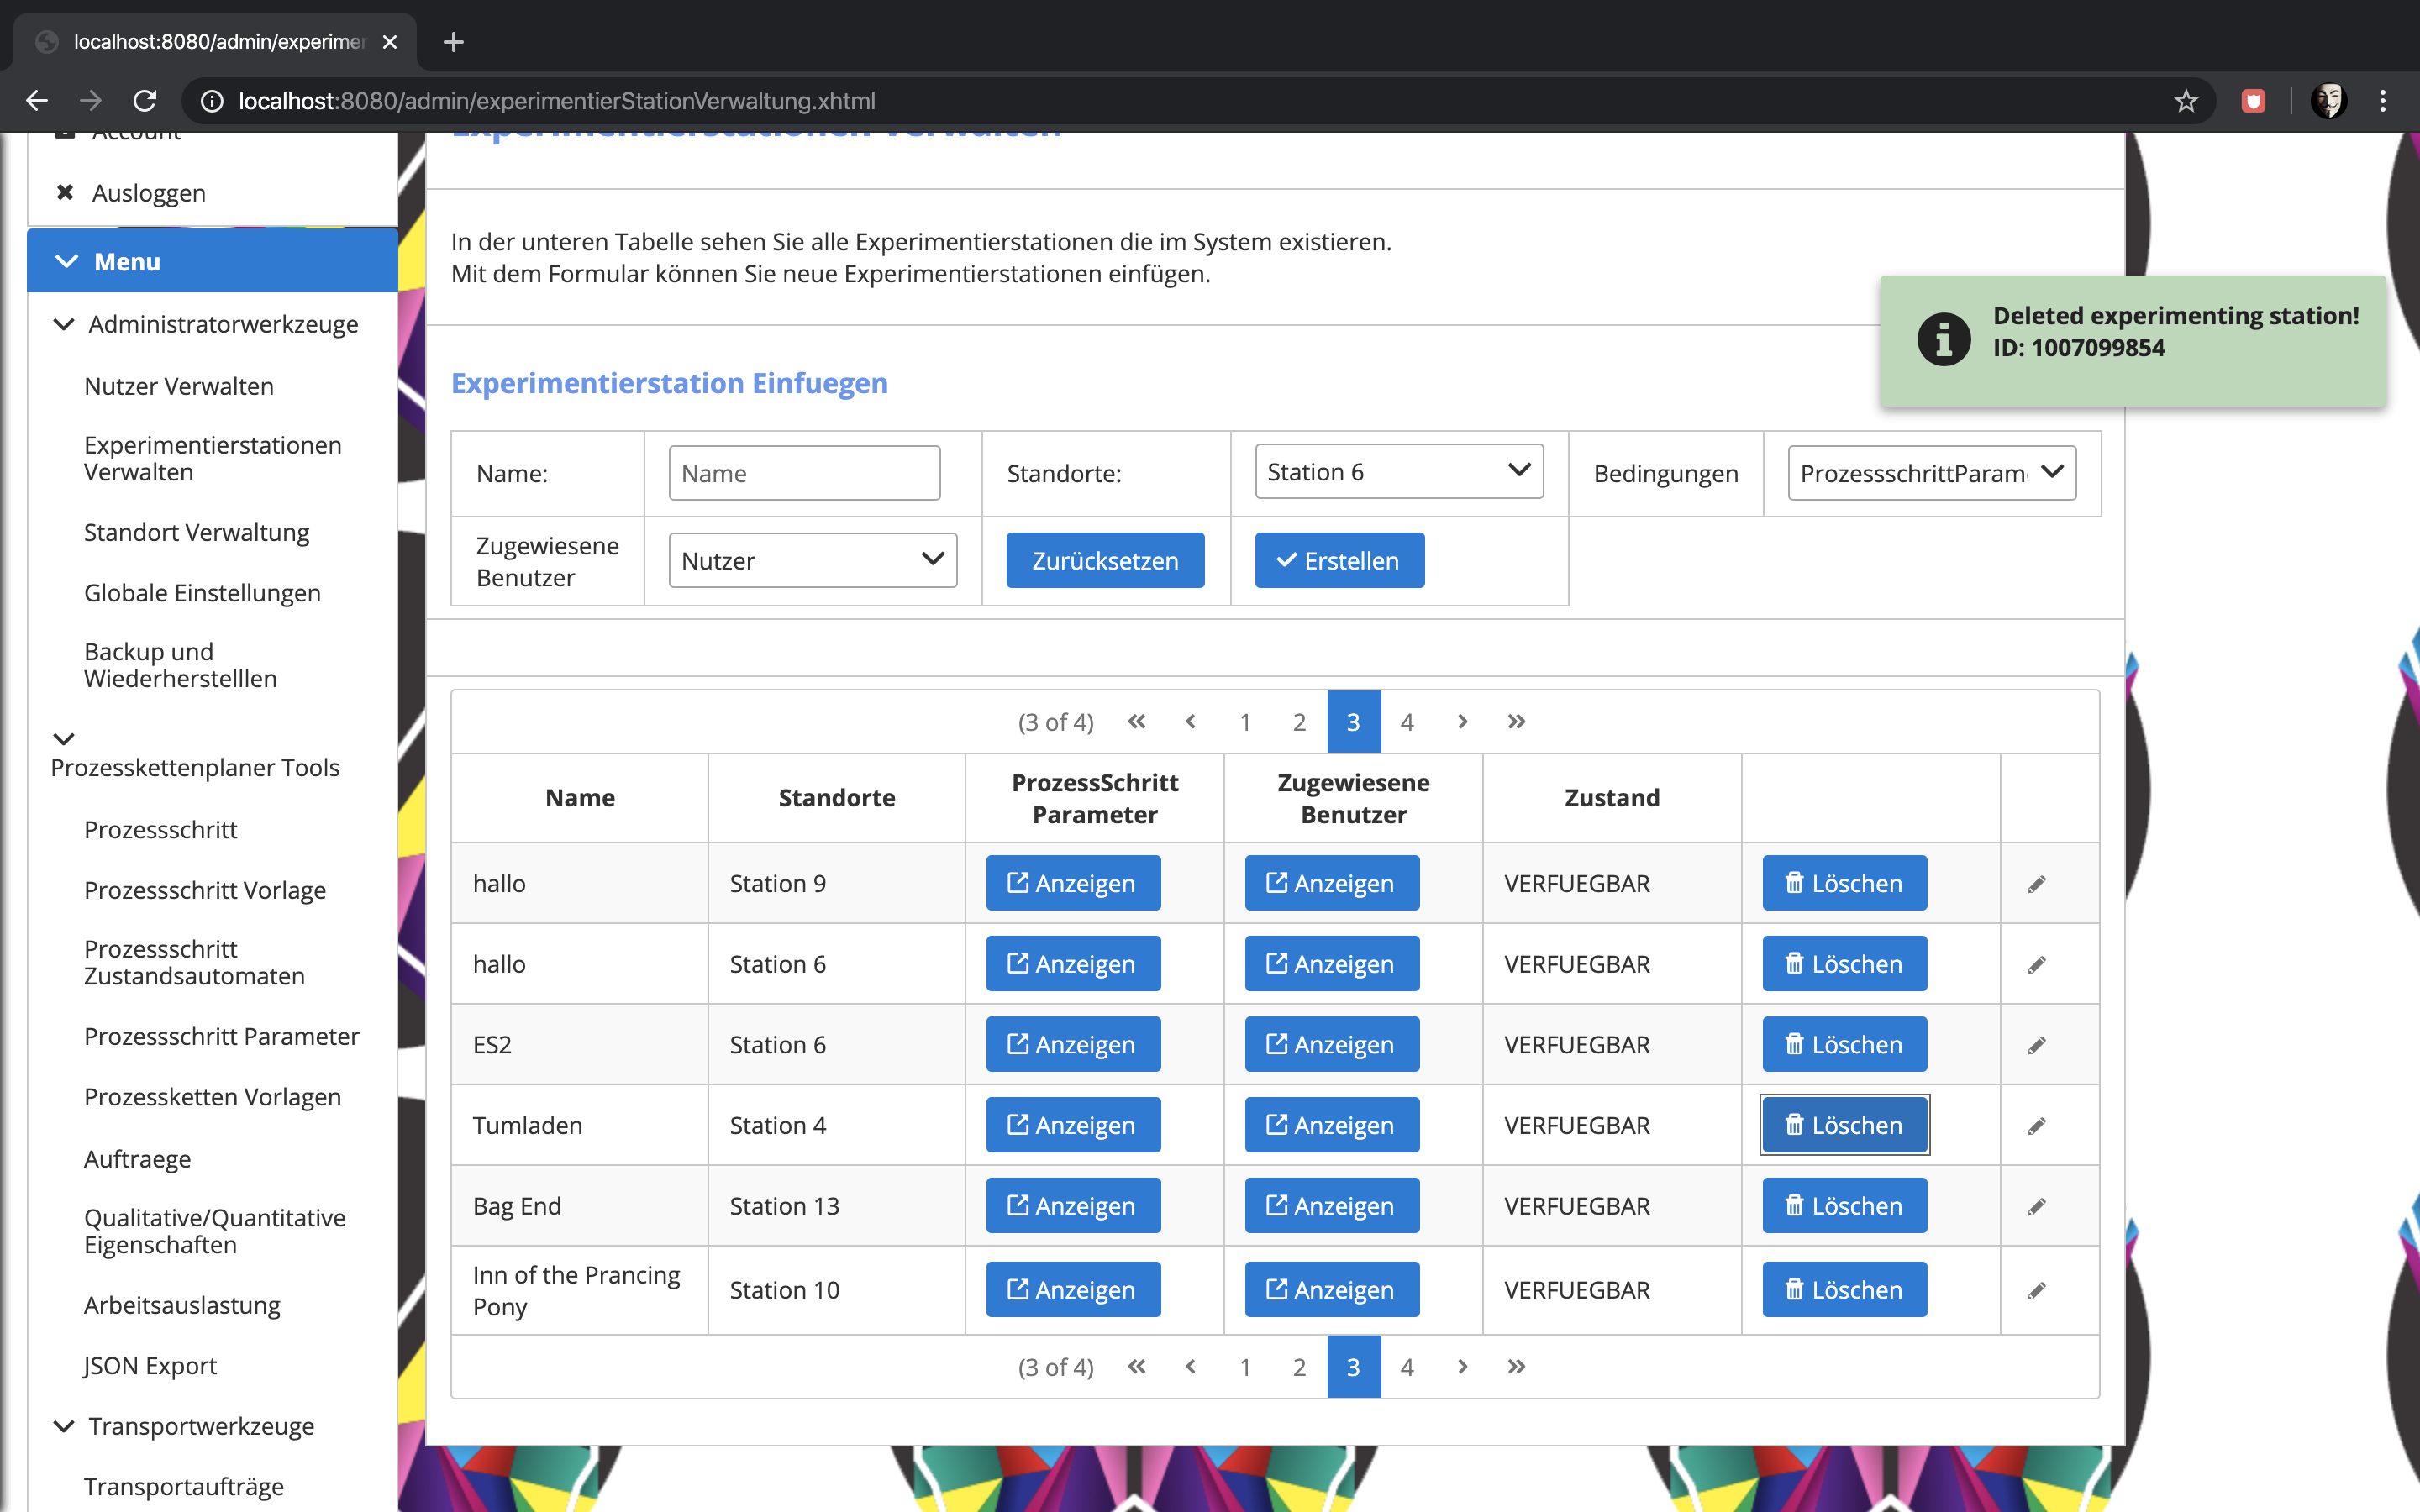
\includegraphics[width=1\textwidth]{Screenshots/31314.png}
\textit{Abbildung 3.1.3.14: Experimentierstation gelöscht}
} \\

\hyperlink{sc3.1.3.14}{Hier} sieht man eine Löschbestätigung oben rechts in der Ecke und der Eintrag wurde aus der Tabelle gelöscht. Auch nach einem erneuten Laden der Seite bleibt sie gelöscht. Also ist auch dieser Test erfolgreich. 

%%

\subsubsection{Anwendungsfall: Standort Test per Hand}

Der Administrator kann über ein Formular mit dem Standort auf der entsprechenden Website interagieren. Auf der entsprechenden Website kann der Benutzer den Standort anzeigen, ändern und löschen.\\

\hypertarget{sc3.1.4.1}{
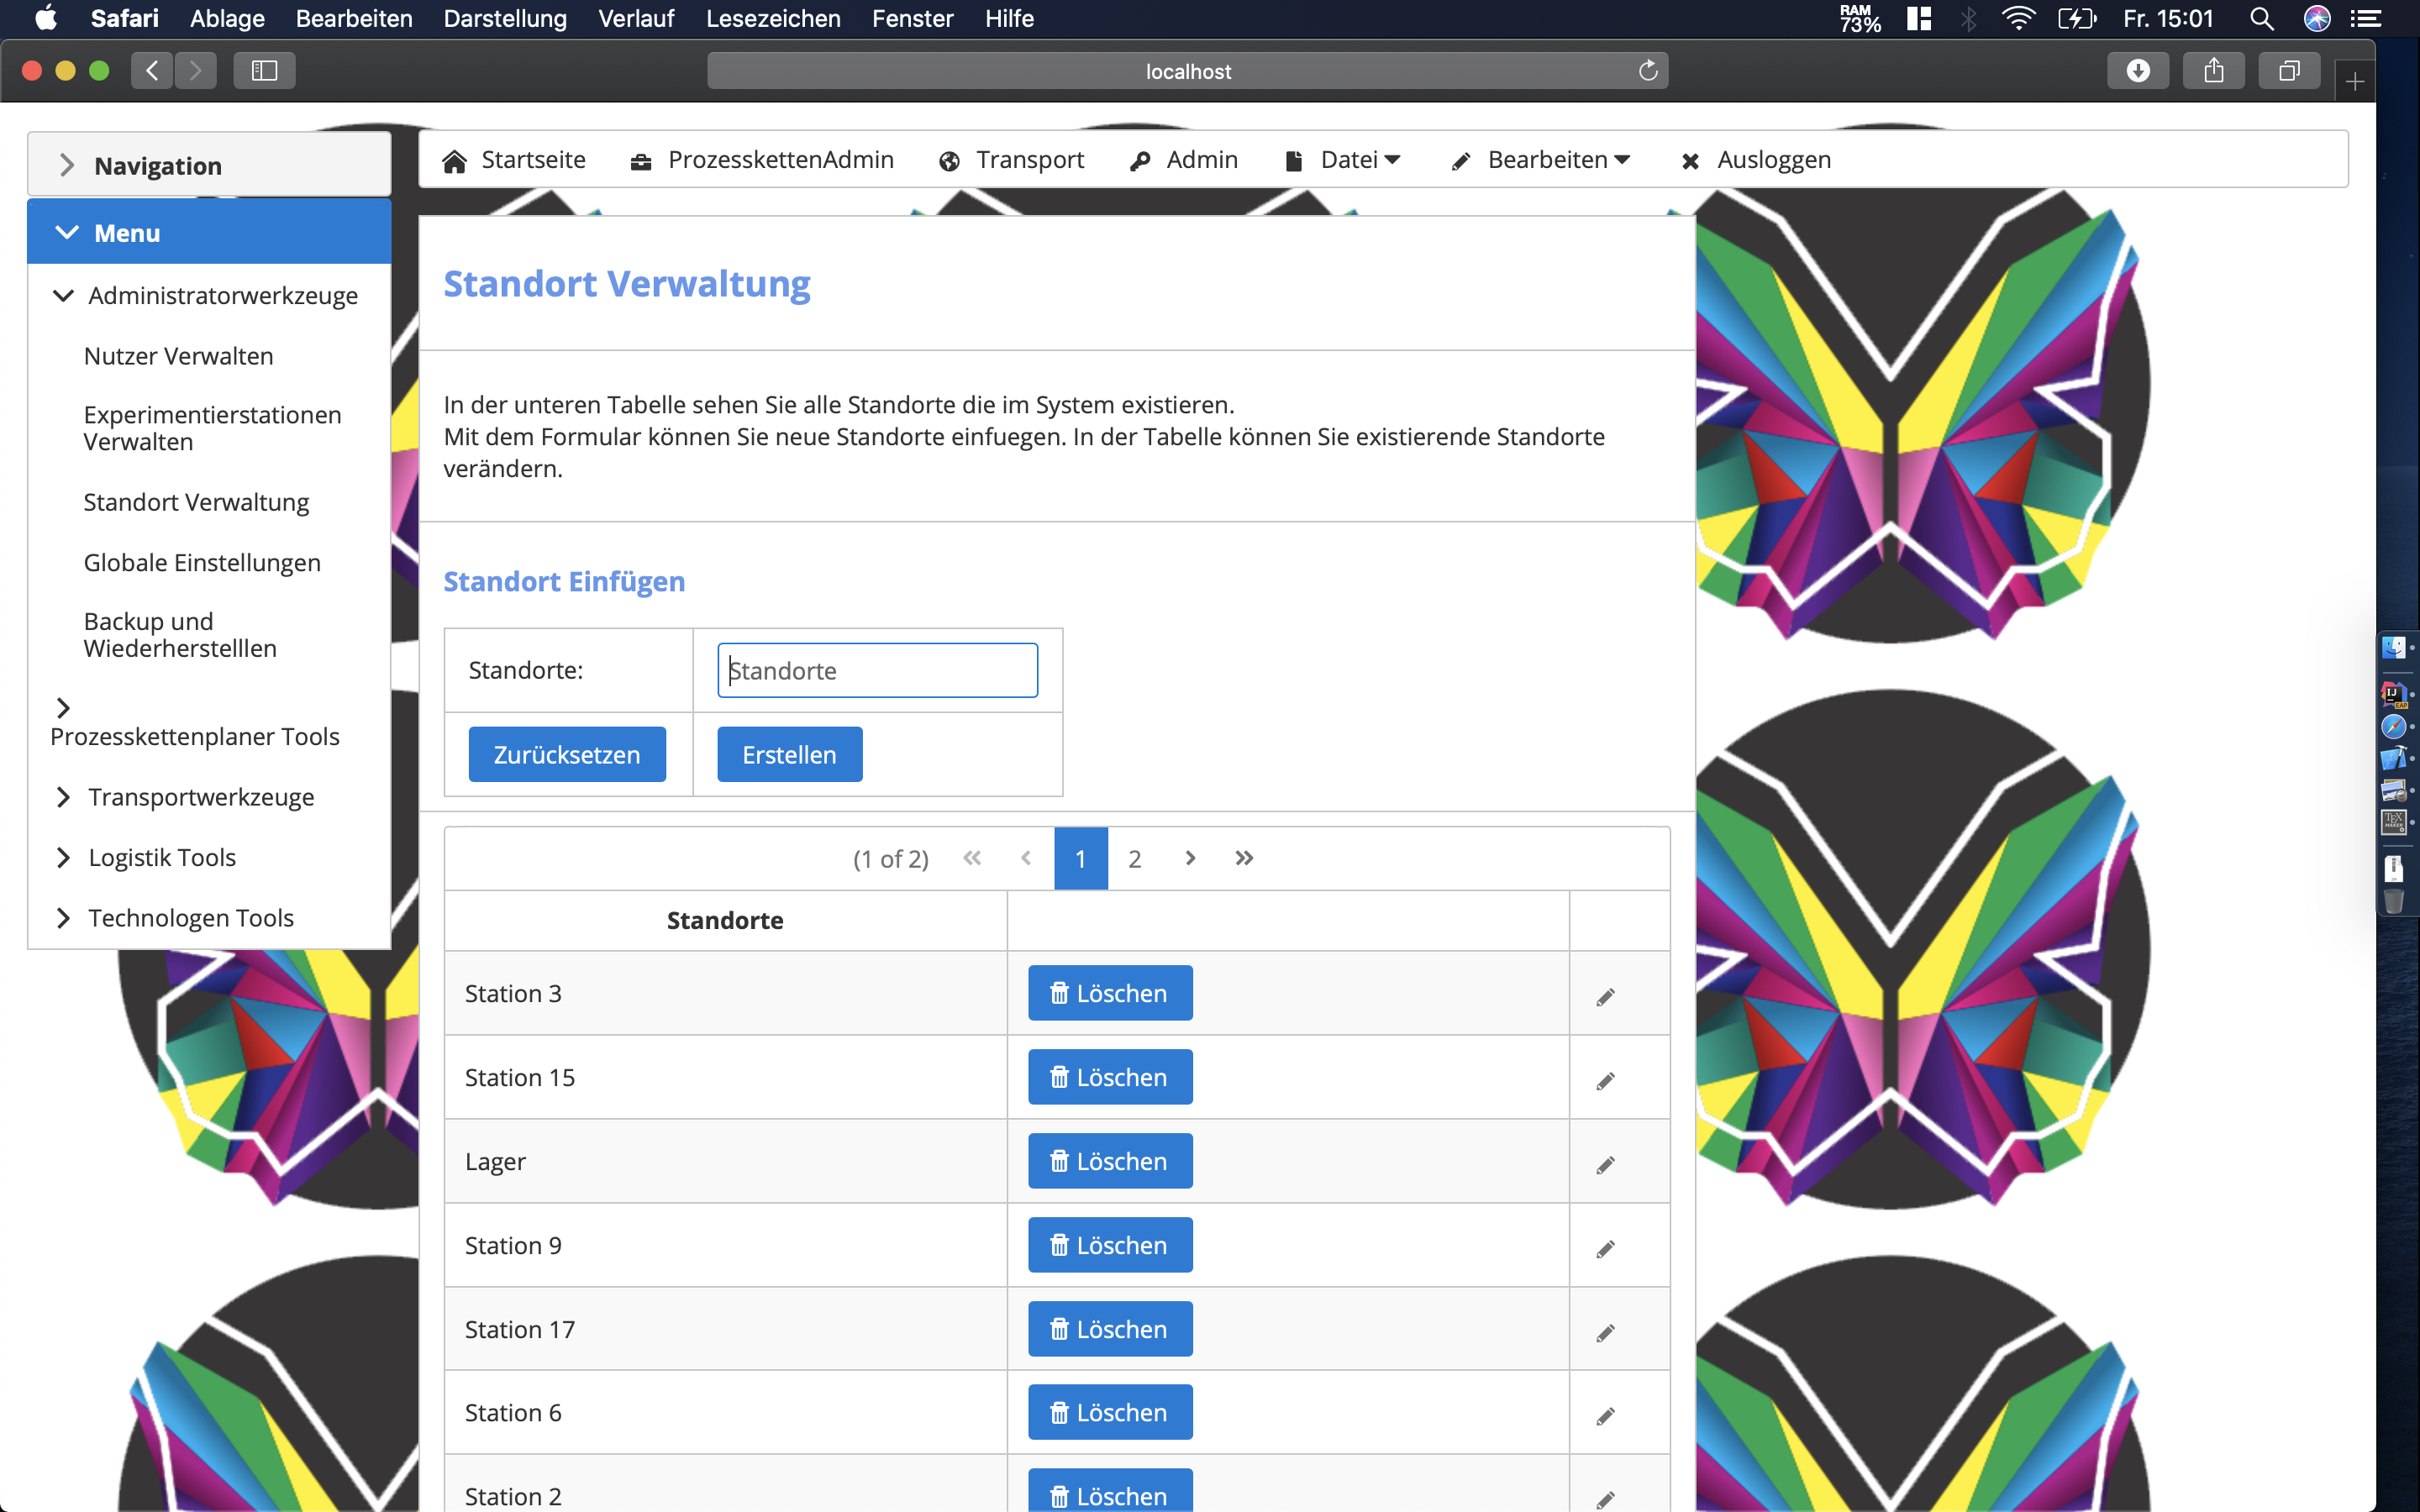
\includegraphics[width=1\textwidth]{Screenshots/4StandOrtFormular.png}
\textit{Abbildung 3.1.4.1: Standort Formular}
} \\

Wenn ein Standort erstellt wird, wird eine Bestätigungsnachricht empfangen.\\

\hypertarget{sc3.1.4.2}{
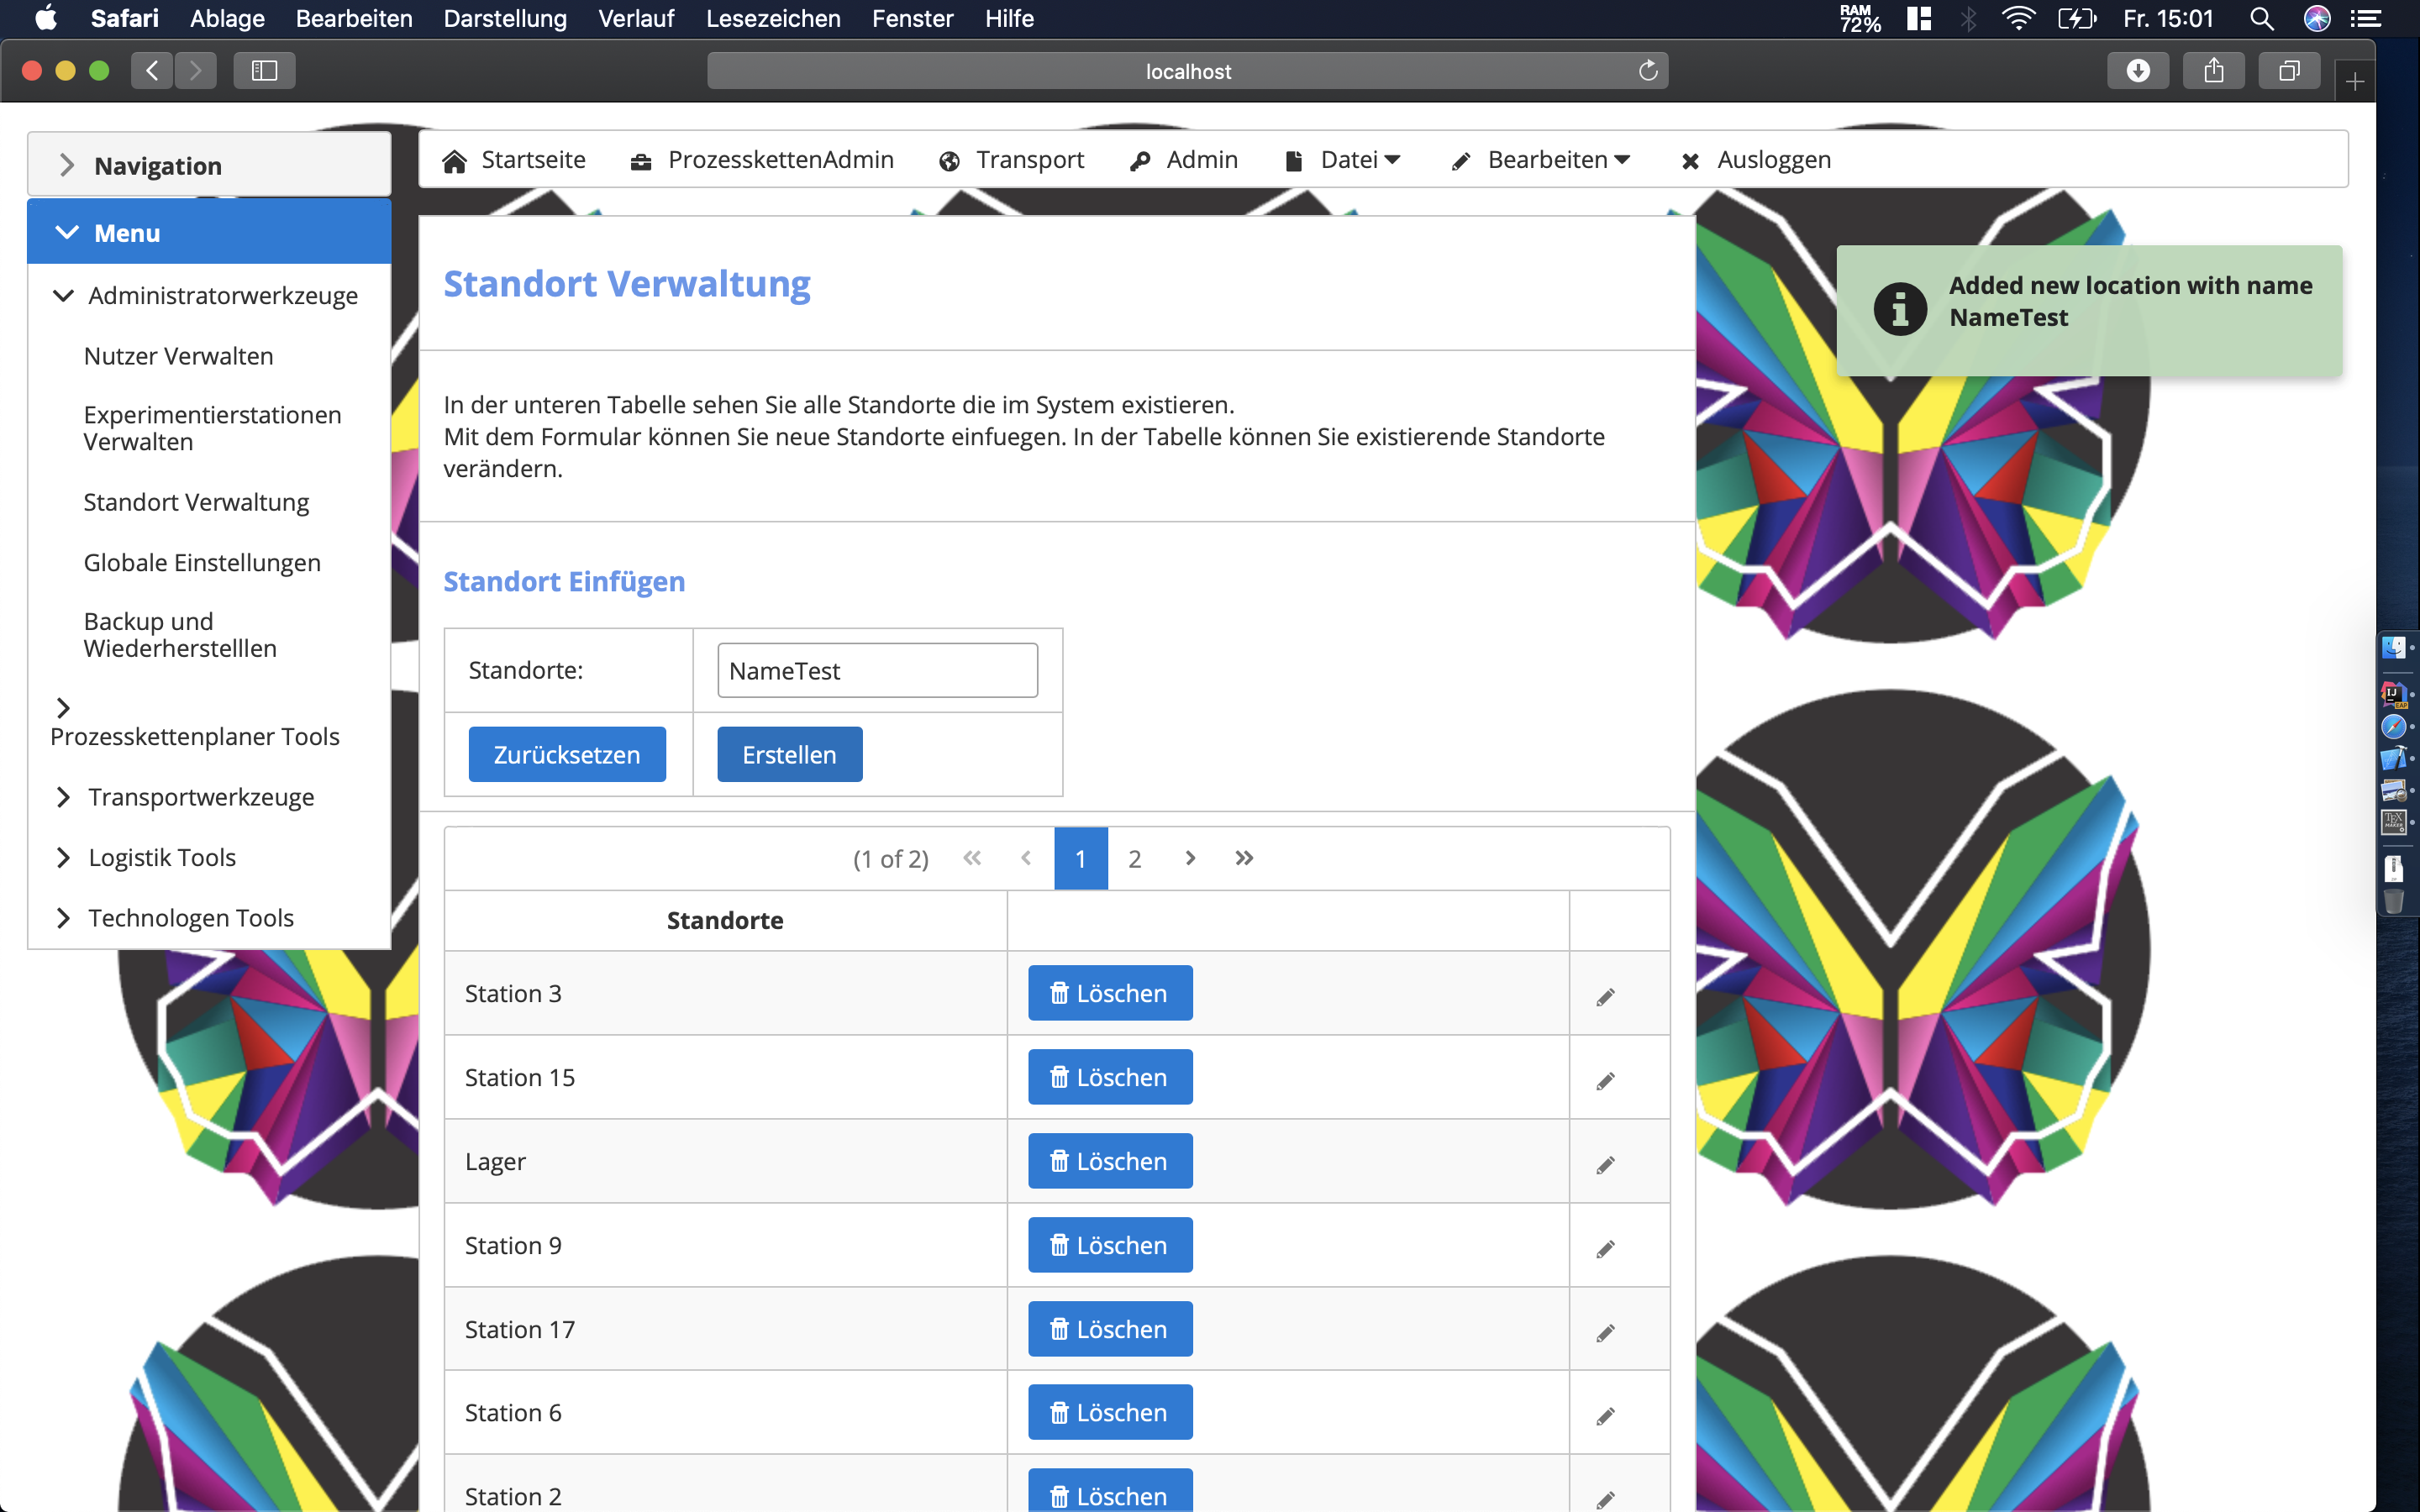
\includegraphics[width=1\textwidth]{Screenshots/4BeschaenigungAddLocation.png}
\textit{Abbildung 3.1.4.2: Standort Erzeugung}
} \\
Die erstellte Station befindet sich in der Tabelle.\\

\hypertarget{sc3.1.4.3}{
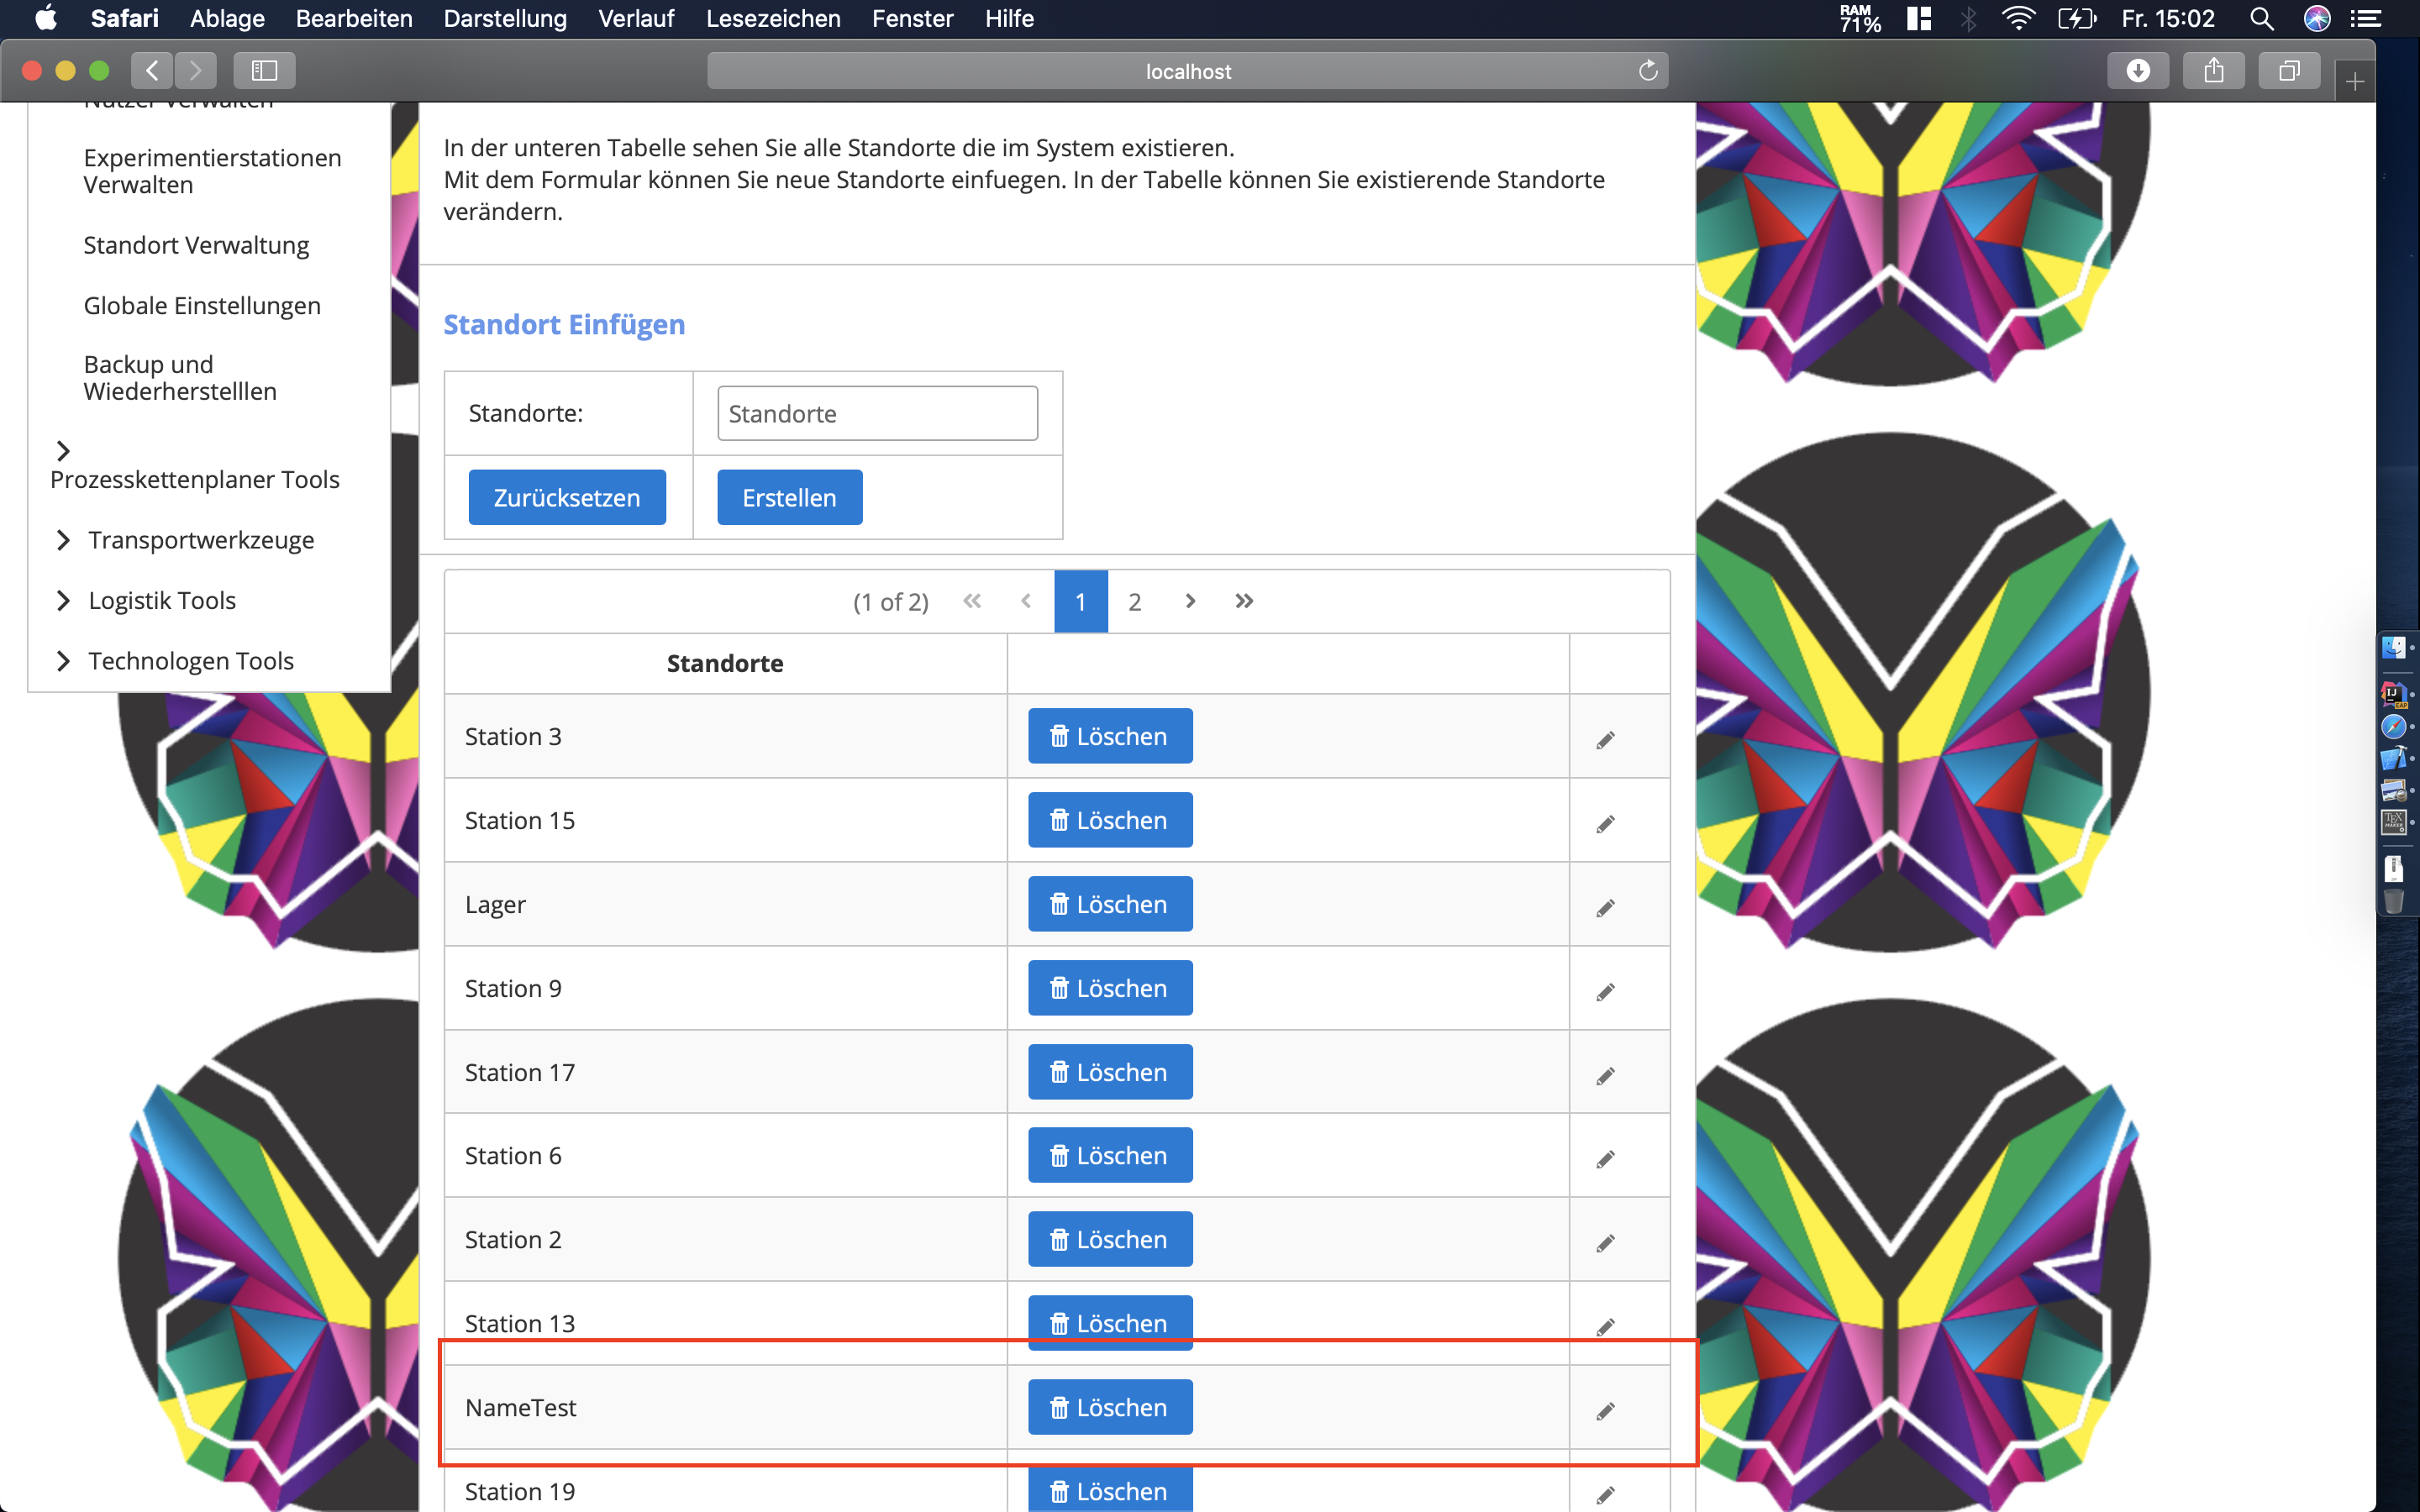
\includegraphics[width=1\textwidth]{Screenshots/4TestExperimentierteEstacion.png}
\textit{Abbildung 3.1.4.3: Standort an der Tabelle}
} \\
Wenn eine Station erstellt wird, wird eine Bestätigungsnachricht durch der Website empfangen.\\

\hypertarget{sc3.1.4.4}{
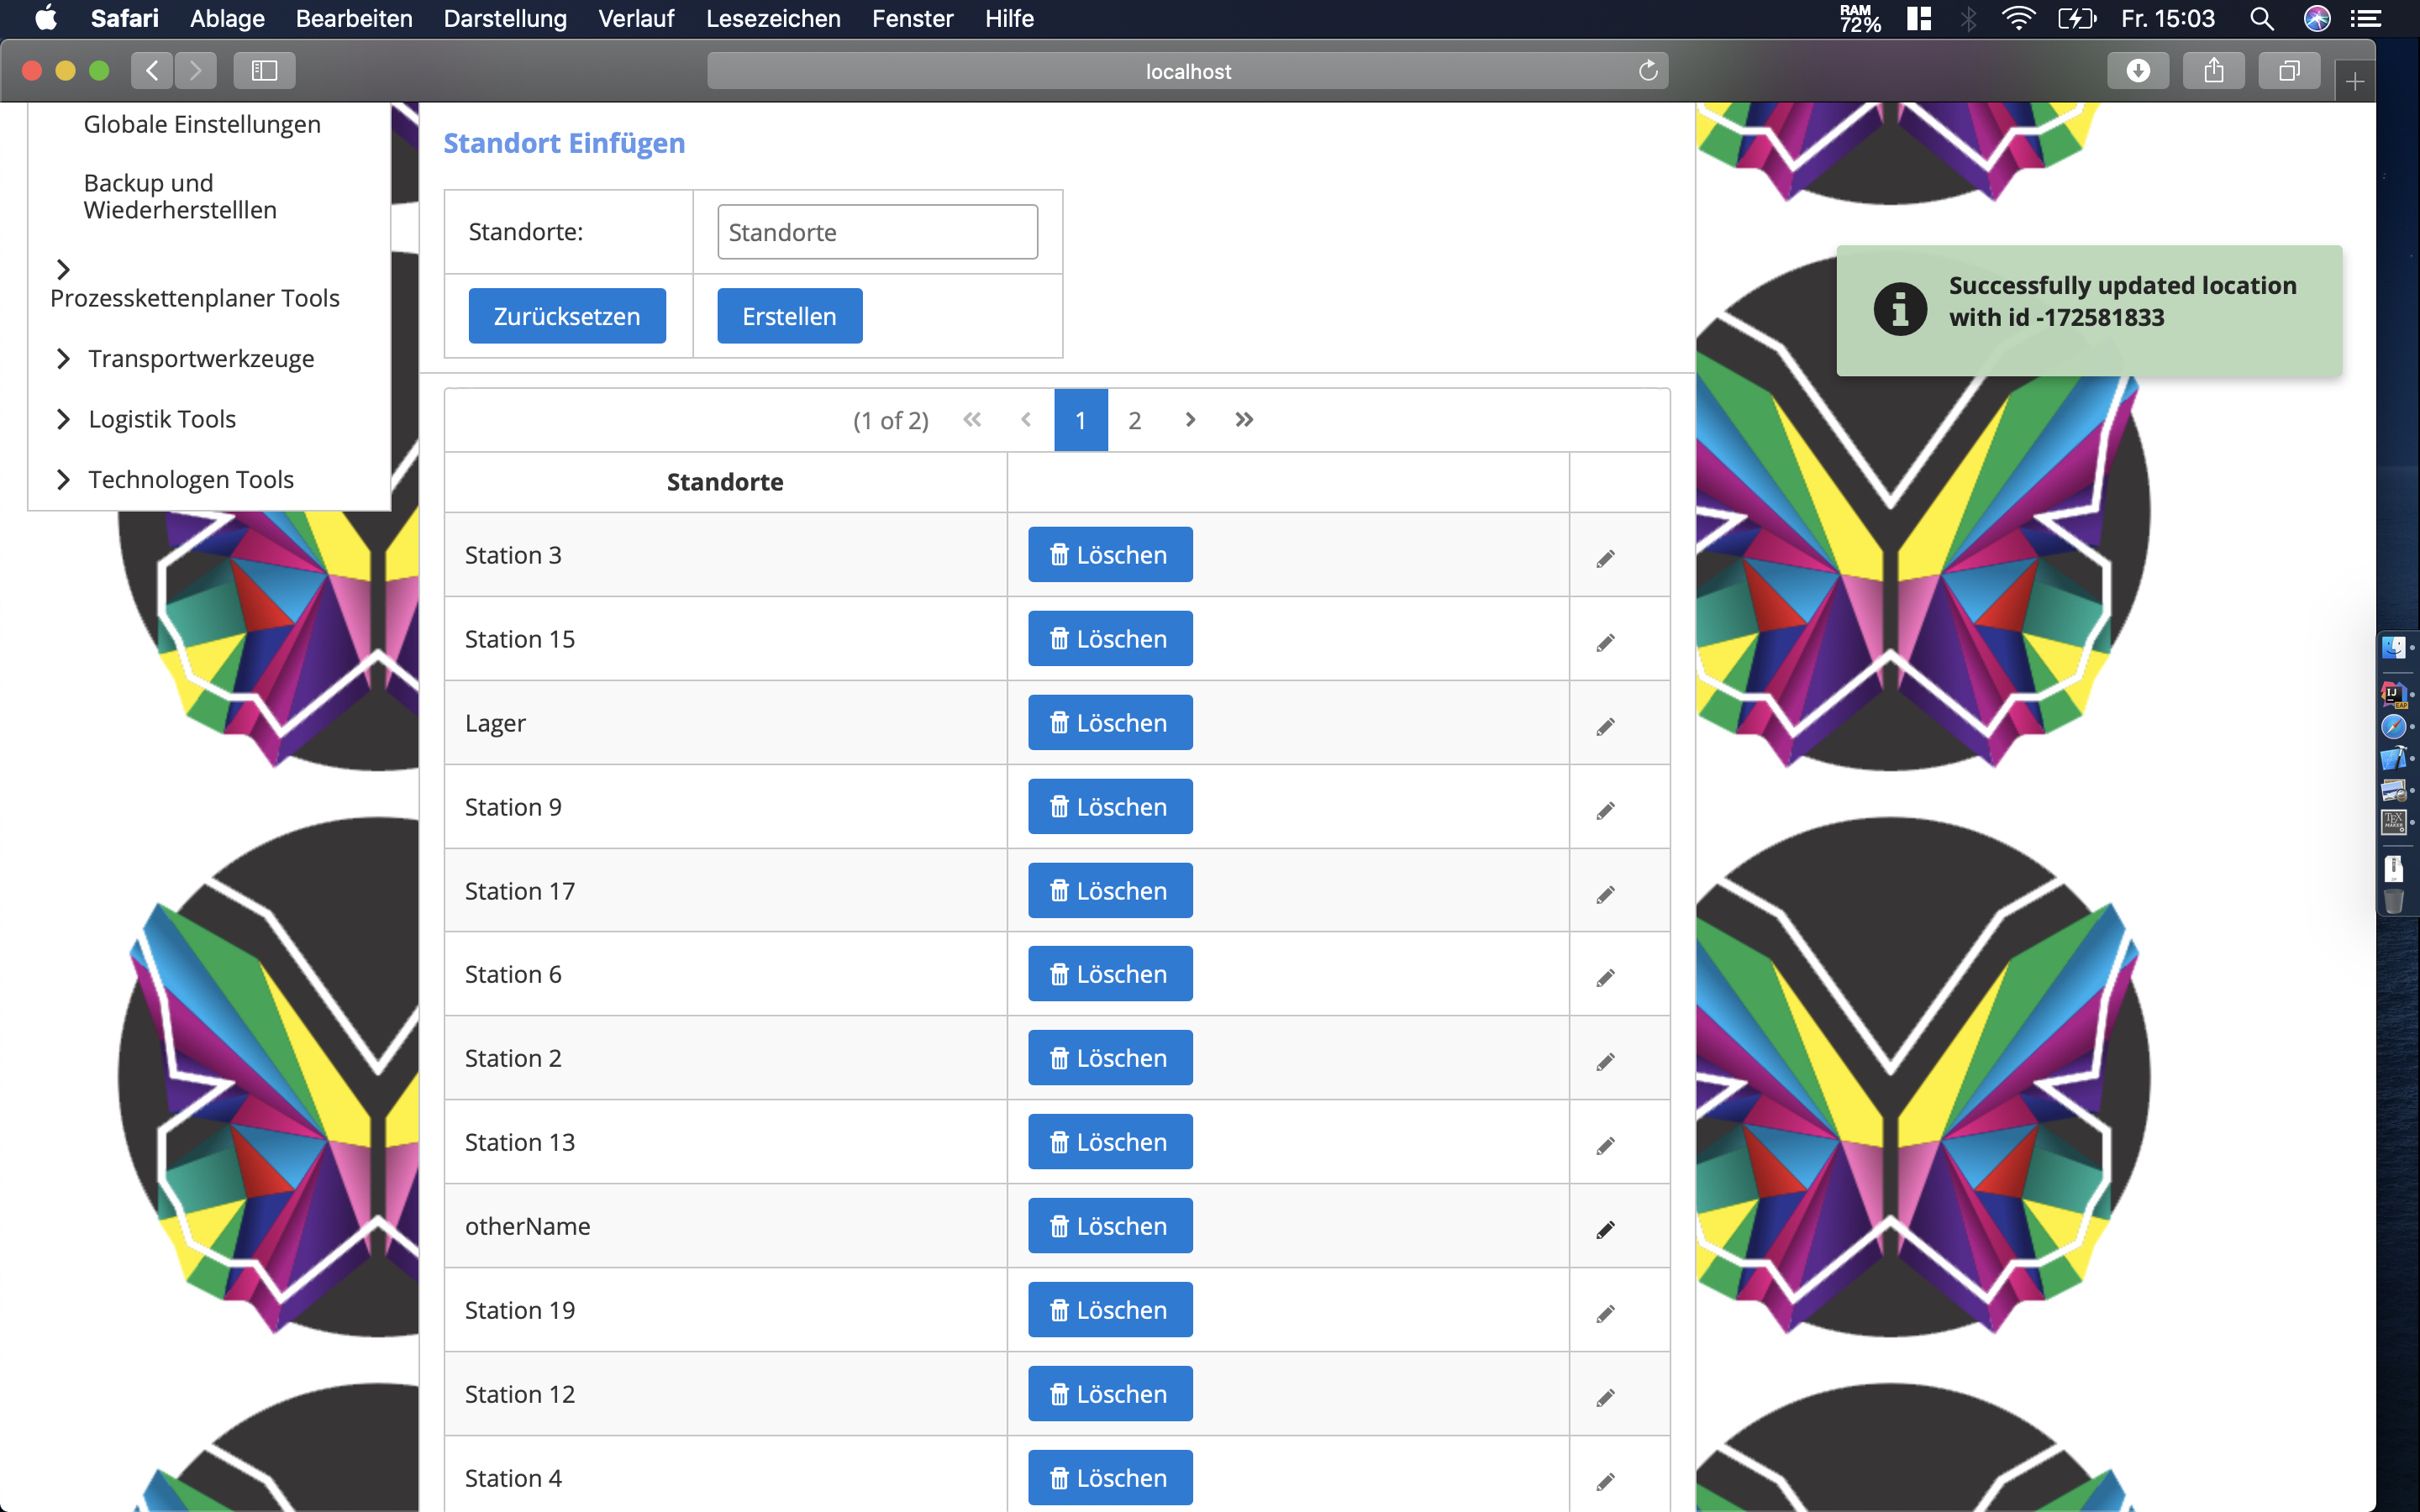
\includegraphics[width=1\textwidth]{Screenshots/4UpdateStantion.png}
\textit{Abbildung 3.1.4.4:  Standort Editieren}
} \\
Auf die gleiche Weise wird beim Drücken der Löschtaste eine Bestätigungsnachricht über die Tabelle der Webseite empfangen.\\

\hypertarget{sc3.1.4.5}{
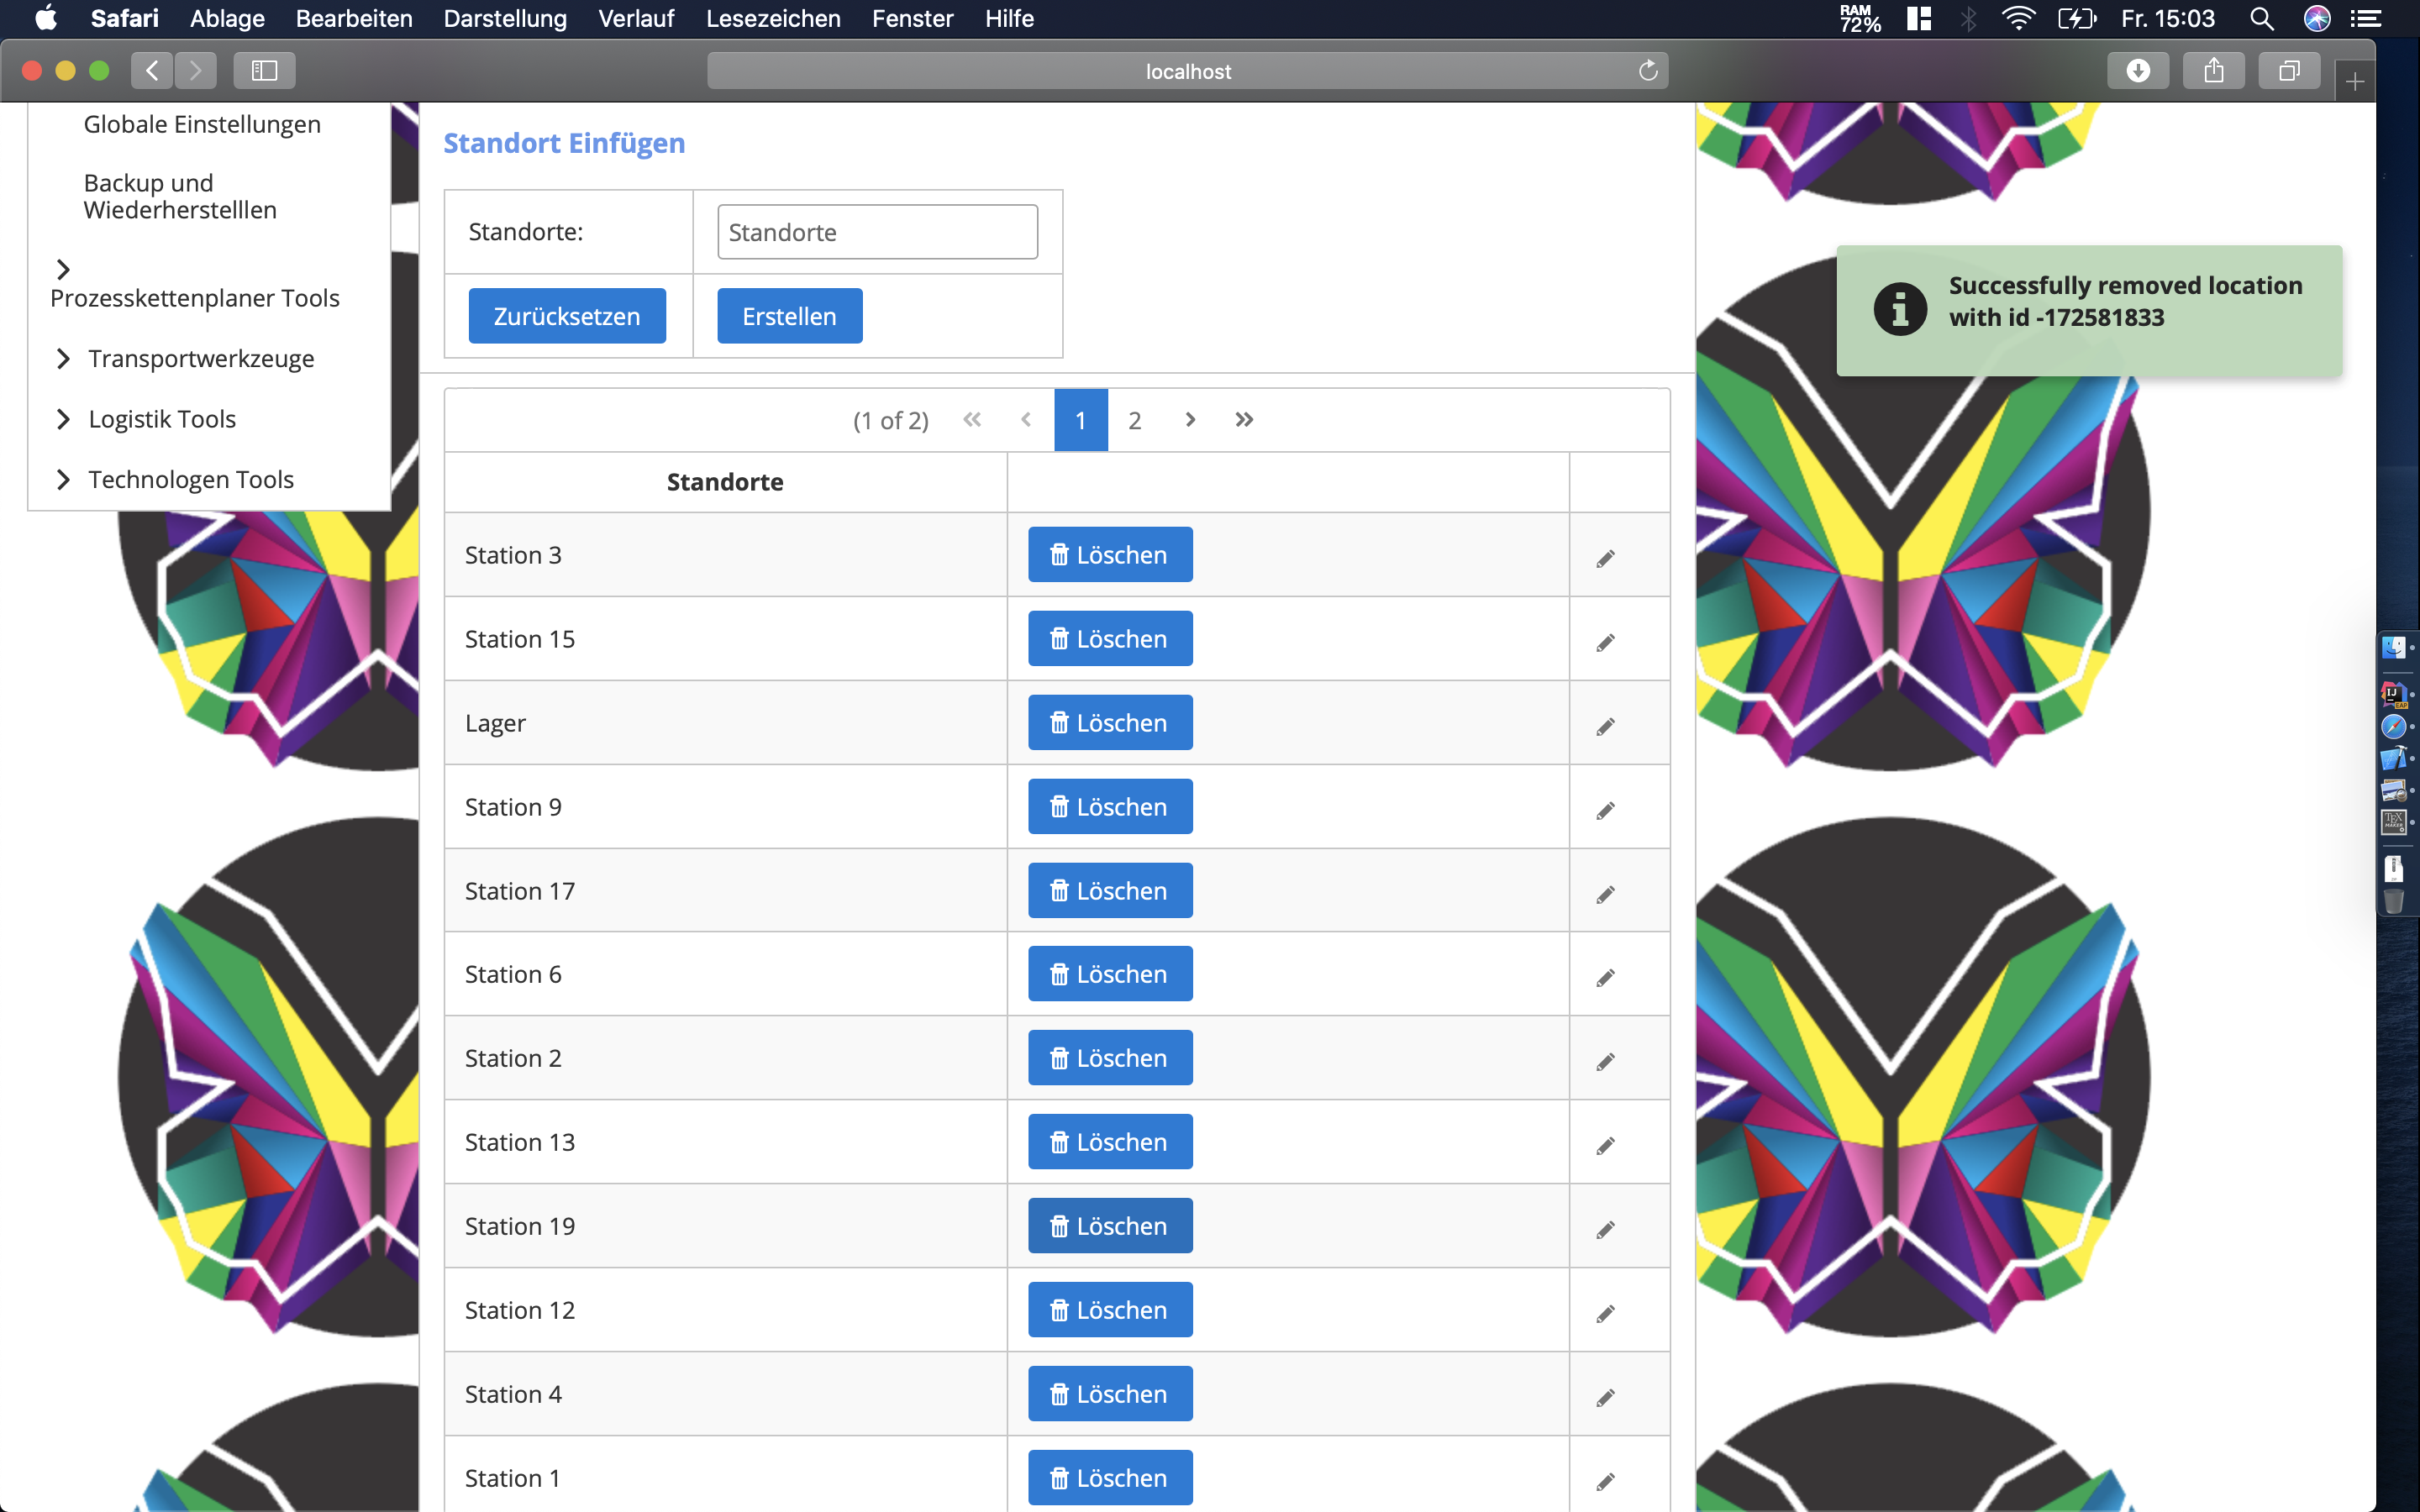
\includegraphics[width=1\textwidth]{Screenshots/4RemoveStation.png}
\textit{Abbildung 3.1.4.5: Standort Entfernen}
} \\
%%

\subsubsection{Anwendungsfall: B Backup}


Um ein Backup der Datenbank zu speichern, muss der Administrator auf der entsprechenden Website auf die knoten Sichern klicken.\\
\hypertarget{sc3.1.5.1}{
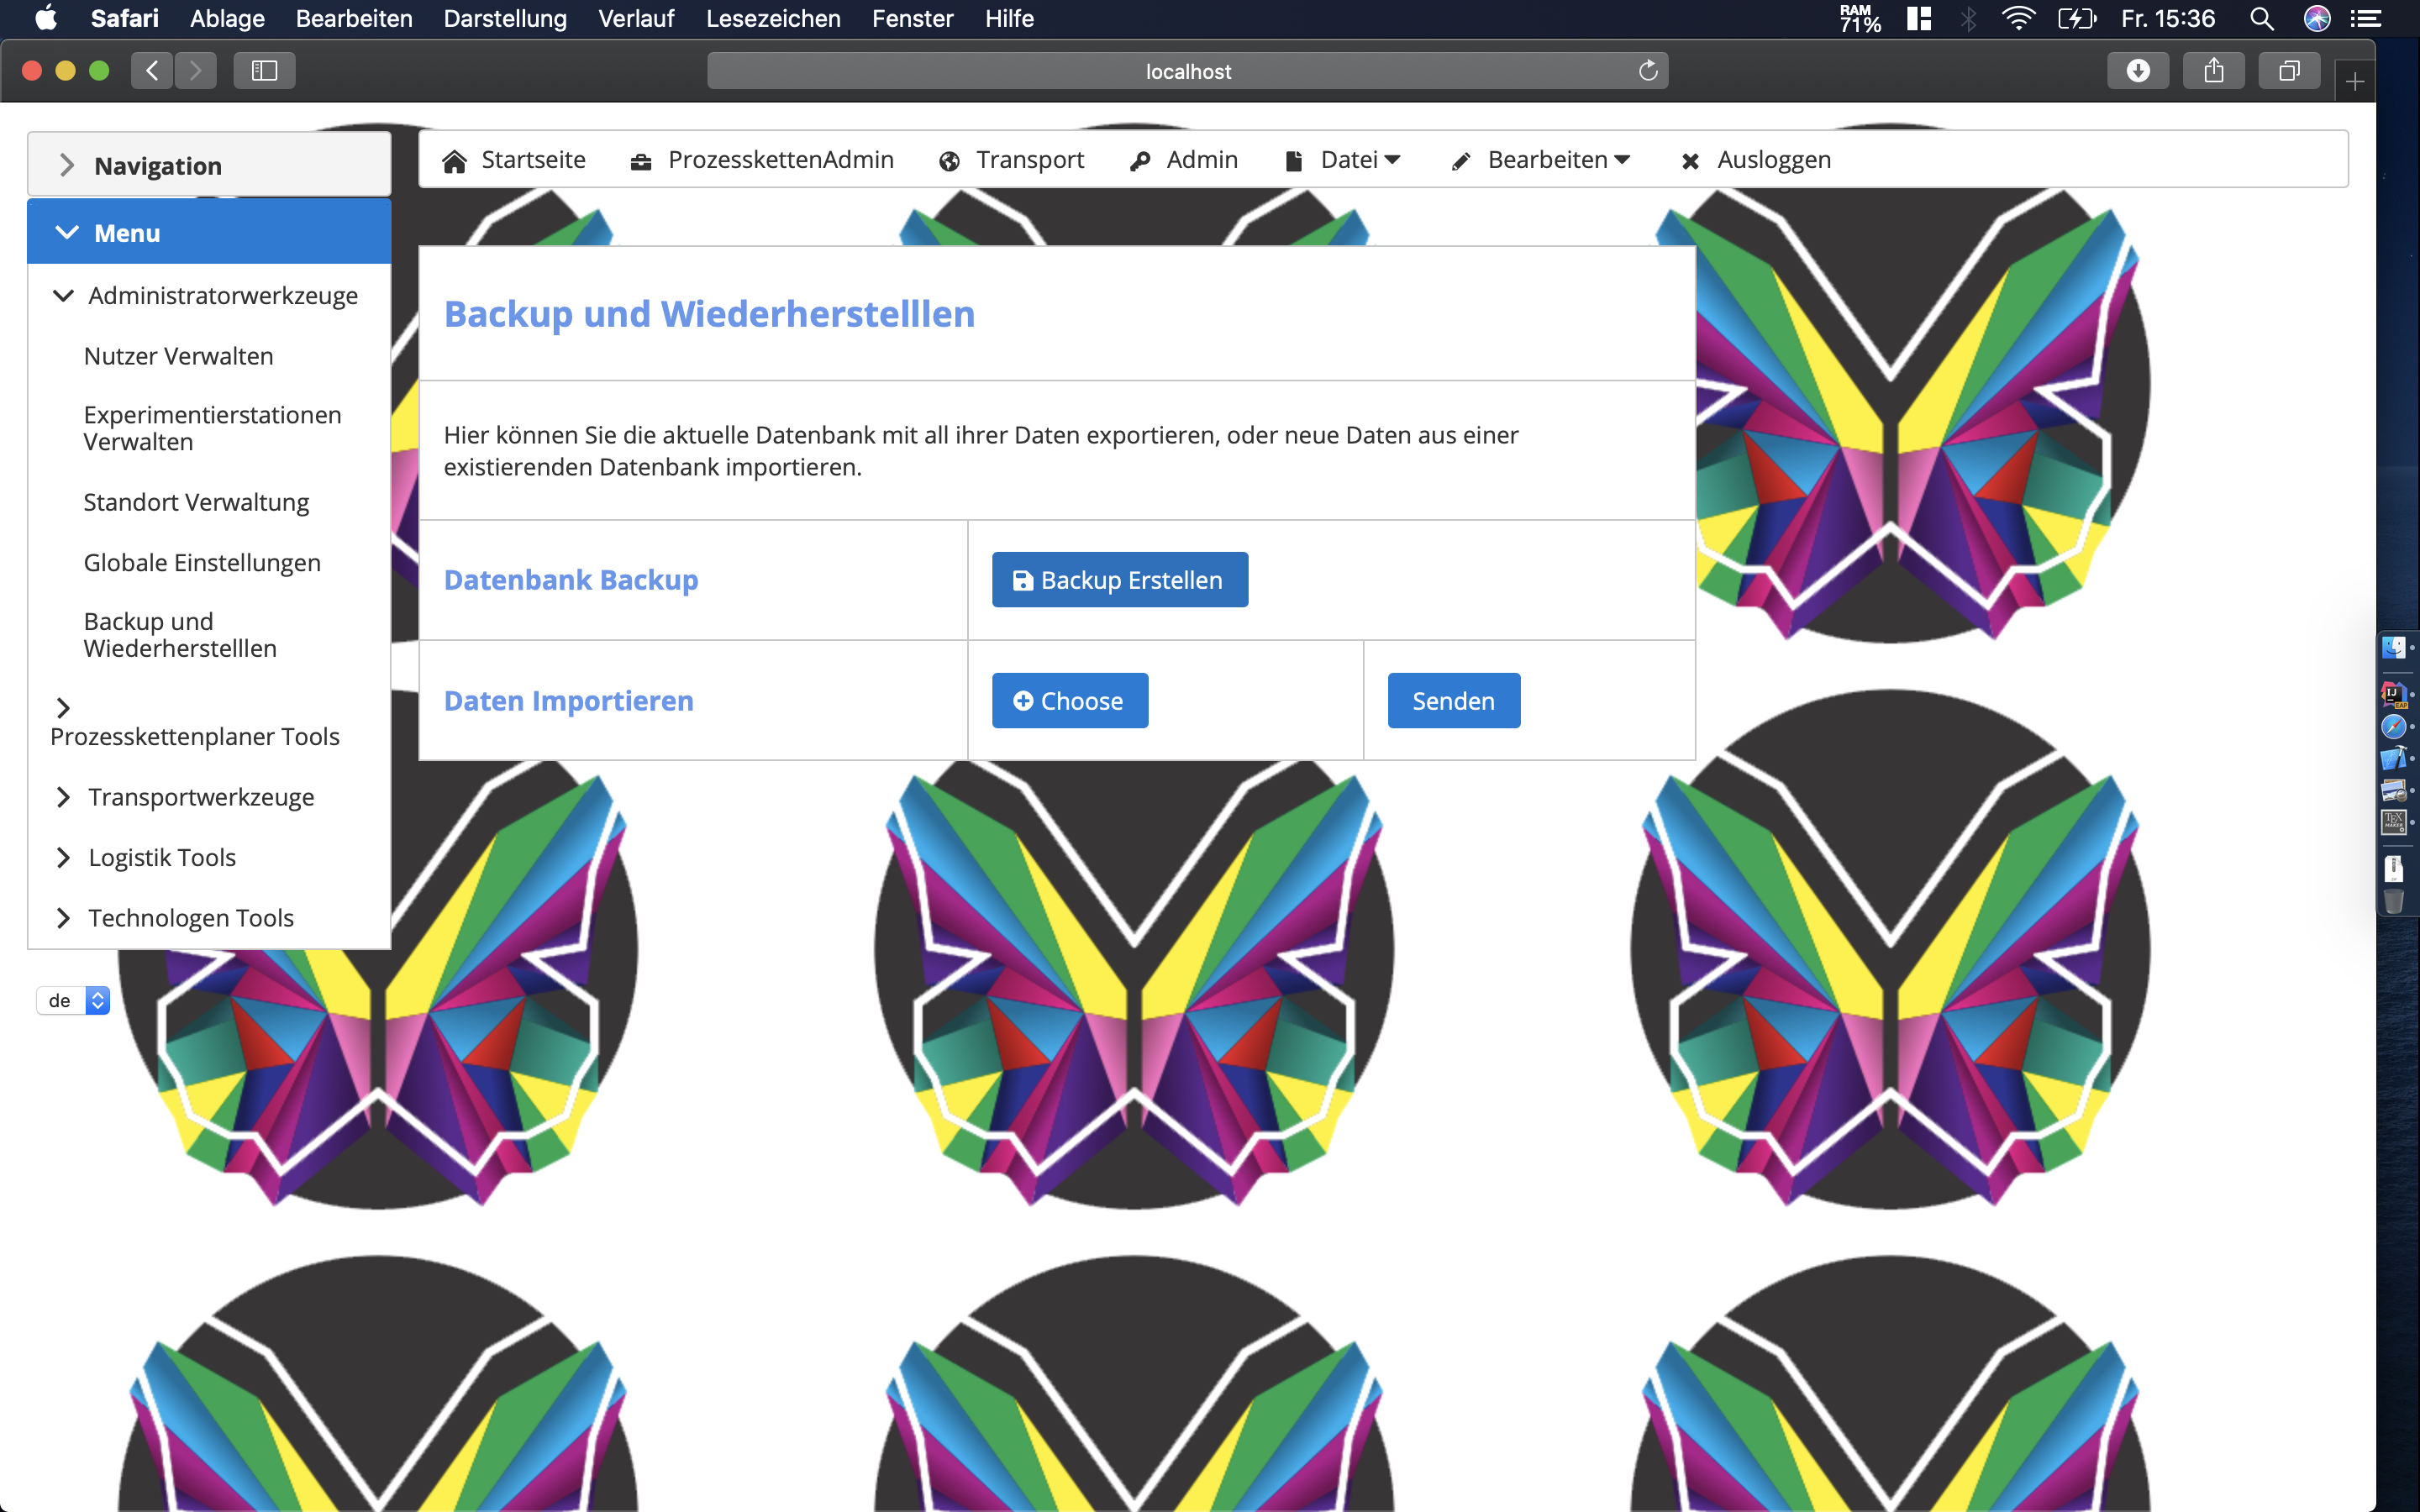
\includegraphics[width=1\textwidth]{Screenshots/5BackFormular.png}
\textit{Abbildung 3.1.5.1: Standort Formular}
} \\

Wenn das Backup generiert wird, sendet die Webseite eine Bestätigungsnachricht.\\
\hypertarget{sc3.1.5.2}{
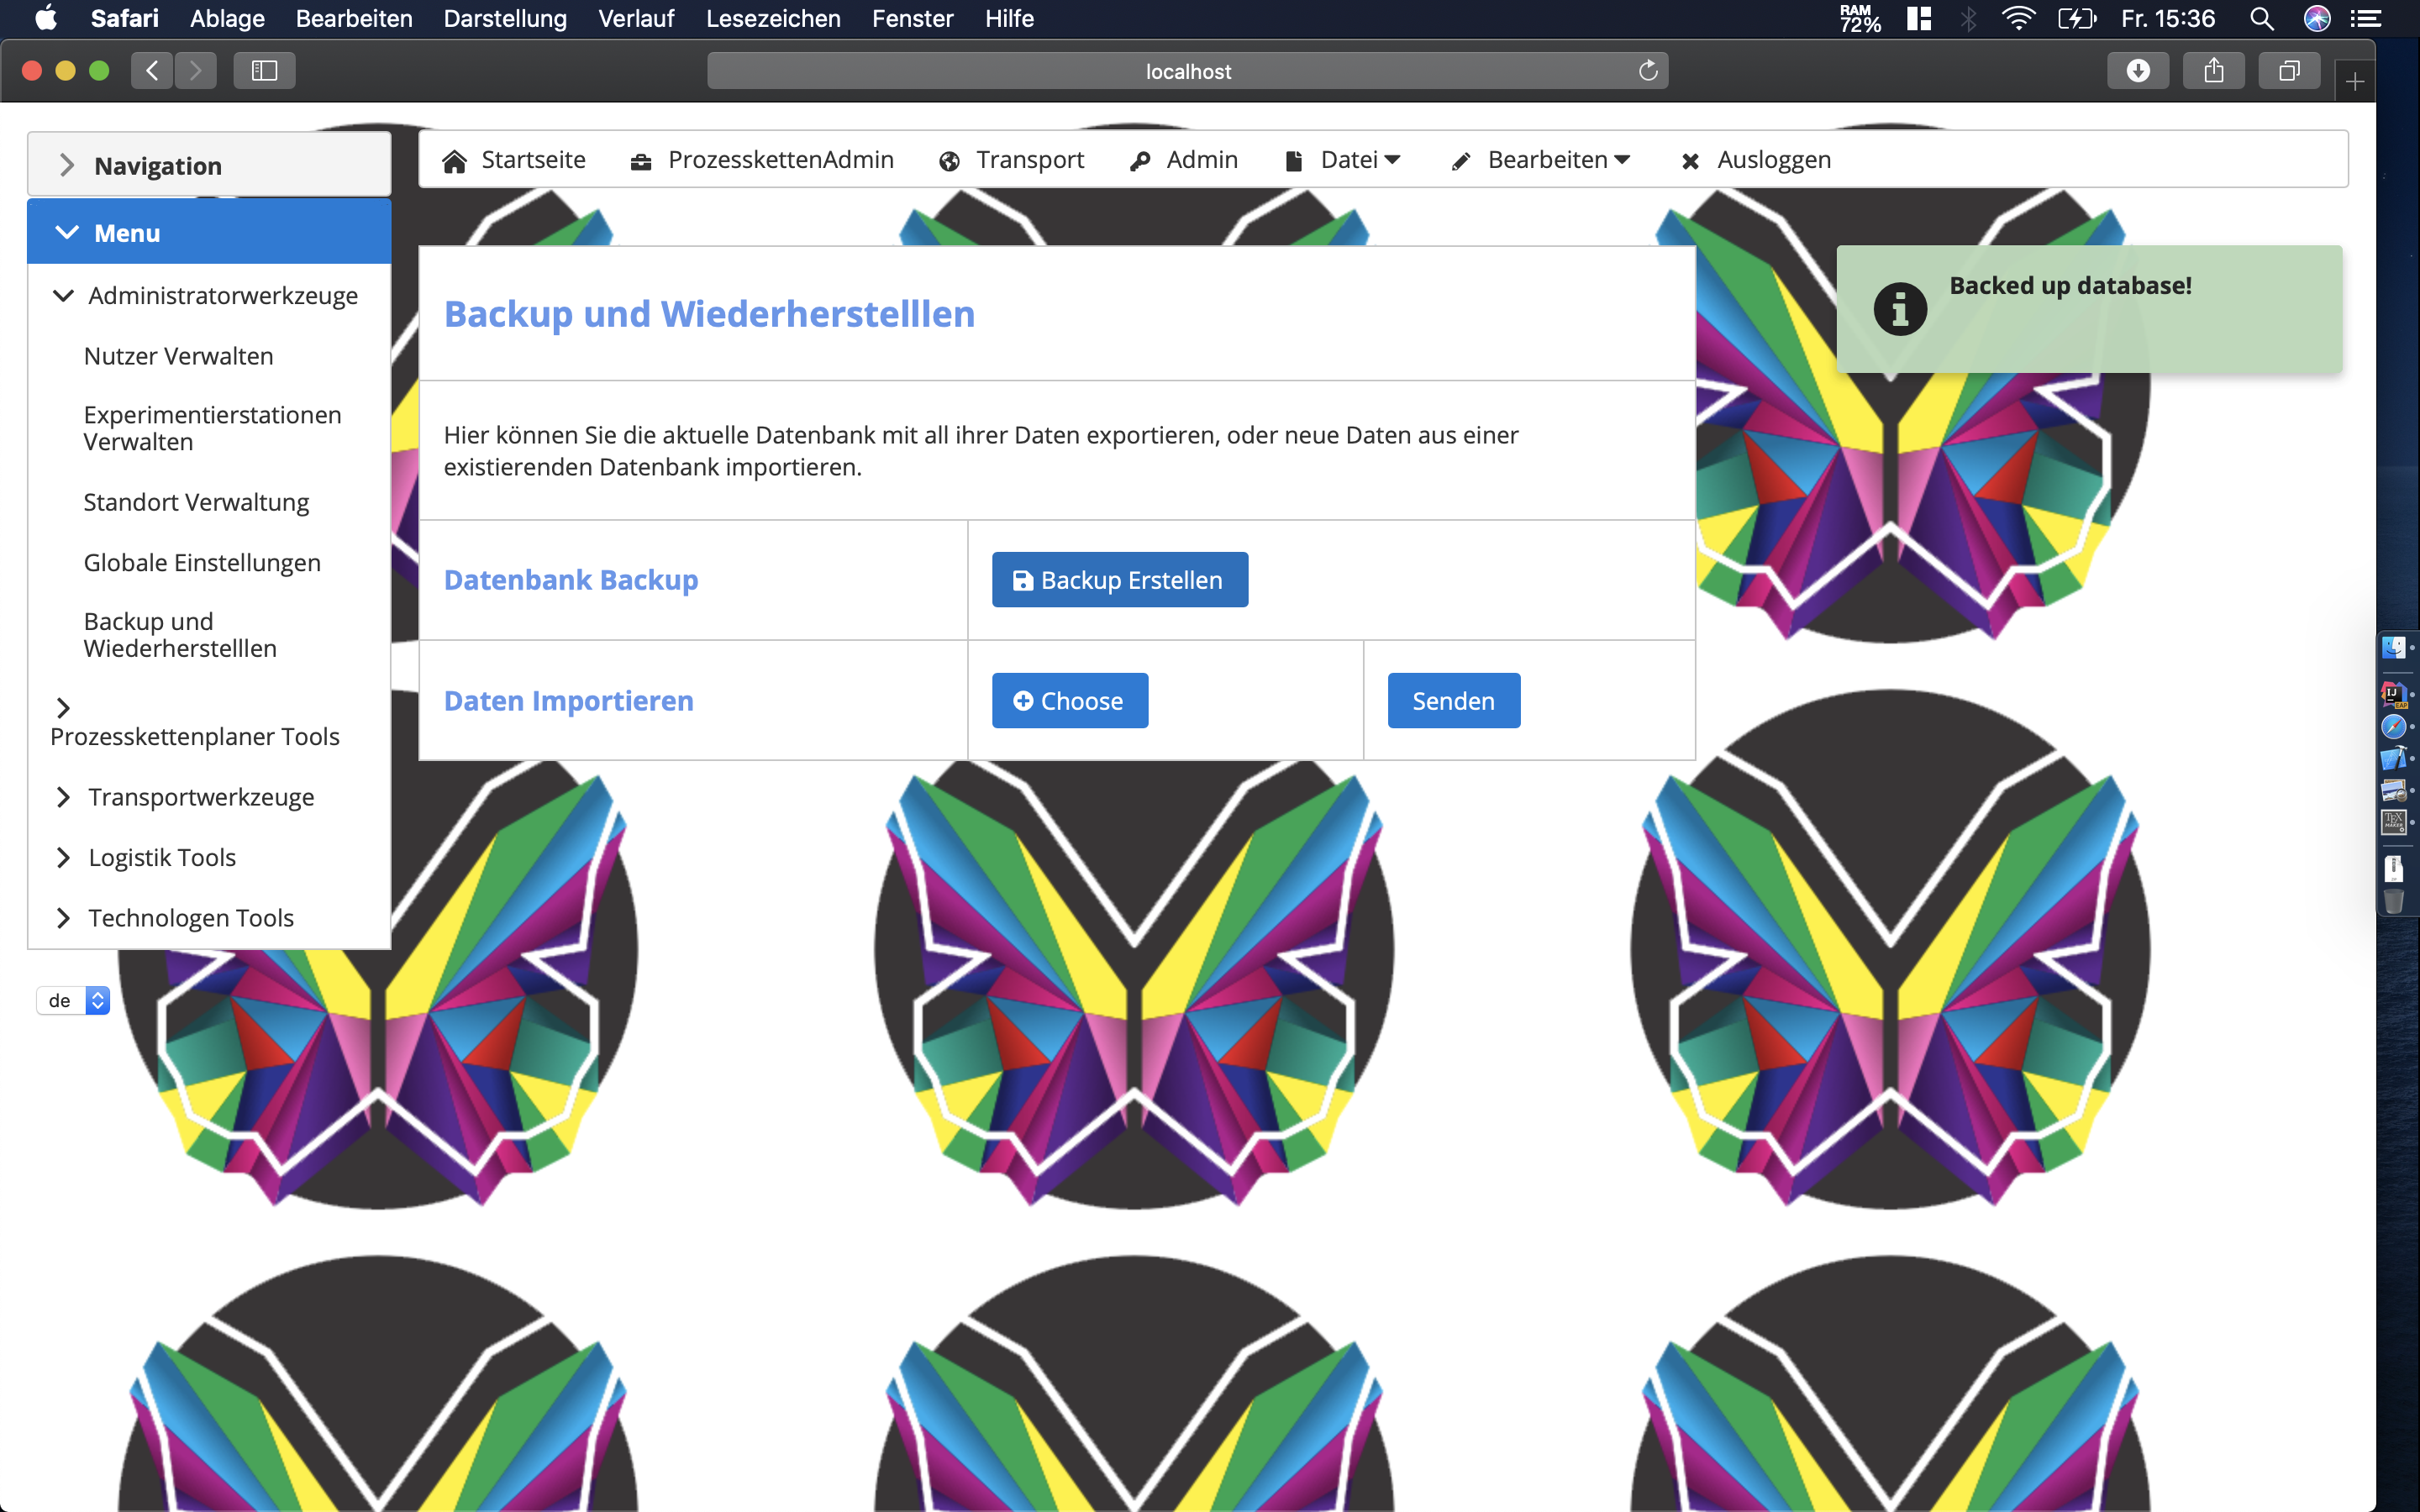
\includegraphics[width=1\textwidth]{Screenshots/5BackGenerated.png}
\textit{Abbildung 3.1.5.2: Standort Formular}
} \\

Die Generierung der Datei wurde getestet.\\

\hypertarget{sc3.1.5.3}{
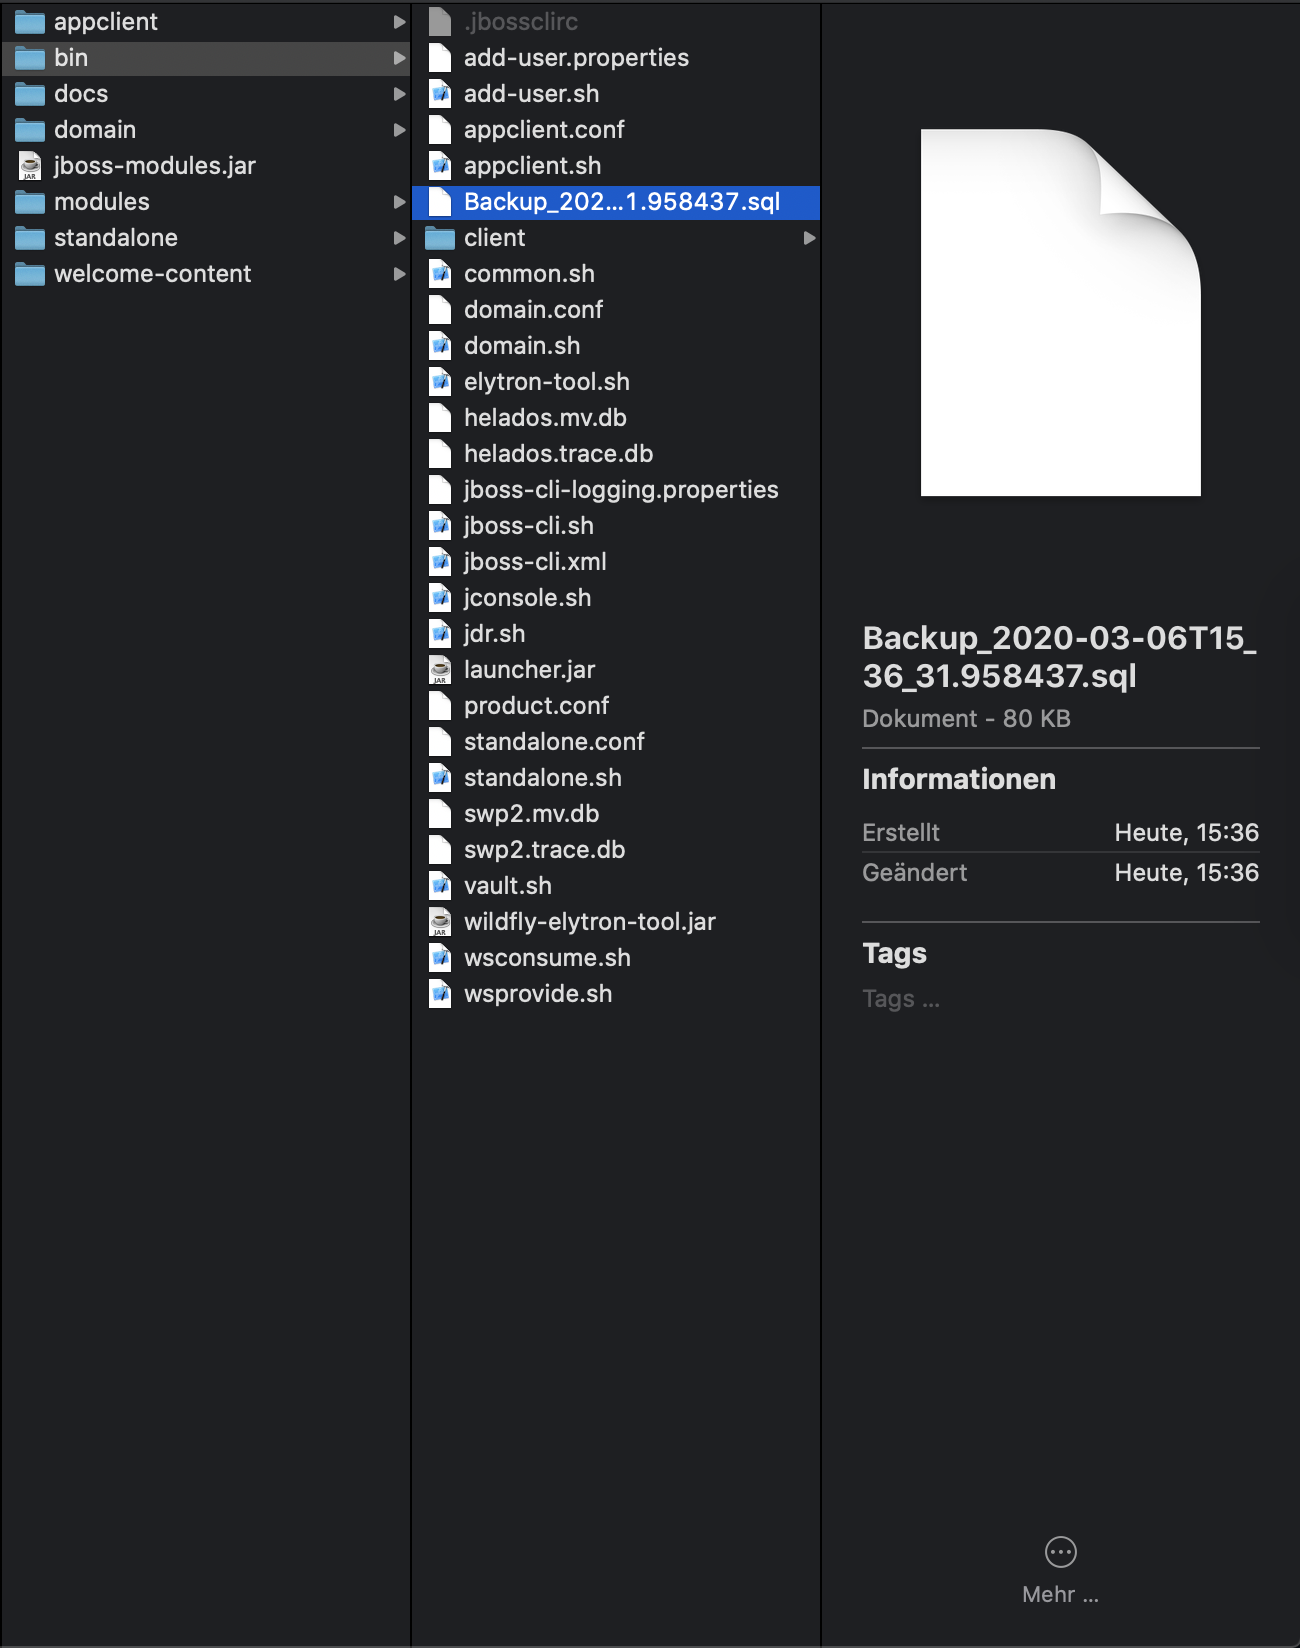
\includegraphics[width=1\textwidth]{Screenshots/5BackUpDatei.png}
\textit{Abbildung 3.1.5.3: Standort Formular}
} \\
Um den Import der Datenbanken zu testen, wurden alle Systembenutzer entfernt. Sobald eine Datendatei mit neuen Benutzern importiert wurde.\\
\hypertarget{sc3.1.5.4}{
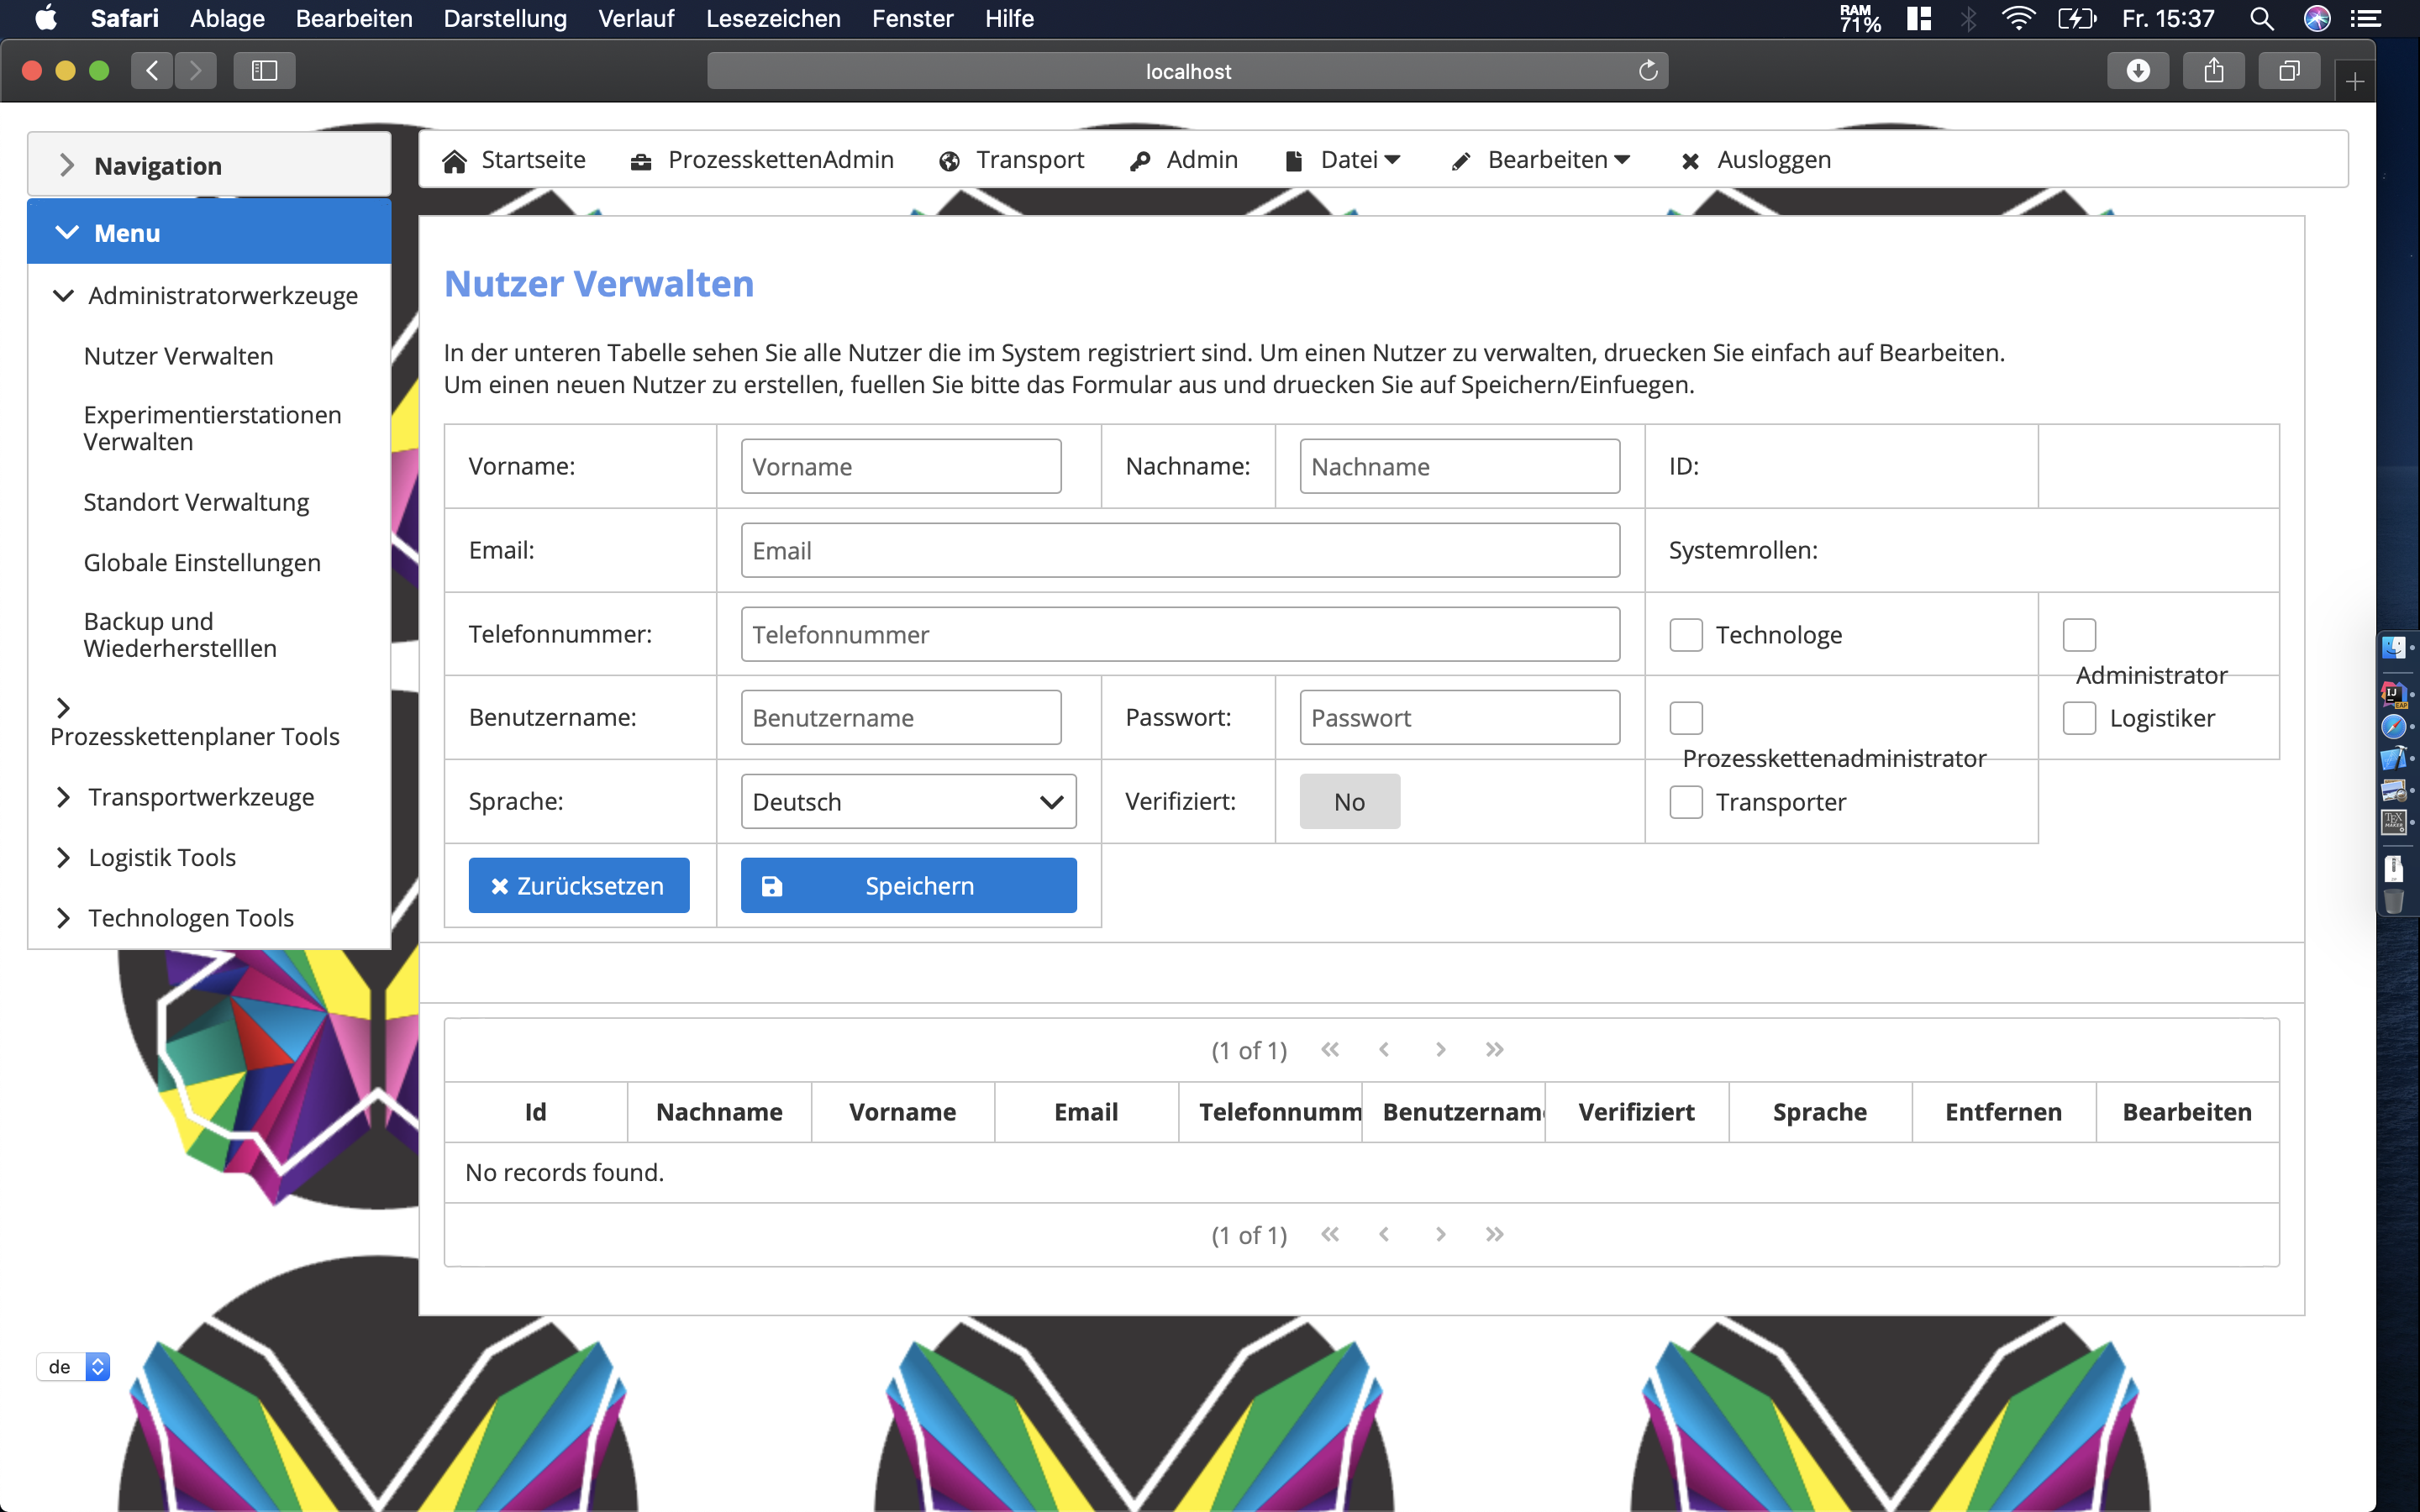
\includegraphics[width=1\textwidth]{Screenshots/5NotUsers.png}
\textit{Abbildung 3.1.5.4: Standort Formular}
} \\

\hypertarget{sc3.1.5.5}{
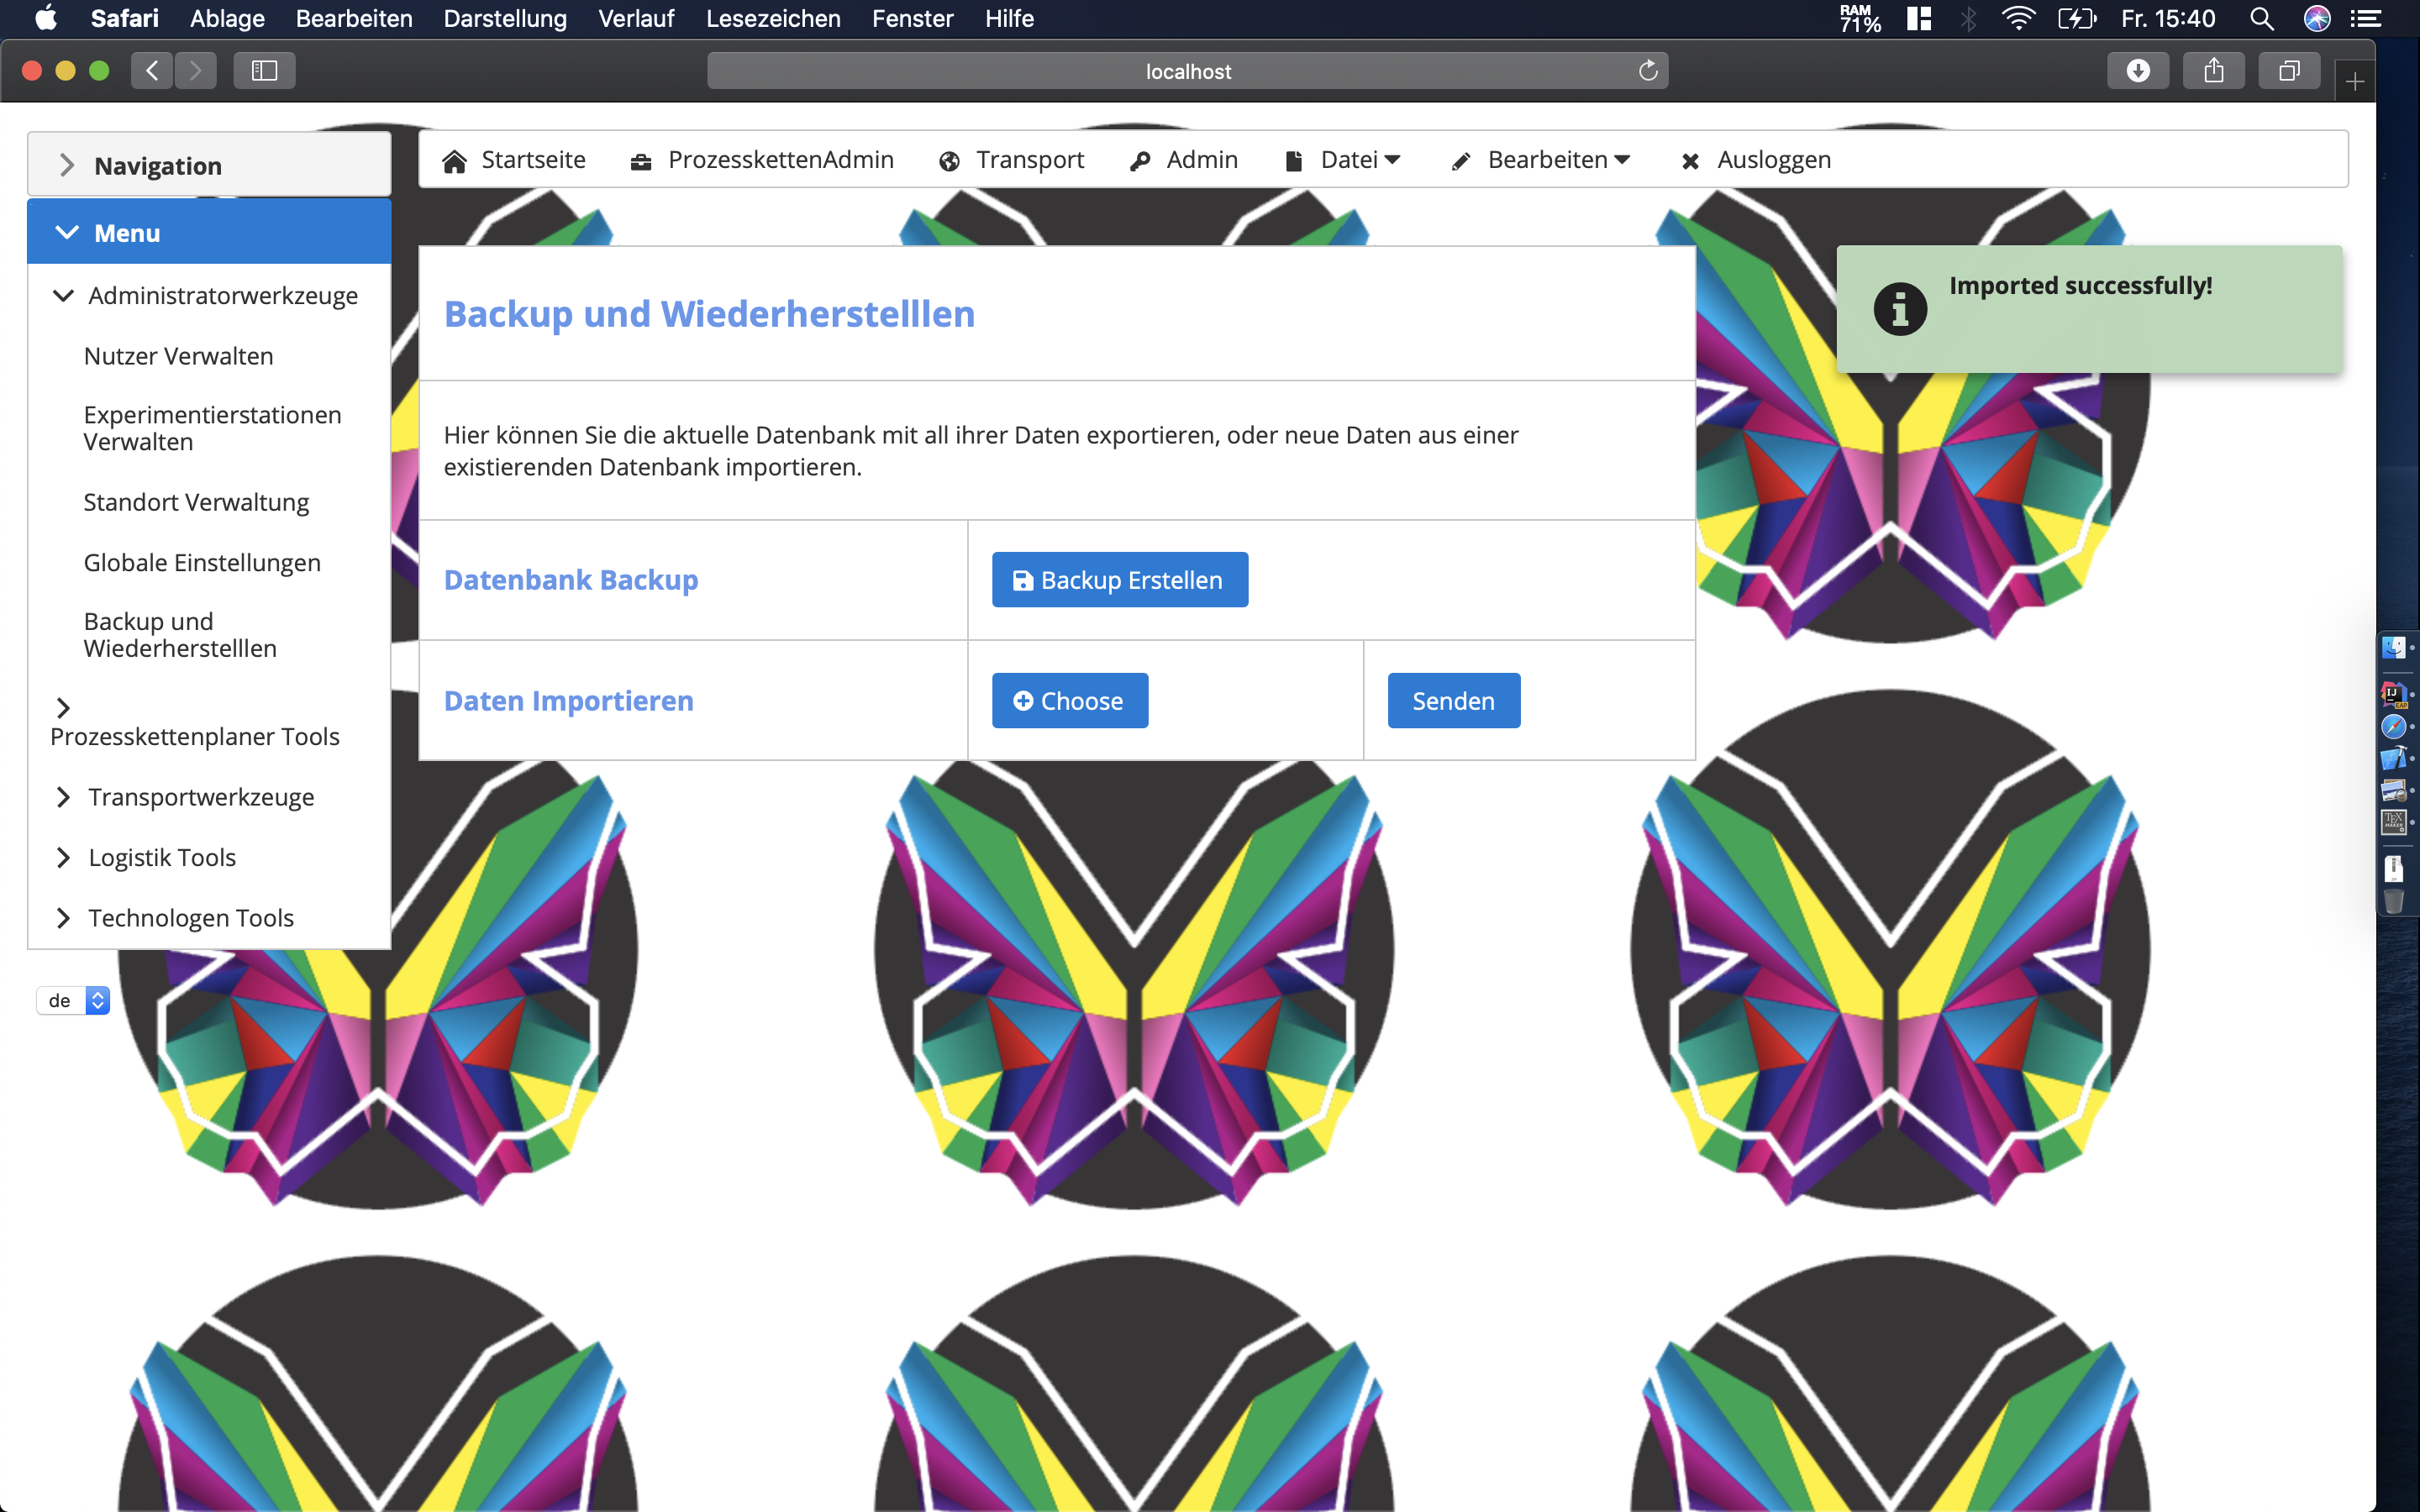
\includegraphics[width=1\textwidth]{Screenshots/5BackImported.png}
\textit{Abbildung 3.1.5.5: Standort Formular}
} \\
In der folgenden Grafik sehen Sie, dass die Benutzer erfolgreich aktualisiert wurden.\\

\hypertarget{sc3.1.5.6}{
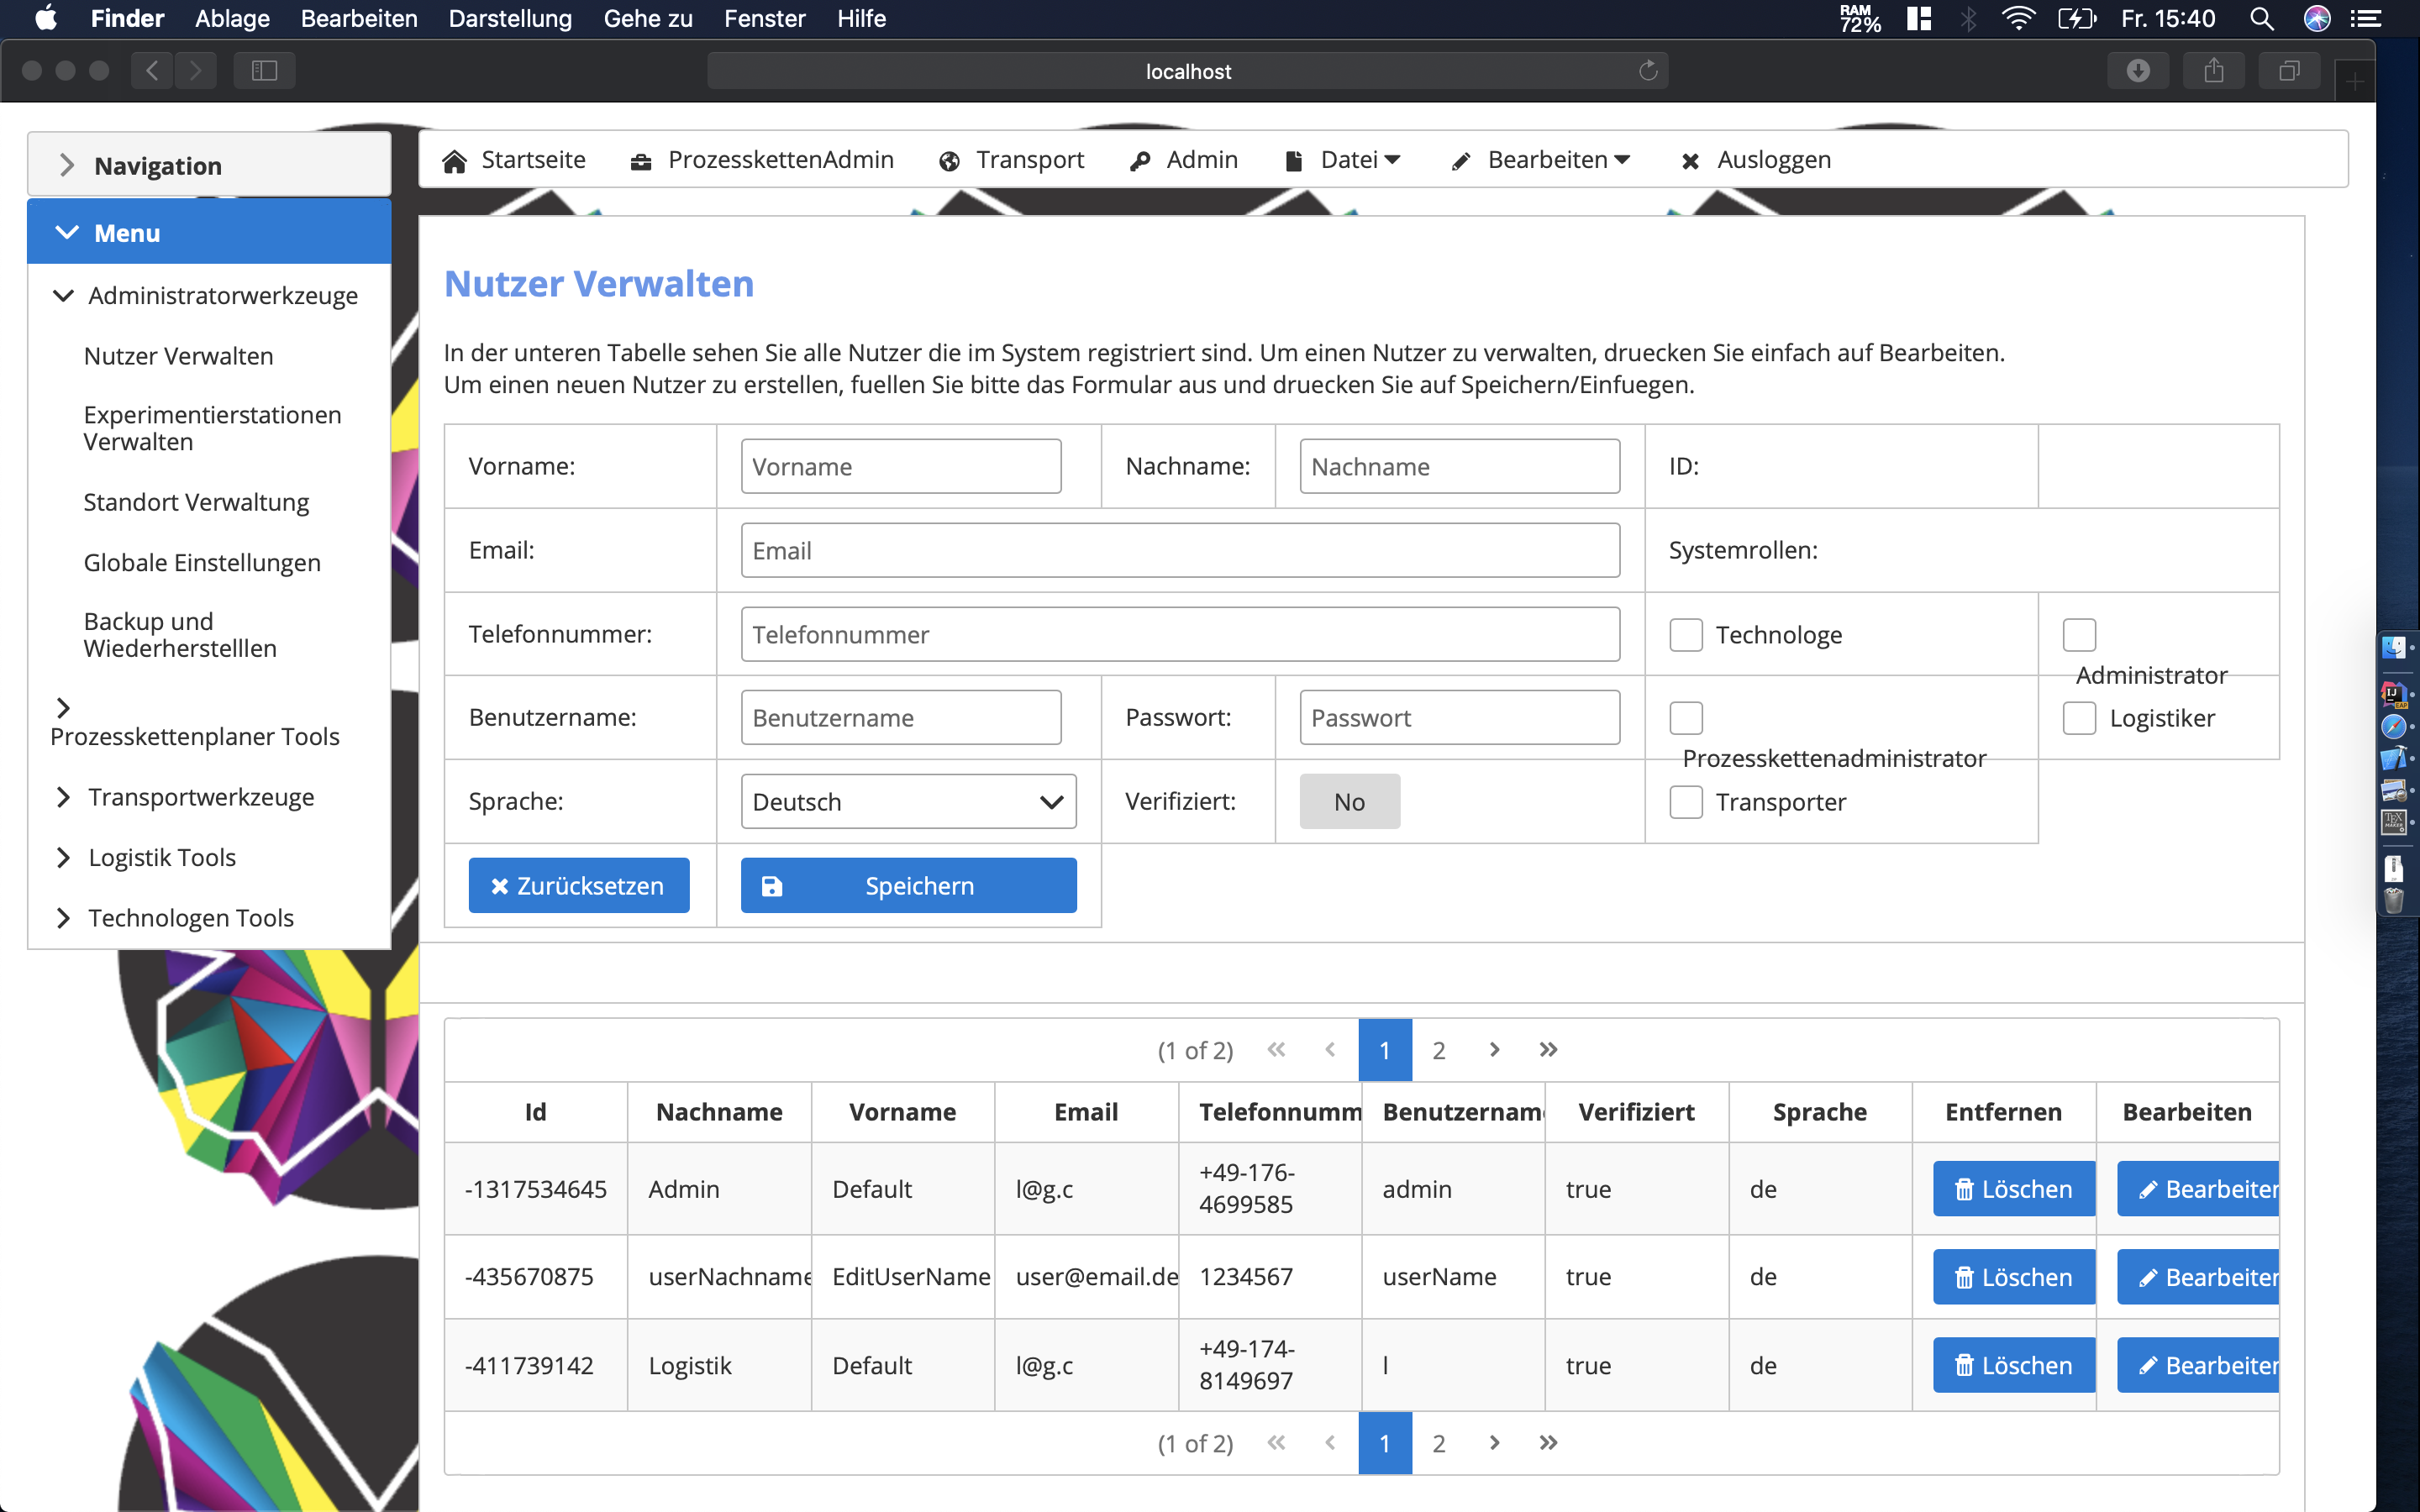
\includegraphics[width=1\textwidth]{Screenshots/5AddUsers.png}
\textit{Abbildung 3.1.5.6: Standort Formular}
} \\

%%

\subsubsection{Anwendungsfall: pk 1}

%%

\subsubsection{Anwendungsfall: pk 2}

%%

\subsubsection{Anwendungsfall: pk 3}

%%

\subsubsection{Anwendungsfall: pk 4}

%%

\subsubsection{Anwendungsfall: pk 5}

%%

\subsubsection{Anwendungsfall: pk 6}

%%

\subsubsection{Anwendungsfall: pk 7}

%%

\subsubsection{Anwendungsfall: pk8 }

%%

\subsubsection{Anwendungsfall: pk9}

%%

\subsubsection{Anwendungsfall: tr 1}

%%

\subsubsection{Anwendungsfall: tr 2}

%%

\subsubsection{Anwendungsfall: log 1}

%%

\subsubsection{Anwendungsfall: log 2}

%%

\subsubsection{Anwendungsfall: log 3}

%%

\subsubsection{Anwendungsfall: log 4}

%%

\subsubsection{Anwendungsfall: log 5}

%%

\subsubsection{Anwendungsfall: log 6}

%%

\subsubsection{Anwendungsfall: log 7}

%%

\subsubsection{Anwendungsfall: Beispiel 5}

%%

\subsubsection{Anwendungsfall: Beispiel 5}

%%%%%%%%%%%%

\subsection{Automatisierte Funktionstests}

\subsubsection{Anwendungsfall: Beispiel 1}

%%

\subsubsection{Anwendungsfall: Beispiel 2}

%%

\subsubsection{Anwendungsfall: Beispiel 3}

%%

\subsubsection{Anwendungsfall: Beispiel 4}

%%

\subsubsection{Anwendungsfall: Beispiel 5}

%%%%%%%%%%%%%%%%%%%%%%%%%%%%%%%%%%%%%%%%%%%%%%%%%%%%%%%%%%%%%%%%%%%%%%%%

\end{document}














